%!
%! Copyright (C) 2015 - Present Andrea Dal Corso 
%! This file is distributed under the terms of the
%! GNU General Public License. See the file `License'
%! in the root directory of the present distribution,
%! or http://www.gnu.org/copyleft/gpl.txt .
%!
\documentclass[12pt,a4paper]{article}
\def\version{0.6.0}
\def\qe{{\sc Quantum ESPRESSO}}
\def\tpw{{\sc THERMO\_PW}}

\usepackage{html}
\usepackage{color}

\definecolor{web-blue}{rgb}{0,0.5,1.0}
\definecolor{coral}{rgb}{1.0,0.5,0.3}
\definecolor{red}{rgb}{1.0,0,0.0}
\definecolor{green}{rgb}{0.,1.0,0.0}

\usepackage{graphicx}

\textwidth = 17cm
\textheight = 24cm
\topmargin =-1 cm
\oddsidemargin = 0 cm

\def\pwx{\texttt{pw.x}}
\def\phx{\texttt{ph.x}}
\def\configure{\texttt{configure}}
\def\PWscf{\texttt{PWscf}}
\def\PHonon{\texttt{PHonon}}
\def\thermo{\texttt{thermo\_pw}}
\def\make{\texttt{make}}

\begin{document} 
\author{Andrea Dal Corso (SISSA - Trieste)}
\date{}

%\def\SissaImage{./sissa_on_white.png}

\title{
%  \includegraphics[width=6cm]{\SissaImage}\\
  \vskip 1cm
  {\color{red}\Huge Point groups in \qe\ and \tpw\ }
  \Large (version \version)
}

\maketitle

\tableofcontents

\newpage
\section{\color{coral}Introduction}
\qe\ and \tpw\ can determine the point group of a
solid, the symmetry of its physical properties, the symmetry
of the electronic wavefunctions and of the phonon modes. The proper interpretation
of these symmetry information requires the knowledge of the conventions on the 
underlying point groups. This small guide illustrates these conventions
for a better interpretation of the output of these codes. \\
For each point group we give: 
\begin{itemize}

\item
The crystal system and the Bravais lattices compatible with the point
group.

\item
The Laue class.

\item
A brief description of the symmetry operations. 
A description of the possible orientations of the rotation axes and of the 
mirror planes with respect to the Cartesian axes.

\item
The character table and a description of the main characteristic of each 
irreducible representation.

\item
The character table of the double group and a description of the main 
characteristic of each irreducible representation.

\item
The character tables of the inequivalent projective representations for the 
groups that have them.

\item
A list of the possible subgroups and the relative orientation of the symmetry
elements of these subgroups.

\item
A subgroup compatibility table of the irreducible representations.

\item
A subgroup compatibility table of the double-group irreducible representations. 

\end{itemize}
Other information on the crystallographic points groups used by the code 
not reported in the present manual can be obtained using the tool 
\texttt{crystal\_point\_group.x}. Among them we mention:
\begin{itemize}

\item A complete listing of the symmetry operations of each group
and their $O(3)$ and $SU(2)$ matrices.

\item A complete listing of all point subgroups and supergroups.

\item A multiplication table of all the double point groups.

\item A compatibility table of all the projective representations.

\item A table of all the Kronecker products of the representations and
their decomposition into the irreducible or projective representations
of all the subgroups.

\end{itemize}
It is assumed that the reader has a basic understanding of group theory and
of its use for the characterization of molecules and solids.
The mathematical theory behind these applications is described, 
at various levels of detail, in several books (see for instance the small 
bibliography at the end of this guide) and is not reported here. 
For the following discussion it is useful to read the Brillouin zone 
manual that you can find in the \texttt{Doc} sub-directory of the 
\qe\ distribution. For each Bravais lattice, the primitive lattice vectors
and their orientation with respect to the Cartesian axes, as given by the
\qe\ routines, are described there and here we assume that the reader has a
basic understanding of these primitive vectors. 

\newpage
\section{\color{coral}People}
This guide has been written by Andrea Dal Corso (SISSA - Trieste).

\newpage
\section{\color{coral}Overview}
In \qe\ and \tpw, the $32$ crystallographic point groups 
(point groups in the following) are identified by an integer number 
(the group code) and 
by a string (the group name) according to the following table:

\begin{verbatim}
 1  "C_1 (1)    ", 2  "C_i (-1)   ", 3  "C_s (m)    ", 4  "C_2  (2)   ", 
 5  "C_3 (3)    ", 6  "C_4 (4)    ", 7  "C_6 (6)    ", 8  "D_2  (222) ", 
 9  "D_3 (32)   ", 10 "D_4 (422)  ", 11 "D_6 (622)  ", 12 "C_2v (mm2) ", 
 13 "C_3v (3m)  ", 14 "C_4v (4mm) ", 15 "C_6v (6mm) ", 16 "C_2h (2/m) ", 
 17 "C_3h (-6)  ", 18 "C_4h (4/m) ", 19 "C_6h (6/m) ", 20 "D_2h (mmm) ", 
 21 "D_3h (-62m)", 22 "D_4h(4/mmm)", 23 "D_6h(6/mmm)", 24 "D_2d (-42m)", 
 25 "D_3d (-3m) ", 26 "S_4 (-4)   ", 27 "S_6 (-3)   ", 28 "T    (23)  ", 
 29 "T_h (m-3)  ", 30 "T_d (-43m) ", 31 "O   (432)  ", 32 "O_h (m-3m) "  
\end{verbatim}
All symmetry operations are conventionally divided in $6$ 
different types, with an integer number identifying the symmetry type:
\begin{verbatim}
   1 identity                          E
   2 inversion                         i
   3 proper rotation /= 180 degrees    C3, C4, or C6
   4 proper rotation of 180 degrees    C2
   5 mirror                            s
   6 improper rotation /= 180 degrees  S3, S4, or S6
\end{verbatim}
The point group is identified by counting the number of symmetry operations of 
each type. \\
An extended group code is also available for a more easy control of the
point group. This number is reported in the following manual close
to the description of each group.
The point group representations can be used to classify the symmetry properties 
of the electronic wavefunctions for wave-vectors inside the Brillouin zone. 
For wave-vectors on the Brillouin zone surface this is possible only for 
symmorphic space groups. Non-symmorphic space groups require the projective 
representations of the point groups. 
The point groups have up to $12$ irreducible 
representations distinguished in the electronic bands or phonon dispersions
plots produced by \tpw\ by a different color. \\
The color codes for each representation are the following:
\begin{center}
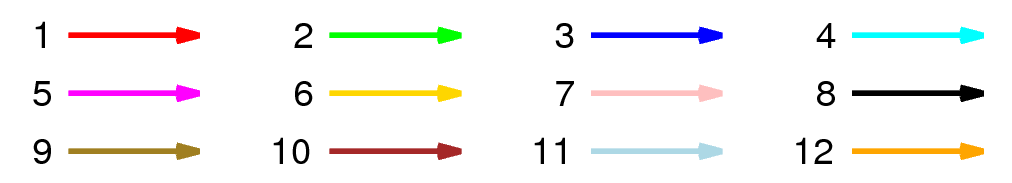
\includegraphics[width=16cm]{color.png} 
\end{center}
\begin{verbatim}
    1 -> red            2 -> green        3 -> blue           4 -> cyan
    5 -> magenta        6 -> gold         7 -> pink           8 -> black
    9 -> olive         10 -> brown       11 -> light-blue    12 -> orange
\end{verbatim} 
The number of each irreducible representation corresponds to its position
in the character table and is given below after the list of characters. 
Group of bands degenerate by time reversal might belong to a reducible
representation. In that case the bands are plotted with the color of the
irreducible represention with higher number contained in the decomposition
of the reducible representation.
The names of the irreducible representations have been taken from Ref.~[1]
for the point groups and from Ref.~[2] for the double point groups. 
The character tables of the $32$ point groups can be found in many places 
but the conventions and definitions can be slightly different. So in
this guide we include the tables as a reference even if there is some 
overlap with Ref.~[2]. The tables are those printed by the \qe\ 
routines. For each character only two digits are given, so the
following correspondence should be used:
$1.41 \rightarrow \sqrt{2}$, $1.73 \rightarrow \sqrt{3}$, 
$0.71 \rightarrow \sqrt{2}/2$, $0.87 \rightarrow \sqrt{3}/2$.
For the proper point groups or improper point groups isomorphic to a 
proper point group and for $S_6$ and $T_h$ all the projective 
representations are p-equivalent to the representations of the single 
or of the double point group.~[11] For the groups $C_{2h}$, $C_{4h}$, $C_{6h}$,
$D_{3d}$, and $O_h$ there is an additional nonequivalent projective 
set of representations, while for $D_{2h}$, $D_{4h}$, and $D_{6h}$ there 
are three additional projective sets that are reported in the tables below.
In a projective representation, elements belonging to the 
same class might have different characters so we report in the tables all 
the elements that have non-zero character (except for $O_h$ whose
projective table is given for groups of operations that have the same
non-zero character). 
Only one representative example of the many possible realizations of 
the point group is given. You can use the tool code 
\texttt{crystal\_point\_group.x} to have more precise information
on each point group. The names 
of these projective representations are taken from Ref.~[11] (and converted
to the name used in this manual for the representations of the point group 
and of the double point group) while the same color codes as described above 
are used for the projective representations (this feature is available
only in \texttt{thermo\_pw}).

The names of the symmetry operations are indicated using
the Sch\"onflies notation. 
We assume that the orientation of the axes is with the tip in the positive
$z$ hemisphere and positive rotation angles are counterclockwise about 
the rotation axis when seen from the tip to the origin. Axes in the $z=0$ 
plane are oriented with the tip in the
positive $x$ direction, and the $y$ axis is oriented in the 
direction of positive $y$. In this guide, improper rotations are described 
as rotations followed by inversion as in the Hermann-Mauguin (HM) 
definitions. In the Schoenflies notation improper rotations are rotations
followed by a mirror symmetry with respect to a plane perpendicular to 
the rotation axis.
So $S_6^5$ indicates a rotation of $+120^\circ$ degree about the axis 
followed by inversion (this operation is called $\bar 3$ in 
HM notation), $S_6$ a rotation of 
$-120^\circ$ followed by inversion ($\bar 3^5$), $S_3^5$ a rotation 
of $+60^\circ$ followed by inversion ($\bar 6$) and
$S_3$ a rotation of $-60^\circ$ followed by inversion ($\bar 6^5$).
$S_4^3$ is a rotation of $+90^\circ$ followed by inversion ($\bar 4$) and
$S_4$ is a rotation of $-90^\circ$ followed by inversion ($\bar 4^3$).
For the double groups a minus sign in front of the symmetry name
indicates that the operation is multiplied by the $360^\circ$ rotation 
(called \texttt{-E} in the tables or $\bar E$ in the text).

\newpage
\section{\color{coral}Point groups}

\subsection{\color{web-blue}$C_1\ (1)$}
This group contains only the identity ($E$) \texttt{[1]}. 
It is a group compatible with the triclinic Bravais lattice 
(\texttt{ibrav=14}). \\
Its Laue class is $C_i$. \\
The character table is:
\begin{verbatim}
C_1    E    
A      1.00       1
\end{verbatim}
There is only one irreducible representation, so all functions are 
totally symmetric. \\
The character table of the double group is ($\bar E$ indicates the
$360^\circ$ rotation): 
\begin{verbatim}
C_1    E     -E   
G_2    1.00 -1.00      1
\end{verbatim}
There is only one irreducible representation ($\Gamma_2$), 
so all functions are totally symmetric. \\
This group has no subgroup.

\newpage
\subsection{\color{web-blue}$C_i\ (\bar 1)$}
This group has two elements: The identity and inversion ($i$) \texttt{[28]}.
It is a group compatible with the triclinic Bravais lattice 
(\texttt{ibrav=14}). \\
Its Laue class is $C_i$. \\
The character table is:
\begin{verbatim}
C_i    E     i    
A_g    1.00  1.00      1
A_u    1.00 -1.00      1
\end{verbatim}
There are two representations distinguished by the parity
with respect to inversion: $A_g$ is even and $A_u$ is odd. \\
The character table of the double group is: 
\begin{verbatim}
C_i    E     -E    i     -i   
G_2+   1.00 -1.00  1.00 -1.00     1
G_2-   1.00 -1.00 -1.00  1.00     2
\end{verbatim}
There are two representations distinguished by the parity
with respect to inversion: $\Gamma_2^+$ is even and $\Gamma_2^-$ is odd.\\
$C_1$ is the only subgroup of $C_i$. The compatibility table for the
representations is:
\begin{verbatim}
C_i     A_u    A_g
C_1      A      A
\end{verbatim}
The compatibility table for the double group is:
\begin{verbatim}
C_i    G_2+   G_2- 
C_1    G_2    G_2
\end{verbatim}

\newpage
\subsection{\color{web-blue}$C_s\ (m)$}
This group has two elements: The identity and a mirror symmetry ($\sigma$).
It is a group compatible with the monoclinic system and with the
simple monoclinic (\texttt{ibrav=$\pm$12}) or the one-base centered monoclinic 
(\texttt{ibrav=$\pm$13}) Bravais lattices. \\
Its Laue class is $C_{2h}$. \\
The mirror plane can be perpendicular to several axes:  
$x$ \texttt{[17]}, $y$ \texttt{[16]}, $z$ \texttt{[15]}, 
$(x=y, z=0)$ \texttt{[18]}, 
$(x=-y, z=0)$ \texttt{[19]}, 
$(x=z, y=0)$ \texttt{[20]}, $(x=-z, y=0)$ \texttt{[21]},
$(y=z, x=0)$ \texttt{[22]}, $(y=-z, x=0)$ \texttt{[23]}, 
$(y=\sqrt{3}x, z=0)$ \texttt{[24]}, $(y=-\sqrt{3}x, z=0)$ \texttt{[25]}, 
$(y=x/\sqrt{3}, z=0)$ \texttt{[26]}, $(y=-x/\sqrt{3}, z=0)$ 
\texttt{[27]} ($x$ is a shorthand notation for
the axis $(y=0, z=0)$, $y$ is a shorthand notation for
the axis $(x=0, z=0)$, and $z$ is a shorthand notation for
the axis $(x=0, y=0)$). There are therefore $13$ 
realizations of interest for solids. \\
The character table is:
\begin{verbatim}
C_s    E     s
A'     1.00  1.00      1
A''    1.00 -1.00      2
\end{verbatim}
There are two representations distinguished by the parity
with respect to the mirror symmetry: $A'$ is even and $A''$ is odd.\\
The character table of the double group is:
\begin{verbatim}
     real part
C_s    E     -E    s     -s   
                              
G_3    1.00 -1.00  0.00  0.00       1 
G_4    1.00 -1.00  0.00  0.00       2

     imaginary part
       E     -E    s     -s   
G_3    0.00  0.00  1.00 -1.00       1
G_4    0.00  0.00 -1.00  1.00       2
\end{verbatim}
There are two one-dimensional representations distinguished by the 
behavior with respect to the mirror symmetry: the functions
are multiplied by $i$ according to $\Gamma_3$ and by
$-i$ according to $\Gamma_4$.\\
$C_1$ is the only subgroup of $C_i$. The compatibility table for the
representations is:
\begin{verbatim}
C_s     A'     A''
C_1     A      A
\end{verbatim}
The compatibility table for the double group is:
\begin{verbatim}
C_s    G_3    G_4 
C_1    G_2    G_2
\end{verbatim}

\newpage
\subsection{\color{web-blue}$C_2\ (2)$}
This group has two elements: The identity and a rotation of $180^\circ$ 
about an axis ($C_2$).
It is a group compatible with the monoclinic system and with the
simple monoclinic (\texttt{ibrav=$\pm$12}) or the one-base centered monoclinic 
(\texttt{ibrav=$\pm$13}) Bravais lattices. \\
Its Laue class is $C_{2h}$. \\
The axis can be:  
$x$ \texttt{[4]}, $y$ \texttt{[3]}, $z$ \texttt{[2]}, 
$(x=y, z=0)$ \texttt{[5]}, $(x=-y, z=0)$ \texttt{[6]}, 
$(x=z, y=0)$ \texttt{[7]}, 
$(x=-z, y=0)$ \texttt{[8]},
$(y=z, x=0)$ \texttt{[9]}, $(y=-z, x=0)$ \texttt{[10]}, 
$(y=\sqrt{3}x, z=0)$ \texttt{[12]}, $(y=-\sqrt{3}x, z=0)$ \texttt{[11]}, 
$(y=x/\sqrt{3}, z=0)$ \texttt{[14]}, $(y=-x/\sqrt{3}, z=0)$ \texttt{[13]}. 
There are therefore $13$ realizations of interest for solids. \\
The character table is:
\begin{verbatim}
C_2    E     C2
A      1.00  1.00    1
B      1.00 -1.00    2
\end{verbatim}
There are two representations distinguished by the parity
with respect to the rotation: $A$ is even and $B$ is odd.\\
The character table of the double group is:
\begin{verbatim}
     real part
C_2    E     -E    C2    -C2
G_3    1.00 -1.00  0.00  0.00     1
G_4    1.00 -1.00  0.00  0.00     2

     imaginary part
       E     -E    C2    -C2
G_3    0.00  0.00  1.00 -1.00     1
G_4    0.00  0.00 -1.00  1.00     2
\end{verbatim}
There are two one-dimensional representations distinguished by the 
behavior with respect to the rotation: the functions
are multiplied by $i$ according to $\Gamma_3$ and by $-i$ according to 
$\Gamma_4$.\\
$C_1$ is the only subgroup of $C_2$. \\
The compatibility table is:
\begin{verbatim}
C_2     A      B  
C_1     A      A
\end{verbatim}
The compatibility table for the double group is:
\begin{verbatim}
C_2    G_3    G_4 
C_1    G_2    G_2
\end{verbatim}

\newpage
\subsection{\color{web-blue}$C_3\ (3)$}
This group has three elements: The identity and two rotations of $\pm120^\circ$ 
about an axis ($C_3$ and $C_3^2$).
It is a group compatible with the trigonal and hexagonal systems and with the
rhombohedral (\texttt{ibrav=5}) or the hexagonal (\texttt{ibrav=4}) Bravais 
lattices. \\
Its Laue class is $S_6$. \\
The $C_3$ axis can be: $z$ \texttt{[33]}, $x=y=z$ \texttt{[29]}, 
$x=-y=z$ \texttt{[32]}, $x=-y=-z$ \texttt{[30]}, $x=y=-z$ \texttt{[31]}.
There are therefore $5$ realizations of interest for solids. \\
The character table is:
\begin{verbatim}
     real part
C_3    E     C3    C3^2
A      1.00  1.00  1.00      1
E      1.00 -0.50 -0.50      2
E*     1.00 -0.50 -0.50      3

     imaginary part
A      0.00  0.00  0.00      1
E      0.00  0.87 -0.87      2
E*     0.00 -0.87  0.87      3 
\end{verbatim}
There are three one-dimensional representations: $A$ is totally symmetric, while
a $C_3$ rotation multiplies the functions by $e^{i\phi}$ according to $E$
and by $e^{-i\phi}$ according to $E^*$ ($\phi=2 \pi / 3$). \\
The character table of the double group is:
\begin{verbatim}
     real part
C_3    E     -E    C3    -C3   C3^2  -C3^2
G_4    1.00 -1.00  0.50 -0.50  0.50 -0.50     1
G_5    1.00 -1.00  0.50 -0.50  0.50 -0.50     2
G_6    1.00 -1.00 -1.00  1.00 -1.00  1.00     3

     imaginary part
       E     -E    C3    -C3   C3^2  -C3^2
G_4    0.00  0.00  0.87 -0.87 -0.87  0.87     1
G_5    0.00  0.00 -0.87  0.87  0.87 -0.87     2
G_6    0.00  0.00  0.00  0.00  0.00  0.00     3
\end{verbatim}
There are three irreducible representations that can be distinguished by the
behavior in a $C_3$ rotation: the functions are multiplied by $e^{i\phi/2}$ according
to $\Gamma_4$, by $e^{-i\phi/2}$ according to $\Gamma_5$ and by $e^{i\pi}=-1$ 
according to $\Gamma_6$ ($\phi=2 \pi / 3$). \\
$C_1$ is the only subgroup of $C_3$. \\
The compatibility table is:
\begin{verbatim}
C_3     A      E      E*  
C_1     A      A      A
\end{verbatim}
The compatibility table for the double group is:
\begin{verbatim}
C_3    G_4    G_5    G_6 
C_1    G_2    G_2    G_2
\end{verbatim}

\newpage
\subsection{\color{web-blue}$C_4\ (4)$}
This group has four elements: The identity, two rotations of $\pm90^\circ$ 
about an axis ($C_4$ and $C_4^3$), and a rotation of $180^\circ$ about the same
axis ($C_2$).
It is a group compatible with the tetragonal system and with the
simple tetragonal (\texttt{ibrav=6}) or centered tetragonal (\texttt{ibrav=7})
Bravais lattices. \\ 
Its Laue class is $C_{4h}$. \\
The axes can be: $x$ \texttt{[36]}, $y$ \texttt{[35]}, or $z$ \texttt{[34]}.
There are therefore $3$ realizations of interest for solids. \\
The character table is:
\begin{verbatim}
     real part
C_4    E     C4    C2    C4^3
A      1.00  1.00  1.00  1.00       1
B      1.00 -1.00  1.00 -1.00       2
E      1.00  0.00 -1.00  0.00       3
E*     1.00  0.00 -1.00  0.00       4

     imaginary part
       E     C4    C2    C4^3
A      0.00  0.00  0.00  0.00       1
B      0.00  0.00  0.00  0.00       2
E      0.00  1.00  0.00 -1.00       3
E*     0.00 -1.00  0.00  1.00       4
\end{verbatim}
There are four irreducible representations that can be distinguished according
to the behavior for a $C_4$ rotations. $A$ is totally symmetric, while for a
$C_4$ rotation the functions are multiplied by $e^{i\pi}=-1$ according to 
$B$, by $e^{i\pi/2}=i$ according to $E$ and by $e^{-i\pi/2}=-i$ according to
$E^*$. \\
The character table of the double group is:
\begin{verbatim}
     real part
C_4    E     -E    C4    -C4   C2    -C2   C4^3  -C4^3
G_5    1.00 -1.00  0.71 -0.71  0.00  0.00  0.71 -0.71      1
G_6    1.00 -1.00  0.71 -0.71  0.00  0.00  0.71 -0.71      2
G_7    1.00 -1.00 -0.71  0.71  0.00  0.00 -0.71  0.71      3
G_8    1.00 -1.00 -0.71  0.71  0.00  0.00 -0.71  0.71      4

     imaginary part
       E     -E    C4    -C4   C2    -C2   C4^3  -C4^3
G_5    0.00  0.00  0.71 -0.71  1.00 -1.00 -0.71  0.71      1
G_6    0.00  0.00 -0.71  0.71 -1.00  1.00  0.71 -0.71      2
G_7    0.00  0.00 -0.71  0.71  1.00 -1.00  0.71 -0.71      3
G_8    0.00  0.00  0.71 -0.71 -1.00  1.00 -0.71  0.71      4
\end{verbatim}
There are four irreducible representations distinguished according
to the behavior for a $C_4$ rotation. The functions are multiplied by 
$e^{i\omega}$ according to $\Gamma_5$, by $-e^{i3\omega}$ according to 
$\Gamma_6$, by $-e^{i\omega}$ according to $\Gamma_7$, and by $e^{i3\omega}$ 
according to $\Gamma_8$ ($\omega=\pi/4$). Note that this table has some
differences both with Ref.~[2] and Ref.~[8].\\
$C_4$ has two subgroups $C_1$ and $C_2$. The $C_2$ subgroup has the same axis
as $C_4$. \\
The compatibility table is:
\begin{verbatim}
C_4     A      B      E      E*  
C_1     A      A      A      A
C_2     A      A      B      B
\end{verbatim}
The compatibility table for the double group is:
\begin{verbatim}
C_4     G_5    G_6    G_7    G_8 
C_1     G_2    G_2    G_2    G_2
C_2     G_3    G_4    G_3    G_4
\end{verbatim}

\newpage
\subsection{\color{web-blue}$C_6\ (6)$}
This group has six elements: The identity, two rotations of $\pm60^\circ$ 
about an axis ($C_6$ and $C_6^5$), two rotations of $\pm120^\circ$
about the same axis ($C_3$ and $C_3^2$) and a rotation of $180^\circ$ about 
the same axis ($C_2$).
It is a group compatible with the hexagonal system and with the
hexagonal (\texttt{ibrav=4}) Bravais lattice. \\ 
Its Laue class is $C_{6h}$. \\
The $C_6$ axis is $z$ \texttt{[37]}.
There is therefore $1$ realization of interest for solids. \\
The character table is:
\begin{verbatim}
     real part
C_6    E     C6    C3    C2    C3^2  C6^5 
A      1.00  1.00  1.00  1.00  1.00  1.00       1
B      1.00 -1.00  1.00 -1.00  1.00 -1.00       2
E_1    1.00  0.50 -0.50 -1.00 -0.50  0.50       3 
E_1*   1.00  0.50 -0.50 -1.00 -0.50  0.50       4
E_2    1.00 -0.50 -0.50  1.00 -0.50 -0.50       5
E_2*   1.00 -0.50 -0.50  1.00 -0.50 -0.50       6

     imaginary part
       E     C6    C3    C2    C3^2  C6^5 
A      0.00  0.00  0.00  0.00  0.00  0.00       1
B      0.00  0.00  0.00  0.00  0.00  0.00       2
E_1    0.00  0.87  0.87  0.00 -0.87 -0.87       3
E_1*   0.00 -0.87 -0.87  0.00  0.87  0.87       4
E_2    0.00  0.87 -0.87  0.00  0.87 -0.87       5
E_2*   0.00 -0.87  0.87  0.00 -0.87  0.87       6
\end{verbatim}
There are six irreducible representations distinguished for
the behavior for a $C_6$ rotation. $A$ is totally symmetric, while
the functions are multiplied by $e^{i\pi}=-1$ according
to $B$, by $e^{i\psi}$ according to $E_1$, by $e^{-i\psi}$ 
according to $E_1^*$, by $e^{i2\psi}$ according to $E_2$, and by $e^{-i2\psi}$
according to $E_2^*$ ($\psi=\pi/3$). \\
The character table of the double group is:
\begin{verbatim}
     real part
C_6  E     -E    C6    -C6   C3    -C3   C2    -C2   C3^2  -C3^2 C6^5  -C6^5
G_7  1.00 -1.00  0.87 -0.87  0.50 -0.50  0.00  0.00  0.50 -0.50  0.87 -0.87  1
G_8  1.00 -1.00  0.87 -0.87  0.50 -0.50  0.00  0.00  0.50 -0.50  0.87 -0.87  2
G_9  1.00 -1.00 -0.87  0.87  0.50 -0.50  0.00  0.00  0.50 -0.50 -0.87  0.87  3  
G_10 1.00 -1.00 -0.87  0.87  0.50 -0.50  0.00  0.00  0.50 -0.50 -0.87  0.87  4
G_11 1.00 -1.00  0.00  0.00 -1.00  1.00  0.00  0.00 -1.00  1.00  0.00  0.00  5
G_12 1.00 -1.00  0.00  0.00 -1.00  1.00  0.00  0.00 -1.00  1.00  0.00  0.00  6

     imaginary part
     E     -E    C6    -C6   C3    -C3   C2    -C2   C3^2  -C3^2 C6^5  -C6^5
G_7  0.00  0.00  0.50 -0.50  0.87 -0.87  1.00 -1.00 -0.87  0.87 -0.50  0.50  1
G_8  0.00  0.00 -0.50  0.50 -0.87  0.87 -1.00  1.00  0.87 -0.87  0.50 -0.50  2
G_9  0.00  0.00 -0.50  0.50  0.87 -0.87 -1.00  1.00 -0.87  0.87  0.50 -0.50  3
G_10 0.00  0.00  0.50 -0.50 -0.87  0.87  1.00 -1.00  0.87 -0.87 -0.50  0.50  4
G_11 0.00  0.00  1.00 -1.00  0.00  0.00 -1.00  1.00  0.00  0.00 -1.00  1.00  5
G_12 0.00  0.00 -1.00  1.00  0.00  0.00  1.00 -1.00  0.00  0.00  1.00 -1.00  6
\end{verbatim}
There are six irreducible representations distinguished for the
behavior for a $C_6$ rotation. The functions are multiplied
by $e^{i\psi/2}$ according to $\Gamma_7$, by $-e^{i5\psi/2}$ 
according to $\Gamma_8$,
by $-e^{-i\psi/2}$ according to $\Gamma_9$, $e^{i5\psi/2}$ 
according to $\Gamma_{10}$,
by $e^{i3\psi/2}=i$ according to $\Gamma_{11}$, and $-e^{i3\psi/2}=-i$ according 
to $\Gamma_{12}$ ($\psi=\pi/3$). \\
The subgroups of $C_6$ are $C_1$, $C_2$, and $C_3$. Both $C_2$ and $C_3$ have
the rotation axis coinciding with the $C_6$ axis of $C_6$. \\
The compatibility table is:
\begin{verbatim}
C_6     A      B      E_1    E_1*   E_2   E_2* 
C_1     A      A      A      A      A     A
C_2     A      B      B      B      A     A
C_3     A      A      E      E*     E*    E
\end{verbatim}
The compatibility table for the double group is:
\begin{verbatim}
C_6     G_7    G_8    G_9    G_10   G_11   G_12 
C_1     G_2    G_2    G_2    G_2    G_2    G_2
C_2     G_3    G_4    G_4    G_3    G_4    G_3
C_3     G_4    G_5    G_4    G_5    G_6    G_6
\end{verbatim}

\newpage
\subsection{\color{web-blue}$D_2\ (222)$ or $V$} 
This group has four elements: The identity and three rotations of $180^\circ$ about 
three perpendicular axes ($C_2$, $C_2'$, and $C_2''$). It is a group compatible with 
the orthorhombic system and with the simple orthorhombic (\texttt{ibrav=8}), 
the one-face centered orthorhombic (\texttt{ibrav=9}), the face-centered orthorhombic 
(\texttt{ibrav=10}), and the body-centered orthorhombic (\texttt{ibrav=11}) Bravais 
lattices. \\ 
Its Laue class is $D_{2h}$. \\
The three perpendicular axes can be: 
\begin{itemize}
\item
a) $z$ ($C_2$), $x$ ($C_2'$), and $y$ ($C_2''$) \texttt{[38]}
\item
b) $x$ ($C_2$), ($y=z$, $x=0$) ($C_2'$), ($y=-z$, $x=0$) ($C_2''$) \texttt{[41]}
\item
c) $y$ ($C_2$), ($x=-z$, $y=0$) ($C_2'$), ($x=z$, $y=0$) ($C_2''$) \texttt{[40]}
\item
d) $z$ ($C_2$), ($y=-x$, $z=0$) ($C_2'$), ($y=x$, $z=0$) ($C_2''$) \texttt{[39]}
\item
e) $z$ ($C_2$), ($y=-x/\sqrt{3}$, $z=0$) ($C_2'$), ($y=\sqrt{3}x$, $z=0$) ($C_2''$) \texttt{[42]}
\item
f) $z$ ($C_2$), ($y=-\sqrt{3}x$, $z=0$) ($C_2'$), ($y=x/\sqrt{3}$, $z=0$) ($C_2''$) \texttt{[43]}
\end{itemize}
There are therefore $6$ realizations of interest in solids. \\
The character table is:
\begin{verbatim}
D_2    E     C2    C2'   C2''
A      1.00  1.00  1.00  1.00    1
B_1    1.00  1.00 -1.00 -1.00    2
B_2    1.00 -1.00  1.00 -1.00    3
B_3    1.00 -1.00 -1.00  1.00    4
\end{verbatim}
There are four one-dimensional irreducible representations.
$A$ is totally symmetric, $B_1$ is even with respect to
$C_2$ and odd with respect to $C_2'$ and $C_2''$, 
$B_2$ is even with respect to $C_2'$ and odd with respect to $C_2$ or $C_2''$,
and $B_3$ is even with respect to $C_2''$ and odd with respect to
$C_2$ or $C_2'$. \\
The character table of the double group is:
\begin{verbatim}
D_2    E     -E    C2    C2'   C2'' 
                   -C2   -C2'  -C2''
G_5    2.00 -2.00  0.00  0.00  0.00     1
\end{verbatim}
There is only one irreducible representation. \\
The subgroups of $D_2$ are $C_1$ and $C_2$. The axis of $C_2$ can be parallel to
any of the three axes of $D_2$ and therefore there are three lines in the
compatibility table for the cases in which the axis of $C_2$ is parallel to 
$C_2$ (case 1), $C_2'$ (case 2) or $C_2''$ (case 3). 
The compatibility table is:
\begin{verbatim}
D_2     A      B_1    B_2    B_3  
C_1     A      A      A      A   
C_2_1   A      A      B      B     
C_2_2   A      B      A      B   
C_2_3   A      B      B      A
\end{verbatim}
The compatibility table for the double group does not distinguish the different
cases:
\begin{verbatim}
D_2     G_5  
C_1     2 G_2
C_2     G_3 + G_4
\end{verbatim}

\newpage
\subsection{\color{web-blue}$D_3\ (32)$}
This group has six elements: The identity, two rotations of $\pm120^\circ$ about
an axis ($C_3$ and $C_3^2$) and three rotations of $180^\circ$ 
($3C_2'$) about three axes perpendicular to the axis of $C_3$.
It is a group compatible with the trigonal and hexagonal systems and with the
rhombohedral (\texttt{ibrav=5}) and hexagonal (\texttt{ibrav=4})
Bravais lattices. \\ 
Its Laue class is $D_{3d}$. \\
The $C_3$ axis can be: $z$, $x=y=z$, $x=-y=z$, $x=-y=-z$, $x=y=-z$.
When the $C_3$ axis is $z$, the three $C_2'$ axes can be
$x$, $(y=\sqrt{3}x, z=0)$, $(y=-\sqrt{3}x, z=0)$ \texttt{[44]} or 
$y$, $(y=x/\sqrt{3}, z=0)$, $(y=-x/\sqrt{3}, z=0)$ \texttt{[45]}. 
When the $C_3$ axis is $x=y=z$ the three $C_2'$ axes are
($y=-z$, $x=0$), ($x=-y$, $z=0$), ($x=-z$, $y=0$) \texttt{[46]}.
When the $C_3$ axis is $x=-y=z$ the three $C_2'$ axes are
($y=z$, $x=0$), ($x=-z$, $y=0$), ($x=y$, $z=0$) \texttt{[47]}.
When the $C_3$ axis is $x=-y=-z$ the three $C_2'$ axes are
($x=z$, $y=0$), ($x=y$, $z=0$), ($y=-z$, $x=0$) \texttt{[48]}.
When the $C_3$ axis is $x=y=-z$ the three $C_2'$ axes are
($x=z$, $y=0$), ($y=z$, $x=0$), ($x=-y$, $z=0$) \texttt{[48]}. 
There are therefore $6$ realizations of interest for solids. \\
The character table is:
\begin{verbatim}
D_3    E     2C3   3C2'
A_1    1.00  1.00  1.00      1
A_2    1.00  1.00 -1.00      2
E      2.00 -1.00  0.00      3
\end{verbatim}
There are three irreducible representations. $A_1$ is totally symmetric,
$E$ is two-fold degenerate and $A_2$ is odd with respect to the
$C_2'$ rotations.\\
The character table of the double group is:
\begin{verbatim}
    real part
D_3    E     -E    2C3   -2C3   3C2' -3C2'
G_4    2.00 -2.00  1.00 -1.00  0.00  0.00      1
G_5    1.00 -1.00 -1.00  1.00  0.00  0.00      2
G_6    1.00 -1.00 -1.00  1.00  0.00  0.00      3

     imaginary part
       E     -E    2C3   -2C3   3C2' -3C2'
G_4    0.00  0.00  0.00  0.00  0.00  0.00      1
G_5    0.00  0.00  0.00  0.00  1.00 -1.00      2
G_6    0.00  0.00  0.00  0.00 -1.00  1.00      3
\end{verbatim}
There are three irreducible representations. $\Gamma_4$ is two-dimensional,
while $\Gamma_5$ and $\Gamma_6$ which are both one dimensional can be distinguished
because for a $C_2'$ rotation the functions are multiplied by $i$ according to
$\Gamma_5$ and by $-i$ according to $\Gamma_6$. \\
The subgroups of $D_3$ are $C_1$, $C_2$, and $C_3$. The $C_2$ axis is 
parallel to one of the $C_2'$ axes of $D_3$, while the $C_3$ axis 
of $C_3$ is parallel to the $C_3$ axis of $D_3$. \\
The compatibility table is:
\begin{verbatim}
D_3     A_1    A_2    E    
C_1     A      A      2 A      
C_2     A      B      A + B        
C_3     A      A      E + E*      
\end{verbatim}
The compatibility table for the double group is:
\begin{verbatim}
D_3     G_4          G_5    G_6    
C_1     2 G_2        G_2    G_2
C_2     G_3 + G_4    G_3    G_4
C_3     G_4 + G_5    G_6    G_6   
\end{verbatim}

\newpage
\subsection{\color{web-blue}$D_4\ (422)$} 
This group has eight elements: The identity, two rotations of 
$\pm90^\circ$ about
an axis ($C_4$ and $C_4^3$), a rotation of $180^\circ$ about the same axis and
four rotations of $180^\circ$ ($2C_2'$ and $2C_2''$) about axes perpendicular 
to the $C_4$ axis. It is a group compatible with the tetragonal system and with the
simple tetragonal (\texttt{ibrav=6}) and centered tetragonal (\texttt{ibrav=7})
Bravais lattices. \\ 
Its Laue class is $D_{4h}$. \\
The $C_4$ axis can be: $x$, $y$, or $z$. The four $C_2$ perpendicular rotation
axes are: 
\begin{itemize}
\item
a) $C_4$ coinciding with $x$: $y$, $z$ ($C_2'$), ($y=\pm z$, $x=0$) ($C_2''$)
\texttt{[52]}.
\item
b) $C_4$ coinciding with $y$: $x$, $z$ ($C_2'$), ($x=\pm z$, $y=0$) ($C_2''$)
\texttt{[51]}.
\item
c) $C_4$ coinciding with $z$: $x$, $y$ ($C_2'$), ($y=\pm x$, $z=0$) ($C_2''$)
\texttt{[50]}.
\end{itemize}
There are therefore $3$ realizations of interest for solids. \\
The character table is:
\begin{verbatim}
D_4    E     2C4   C2    2C2'  2C2''
A_1    1.00  1.00  1.00  1.00  1.00      1
A_2    1.00  1.00  1.00 -1.00 -1.00      2
B_1    1.00 -1.00  1.00  1.00 -1.00      3
B_2    1.00 -1.00  1.00 -1.00  1.00      4
E      2.00  0.00 -2.00  0.00  0.00      5
\end{verbatim}
There are five irreducible representations. $A_1$ is totally symmetric 
and $E$ is two-fold degenerate. The other representations can be distinguished
according to the behavior with respect to the $C_2'$ and $C_2''$ rotations.
$A_2$ is odd with respect to both $C_2'$ and $C_2''$, $B_1$ is even with respect
to $C_2'$ and odd with respect to $C_2''$, while $B_2$ is odd with respect to
$C_2'$ and even with respect to $C_2''$. \\ 
The character table of the double group is:
\begin{verbatim}
D_4    E     -E    2C4   -2C4   C2   2C2'  2C2''
                               -C2   -2C2' -2C2''
G_6    2.00 -2.00  1.41 -1.41  0.00  0.00  0.00      1
G_7    2.00 -2.00 -1.41  1.41  0.00  0.00  0.00      2
\end{verbatim}
There are two two-fold degenerate irreducible representations that can be 
distinguished for the character with respect to a $C_4$ rotation, equal
to $\sqrt{2}$ according to $\Gamma_6$ and to $-\sqrt{2}$ according to $\Gamma_7$. \\
The subgroups of $D_4$ are $C_1$, $C_2$, $C_4$, and $D_2$. 
The axis of $C_2$ can coincide with the $C_4$ axis of $D_4$ (case 1), 
with a $C_2'$ axis (case 2) or with a $C_2''$ axis (case 3). 
The axis of $C_4$ coincides with the $C_4$ axis of $D_4$.
The axis $C_2$ of $D_2$ can coincide with the $C_4$ axis
of $D_4$ while the $C_2'$ and $C_2''$ axes of $D_2$ can coincide with the $C_2'$
axes of $D_4$ (case 1) or with the $C_2''$ axes of $D_4$ (case 2), 
or the axis $C_2'$ of $D_2$ coincides with the $C_4$ axis
of $D_4$ while the $C_2$ and $C_2''$ axes of $D_2$ coincide with the $C_2'$
axes of $D_4$ (case 3), or the axis $C_2''$ of $D_2$ coincides with the $C_4$ axis
of $D_4$ while the $C_2$ and $C_2'$ axes of $D_2$ coincide with the $C_2'$
axes of $D_4$ (case 4). The two cases in which $C_2'$ is parallel to the
$C_4$ axis of $D_4$ and $C_2$ and $C_2''$ are parallel to the $C_2''$ axes of
$D_4$, or $C_2''$ is parallel to the $C_4$ axis of $D_4$ and
$C_2$ and $C_2'$ are parallel to the $C_2''$ axes of $D_4$ are 
excluded by the choice of axes of $D_2$. When only one axis of $D_2$
is parallel to $x$, $y$, or $z$ that axis is always $C_2$. \\
The compatibility table is:
\begin{verbatim}
D_4      A_1    A_2    B_1     B_2      E
C_1       A      A      A       A      2 A
C_2_1     A      A      A       A      2 B
C_2_2     A      B      A       B     A + B
C_2_3     A      B      B       A     A + B
C_4       A      A      B       B     E + E*      
D_2_1     A      B_1    A       B_1   B_2 + B_3
D_2_2     A      B_1    B_1     A     B_2 + B_3
D_2_3     A      B_2    A       B_2   B_1 + B_3
D_2_4     A      B_3    A       B_3   B_1 + B_2
\end{verbatim}
The compatibility table for the double group is:
\begin{verbatim}
D_4     G_6             G_7  
C_1     G_2             G_2   
C_2     G_3 + G_4       G_3 + G_4   
C_4     G_5 + G_6       G_7 + G_8
D_2     G_5             G_5
\end{verbatim}

\newpage
\subsection{\color{web-blue}$D_6\ (622)$} 
This group has twelve elements: The identity, two rotations of 
$\pm60^\circ$ about an axis ($C_6$ and $C_6^5$), two rotations of 
$\pm120^\circ$ about the same axis
($C_3$ and $C_3^2$), a rotation of $180^\circ$ about the same axis and
six rotations of $180^\circ$ ($3C_2'$ and $3C_2''$) about axes perpendicular 
to the $C_6$ axis \texttt{[53]}. It is a group compatible with the 
hexagonal system and with the
hexagonal (\texttt{ibrav=4}) Bravais lattice. \\ 
Its Laue class is $D_{6h}$. \\
The $C_6$ axis is the $z$ axis. The six $C_2$ perpendicular rotation axes are
$x$, ($y=\pm\sqrt{3}x$, $z=0$) ($C_2'$), 
$y$, ($y=\pm x/\sqrt{3}$, $z=0$) ($C_2''$). There is therefore
$1$ realization of interest for solids. \\
The character table is:
\begin{verbatim}
D_6    E     2C6   2C3   C2    3C2'  3C2''
A_1    1.00  1.00  1.00  1.00  1.00  1.00      1
A_2    1.00  1.00  1.00  1.00 -1.00 -1.00      2
B_1    1.00 -1.00  1.00 -1.00  1.00 -1.00      3
B_2    1.00 -1.00  1.00 -1.00 -1.00  1.00      4
E_1    2.00  1.00 -1.00 -2.00  0.00  0.00      5
E_2    2.00 -1.00 -1.00  2.00  0.00  0.00      6
\end{verbatim}
There are six irreducible representations. $A_1$ is totally symmetric.
$A_2$, $B_1$, and $B_2$ are one dimensional and can be distinguished for the
behavior with respect to the $C_2'$ and $C_2''$ rotations. $A_2$ is odd 
with respect to both rotations, $B_1$ is even with respect to $C_2'$ and 
odd with respect to $C_2''$ while $B_2$ is odd with respect to $C_2'$ and
even with respect to $C_2''$. $E_1$ and $E_2$ are both two dimensional and
can be distinguished for the character with respect to the $C_2$ 
rotation. It is $-2$ for $E_1$ and $2$ for $E_2$. \\
The character table for the double group is:
\begin{verbatim}
D_6    E     -E     2C6  -2C6   2C3  -2C3   C2    3C2' 3C2''
                                           -C2   -3C2' -3C2''
G_7    2.00 -2.00  1.73 -1.73  1.00 -1.00  0.00  0.00  0.00     1
G_8    2.00 -2.00 -1.73  1.73  1.00 -1.00  0.00  0.00  0.00     2
G_9    2.00 -2.00  0.00  0.00 -2.00  2.00  0.00  0.00  0.00     3
\end{verbatim}
There are three irreducible representations, all two dimensional. 
They can be distinguished for the character with respect to the $C_6$ rotation.
It is $\sqrt{3}$ according to $\Gamma_7$, $-\sqrt{3}$ according to $\Gamma_8$ 
and $0$ according to $\Gamma_9$.\\
The subgroups of $D_6$ are $C_1$, $C_2$, $C_3$, $C_6$, $D_2$, and $D_3$. 
The axis of $C_2$ can coincide with the $C_6$ axis (case 1), with a $C_2'$ axis 
of $D_6$ (case 2) or with a $C_2''$ axis of $D_6$ (case 3). 
The axes of $C_3$ and $C_6$ coincide with the $C_6$ axis of $D_6$. 
The $C_2$ axis of $D_2$ coincides with the 
$C_6$ axis of $D_6$, the $C_2'$ axis of $D_2$ coincides with a $C_2'$ axis of $D_6$,
while the $C_2''$ axis of $D_2$ coincides with a $C_2''$ axis of $D_6$. 
The $C_3$ axis of $D_3$ coincides with the $C_6$ axis of $D_6$ and the $C_2'$ axes
of $D_3$ can coincide with the $C_2'$ axes of $D_6$ (case 1) or with the
$C_2''$ axes of $D_6$ (case 2).\\
The compatibility table is:
\begin{verbatim}
D_6     A_1    A_2    B_1     B_2      E_1        E_2
C_1     A      A       A       A       2 A        2 A
C_2_1   A      A       B       B       2 B        2 A
C_2_2   A      B       A       B      A + B      A + B
C_2_3   A      B       B       A      A + B      A + B
C_3     A      A       A       A      E + E*     E + E*      
C_6     A      A       B       B     E_1+E_1*   E_2+E_2*   
D_2     A      B_1     B_2     B_3   B_2+B_3     A + B_1
D_3_1   A_1    A_2     A_1     A_2      E          E
D_3_2   A_1    A_2     A_2     A_1      E          E
\end{verbatim}
The compatibility table for the double group is:
\begin{verbatim}
D_6      G_7          G_8           G_9 
C_1    2 G_2        2 G_2         2 G_2
C_2    G_3 + G_4    G_3 + G_4     G_3 + G_4
C_3    G_4 + G_5    G_4 + G_5     2 G_6
C_6    G_7 + G_8    G_9 + G_10    G_11 + G_12
D_2       G_5          G_5           G_5
D_3       G_4          G_4        G_5 + G_6
\end{verbatim}

\newpage
\subsection{\color{web-blue}$C_{2v}\ (mm2)$} 
This group has four elements: The identity, a rotation of $180^\circ$ about
an axis ($C_2$) and two mirror planes ($\sigma_v$ and $\sigma_v'$) that contain 
the $C_2$ axis.
It is a group compatible with the orthorhombic system and with the
simple orthorhombic (\texttt{ibrav=8}), the one-base centered
orthorhombic (\texttt{ibrav=9}), the face-centered orthorhombic 
(\texttt{ibrav=10}), and the body-centered orthorhombic (\texttt{ibrav=11}) 
Bravais lattices.\\
Its Laue class is $D_{2h}$. \\
The $C_2$ axis can be:
$x$, $y$, $z$, $(x=y, z=0)$, $(x=-y, z=0)$, $(x=z, y=0)$, $(x=-z, y=0)$,
$(y=z, x=0)$, $(y=-z, x=0)$, $(y=x/\sqrt{3}, z=0)$, $(y=-x/\sqrt{3}, z=0)$, 
$(y=\sqrt{3}x, z=0)$, $(y=-\sqrt{3}x, z=0)$. For the mirror planes there are
the following possibilities:
\begin{verbatim}
         C_2                perp. to s_v           perp. to s_v'
a)        x                      y                      z          [54]
b)        x                 y=z,     x=0           y=-z,    x=0    [55]
c)        y                      z                      x          [56]
d)        y                 x=-z,    y=0           x=z,     y=0    [57]
e)        z                      x                      y          [58]    
f)        z                 x=-y,    z=0           x=y,     z=0    [59]
g)   x=y,    z=0                 z                 x=-y,    z=0    [60]
h)   x=-y,   z=0            x=y      z=0                z          [61] 
i)   x=z,    y=0                 y                 x=-z,    y=0    [62] 
l)   x=-z,   y=0            x=z,     y=0                y          [63]
m)   y=z,    x=0            y=-z,    x=0                x          [64]
n)   y=-z,   x=0                 x                 y=z,     x=0    [65]
o)        z                 y=-m x,  z=0           y=x/m,   z=0    [66] 
p)        z                 y=-x/m,  z=0           y= m x,  z=0    [67] 
q)   y=x/m,  z=0                 z                 y=-m x,  z=0    [68]
r)   y=-x/m, z=0            y= m x,  z=0                z          [69]
s)   y= m x, z=0                 z                 y=-x/m,  z=0    [70]
t)   y=-m x, z=0            y= x/m,  z=0                z          [71]
\end{verbatim}
where $m=\sqrt{3}$.
There are therefore $18$ realizations of interest for solids. \\
The character table is (isomorphic to $D_2$ with $C_2 \rightarrow C_2$,
$\sigma_v \rightarrow C_2'$, $\sigma_v' \rightarrow C_2''$):
\begin{verbatim}
C_2v   E     C2    s_v    s_v'
A_1    1.00  1.00  1.00  1.00      1
A_2    1.00  1.00 -1.00 -1.00      2
B_1    1.00 -1.00  1.00 -1.00      3
B_2    1.00 -1.00 -1.00  1.00      4
\end{verbatim}
There are four irreducible representations. $A_1$ is totally symmetric while
$A_2$ is odd with respect to both mirror symmetries.  
$B_1$ is even with respect to the mirror $\sigma_v$ and odd with respect to
the mirror $\sigma_v'$, while $B_2$ is odd with respect to $\sigma_v$ and even 
with respect to $\sigma_v'$. In order to fully characterize $B_1$ and $B_2$
it is important to make a definite choice for the planes $\sigma_v$ and $\sigma_v'$.
We use the definition in the previous table. Therefore even or odd is with respect
to the mirror planes given in this table. \\
The character table of the double group is:
\begin{verbatim}
C_2v   E     -E     C2    s_v   s_v'
                   -C2   -s_v  -s_v'
G_5    2.00 -2.00  0.00  0.00  0.00     1
\end{verbatim}
There is only one irreducible representation $\Gamma_5$. \\
The subgroups of $C_{2v}$ are $C_1$, $C_s$, and $C_2$. The axis of $C_2$ is 
parallel to the $C_2$ axis of $C_{2v}$, while the mirror of $C_s$ can coincide
with $\sigma_v$ (case 1) or with $\sigma_v'$ (case 2). \\
The compatibility table is:
\begin{verbatim}
C_2v    A_1      A_2       B_1       B_2
C_1      A        A         A         A
C_s_1    A'       A''       A'        A''
C_s_2    A'       A''       A''       A'
C_2      A        A         B         B
\end{verbatim}
The compatibility table for the double group is:
\begin{verbatim}
C_2v     G_5
C_1     2 G_2
C_s     G_3 + G_4
C_2     G_3 + G_4
\end{verbatim}

\newpage
\subsection{\color{web-blue}$C_{3v}\ (3m)$} 
This group has six elements: The identity, two rotations of $\pm120^\circ$ about
an axis ($C_3$ and $C_3^2$) and three mirror planes ($3\sigma_v$) 
that contain the $C_3$ axis.
It is a group compatible with the trigonal and hexagonal systems and with the  
rhombohedral (\texttt{ibrav=5}) and hexagonal (\texttt{ibrav=4}) Bravais lattices. \\ 
Its Laue class is $D_{3d}$. \\
The $C_3$ axis can be: $z$, $x=y=z$, $x=-y=z$, $x=-y=-z$, $x=y=-z$.
For the mirror planes there are the following possibilities:
\begin{verbatim}
      C_3        perp. to s_v       perp to s_v'     perp to s_v''
a)     z             x              y=m x, z=0       y=-m x, z=0     [72]
b)     z         y=x/m, z=0              y           y=-x/m, z=0     [73]
c)    x=y=z      y=-z  x=0          x=-y,  z=0       x=-z,   y=0     [74]
d)    x=-y=z     y=z,  x=0          x=-z,  y=0       x=y,    z=0     [75]
e)    x=-y=-z    x=z,  y=0          x=y,   z=0       y=-z,   x=0     [76]
f)    x=y=-z     x=z,  y=0          y=z,   x=0       x=-y,   z=0     [77]
\end{verbatim}
There are therefore $6$ realizations of interest for solids. \\
The character table is (isomorphic to $D_3$ with $\sigma_v \rightarrow C_2$):
\begin{verbatim}
C_3v   E     2C3   3s_v
A_1    1.00  1.00  1.00      1
A_2    1.00  1.00 -1.00      2
E      2.00 -1.00  0.00      3
\end{verbatim}
There are three irreducible representations and since the three mirror planes
are in the same class the choice of $\sigma_v$, $\sigma_v'$, or $\sigma_v''$ is
irrelevant to distinguish the representations. $A_1$ is totally symmetric,
$A_2$ is odd with respect to the mirror symmetries and $E$ is two dimensional. \\
The character table of the double group is:
\begin{verbatim}
     real part
C_3v   E     -E    2C3   -2C3  3s_v  -3s_v
G_4    2.00 -2.00  1.00 -1.00  0.00  0.00      1
G_5    1.00 -1.00 -1.00  1.00  0.00  0.00      2
G_6    1.00 -1.00 -1.00  1.00  0.00  0.00      3

     imaginary part
       E     -E    2C3   -2C3  3s_v  -3s_v
G_4    0.00  0.00  0.00  0.00  0.00  0.00      1
G_5    0.00  0.00  0.00  0.00  1.00 -1.00      2
G_6    0.00  0.00  0.00  0.00 -1.00  1.00      3
\end{verbatim}
There are three irreducible representations. $\Gamma_4$ is two dimensional, while
$\Gamma_5$ and $\Gamma_6$ can be distinguished because for a mirror symmetry the
functions are multiplied by $i$ according to $\Gamma_5$ and by $-i$ according to
$\Gamma_6$. \\
The subgroups of $C_{3v}$ are $C_1$, $C_s$, and $C_3$. The axis of $C_3$ coincides
with the axis of $C_{3v}$, while the mirror plane of $C_s$ coincides with
one of the three mirrors of $C_{3v}$. \\
The compatibility table is:
\begin{verbatim}
C_3v    A_1      A_2      E
C_1      A        A       A
C_s      A'       A''    A' + A''
C_3      A        A      E  + E*
\end{verbatim}
The compatibility table for the double group is:
\begin{verbatim}
C_3v    G_4        G_5      G_6
C_1     2 G_2      G_2      G_2
C_s    G_3 + G_4   G_3      G_4
C_3    G_4 + G_5   G_6      G_6
\end{verbatim}

\newpage
\subsection{\color{web-blue}$C_{4v}\ (4mm)$} 
This group has eight elements: The identity, two rotations of $\pm90^\circ$ 
about an axis ($C_4$ and $C_4^3$), a rotation of $180^\circ$ about the same axis 
($C_2$) and four mirror symmetries ($2\sigma_v$ and $2 \sigma_d$) with respect
to planes that contain the $C_4$ axis.
It is a group compatible with the tetragonal system and with the  
simple tetragonal \texttt{ibrav=6}) and centered tetragonal (\texttt{ibrav=7}) 
Bravais lattices. \\ 
Its Laue class is $D_{4h}$. \\
The $C_4$ axis can be: $x$, $y$, $z$. When the $C_4$ axis is $x$ the axes
perpendicular to the mirror planes are $(y=\pm z, x=0)$ ($\sigma_v$), 
$y$, $z$ ($\sigma_d$) \texttt{[80]}. When the $C_4$ axis is $y$
the axes perpendicular to the mirror planes are $x$, $z$ ($\sigma_v$),
$(x=\pm z, y=0)$ ($\sigma_d$) \texttt{[79]}. When the 
$C_4$ axis is $z$ the axes perpendicular to the mirror planes are $x$, $y$
($\sigma_v$), $(y=\pm x, z=0)$ ($\sigma_d$) \texttt{[78]}.
There are therefore $3$ realizations of interest for solids. \\
The character table is (isomorphic to $D_4$ with $\sigma_v \rightarrow C_2'$
and $\sigma_d \rightarrow C_2''$):
\begin{verbatim}
C_4v   E     2C4   C2    2s_v  2s_d 
A_1    1.00  1.00  1.00  1.00  1.00       1
A_2    1.00  1.00  1.00 -1.00 -1.00       2
B_1    1.00 -1.00  1.00  1.00 -1.00       3
B_2    1.00 -1.00  1.00 -1.00  1.00       4
E      2.00  0.00 -2.00  0.00  0.00       5
\end{verbatim}
There are 5 irreducible representations. $A_1$ is totally symmetric, $E$ is
two dimensional and $A_2$ is odd with respect to all mirror symmetries.
To distinguish $B_1$ and $B_2$ we have to fix the mirror planes
$\sigma_v$ and $\sigma_d$ as written above. 
The representation $B_1$ is even with respect to the mirror symmetries
$\sigma_v$ and odd with respect to $\sigma_d$, while $B_2$ is odd with respect to
$\sigma_v$ and even with respect to $\sigma_d$. \\
The character table of the double group is:
\begin{verbatim}
C_4v   E     -E    2C4   -2C4   C2    2s_v  2s_d
                               -C2   -2s_v -2s_d
G_6    2.00 -2.00  1.41 -1.41  0.00  0.00  0.00      1
G_7    2.00 -2.00 -1.41  1.41  0.00  0.00  0.00      2
\end{verbatim}
There are two irreducible representations, both two dimensional. They can be
distinguished from the character for a $C_4$ rotation. It is
$\sqrt{2}$ according to $\Gamma_6$ and $-\sqrt{2}$ with respect to 
$\Gamma_7$. \\
The subgroups of $C_{4v}$ are $C_1$, $C_s$, $C_2$, $C_4$, and C$_{2v}$. 
The axes of $C_2$, $C_4$, and $C_{2v}$ coincide with the axis of $C_{4v}$, 
while the mirror plane of $C_s$ coincides with a $\sigma_v$ 
(case 1) or with a $\sigma_d$ (case 2). Similarly the two
mirror planes of $C_{2v}$ can coincide with the two planes $\sigma_v$ 
(case 1) or with the two planes $\sigma_d$ (case 2).\\
The compatibility table is:
\begin{verbatim}
C_4v    A_1      A_2      B_1       B_2       E
C_1      A        A        A        A        2 A
C_s_1    A'       A''      A'       A''    A' + A''
C_s_2    A'       A''      A''      A'     A' + A''
C_2      A        A        A        A        2 B
C_4      A        A        B        B      E  + E*   
C_2v_1   A_1      A_2      A_1      A_2   B_1 + B_2
C_2v_2   A_1      A_2      A_2      A_1   B_1 + B_2
\end{verbatim}
The compatibility table of the double group is:
\begin{verbatim}
C_4v    G_6          G_7  
C_1    2 G_2        2 G_2
C_s    G_3 + G_4    G_3 + G_4
C_2    G_3 + G_4    G_3 + G_4
C_4    G_5 + G_6    G_7 + G_8
C_2v    G_5          G_5
\end{verbatim}

\newpage
\subsection{\color{web-blue}$C_{6v}\ (6mm)$} 
This group has twelve elements: The identity, two rotations of $\pm60^\circ$ 
about an axis ($C_6$ and $C_6^5$), two rotations of $\pm120^\circ$
about the same axis ($C_3$ and $C_3^2$), a rotation of $180^\circ$ about 
the same axis ($C_2$), and six mirror symmetries with respect to
planes ($3\sigma_v$ and $3\sigma_d$) that contain the $C_6$ axis \texttt{[81]}.
It is a group compatible with the hexagonal system and with the  
hexagonal (\texttt{ibrav=4}) Bravais lattice. \\ 
Its Laue class is $D_{6h}$. \\
The $C_6$ axis is the $z$ axis. The mirror planes $\sigma_v$ are perpendicular 
to $y$ and to $(y=\pm x/\sqrt{3}, z=0)$, while the mirror planes $\sigma_d$
are perpendicular to $x$ and to $(y=\pm \sqrt{3} x, z=0)$.
There is therefore $1$ realization of interest for solids. \\
The character table is (isomorphic to $D_6$ with $\sigma_d \rightarrow C_2'$
and $\sigma_v \rightarrow C_2''$):
\begin{verbatim}
C_6v   E     2C6   2C3   C2    3s_d  3s_v 
A_1    1.00  1.00  1.00  1.00  1.00  1.00      1
A_2    1.00  1.00  1.00  1.00 -1.00 -1.00      2
B_1    1.00 -1.00  1.00 -1.00  1.00 -1.00      3
B_2    1.00 -1.00  1.00 -1.00 -1.00  1.00      4
E_1    2.00  1.00 -1.00 -2.00  0.00  0.00      5
E_2    2.00 -1.00 -1.00  2.00  0.00  0.00      6
\end{verbatim}
There are six irreducible representations. $A_1$ is totally symmetric, while
$A_2$ is odd with respect to all mirror symmetries. $B_1$ and $B_2$ can be
distinguished for the behaviour for a $\sigma_v$ and a
$\sigma_d$ reflection. $B_1$ is even with respect to the planes $\sigma_d$
and odd with respect to the planes $\sigma_v$, while $B_2$ is odd with
respect to the planes $\sigma_d$ and even with respect to the planes 
$\sigma_v$. $E_1$ and $E_2$ are both two dimensional and can be 
distinguished by the character of a $C_6$ rotation. It is
$1$ according to $E_1$ and $-1$ according to $E_2$.\\
The character table of the double group is:
\begin{verbatim}
C_6v   E     -E     2C6  -2C6   2C3  -2C3   C2    3s_d  3s_v
                                           -C2   -3s_d -3s_v
G_7    2.00 -2.00  1.73 -1.73  1.00 -1.00  0.00  0.00  0.00    1
G_8    2.00 -2.00 -1.73  1.73  1.00 -1.00  0.00  0.00  0.00    2
G_9    2.00 -2.00  0.00  0.00 -2.00  2.00  0.00  0.00  0.00    3
\end{verbatim}
There are three two-dimensional irreducible representations that can be 
distinguished for the character of the $C_6$ rotations, equal to $\sqrt{3}$
according to $\Gamma_7$, to $-\sqrt{3}$ according to $\Gamma_8$ and to
$0$ according to $\Gamma_9$.\\
The subgroups of $C_{6v}$ are $C_1$, $C_s$, $C_2$, $C_3$, $C_6$,
$C_{2v}$, and $C_{3v}$. The rotation axes of $C_2$, $C_3$, $C_6$, $C_{2v}$,
and $C_{3v}$ coincide with the rotation axis of $C_{6v}$. The mirror 
plane of $C_s$ can be a $\sigma_d$ (case 1) or a $\sigma_v$ (case 2). The two 
mirror planes of $C_{2v}$
can coincide with the two planes perpendicular to $x$ and $y$, 
or perpendicular to $(y=\sqrt{3} x, z=0)$ and $(y=-x /\sqrt{3}, z=0)$,
or perpendicular to $(y=-\sqrt{3} x, z=0)$ and $(y=x /\sqrt{3}, z=0)$.
There are therefore two possibilities. The plane $\sigma_v$ of $C_{2v}$
can coincide with one of the planes $\sigma_d$ (case 1) of $C_{2v}$
or with one of the planes $\sigma_v$ (case 2).
The three mirror planes of $C_{3v}$ can coincide with the three mirrors 
$\sigma_d$ of $C_{6v}$ (case 1) or with the three mirrors $\sigma_v$ (case 2).\\
The compatibility table is:
\begin{verbatim}
C_6v    A_1      A_2      B_1       B_2      E_1           E_2
C_1      A        A        A         A       2 A           2 A
C_s_1    A'       A''      A'        A''    A' + A''     A' + A''
C_s_2    A'       A''      A''       A'     A' + A''     A' + A''
C_2      A        A        B         B       2 B           2 A
C_3      A        A        A         A      E  + E*      E  + E*
C_6      A        A        B         B     E_1 + E_1*   E_2 + E_2*
C_2v_1   A_1      A_2      B_1       B_2   B_1 + B_2    A_1 + A_2
C_2v_2   A_1      A_2      B_2       B_1   B_1 + B_2    A_1 + A_2
C_3v_1   A_1      A_2      A_1       A_2       E            E  
C_3v_2   A_1      A_2      A_2       A_1       E            E
\end{verbatim}
The compatibility table for the double group is:
\begin{verbatim}
C_6v    G_7          G_8             G_9
C_1    2 G_2        2 G_2           2 G_2
C_s    G_3 + G_4    G_3 + G_4      G_3 + G_4
C_2    G_3 + G_4    G_3 + G_4      G_3 + G_4
C_3    G_4 + G_5    G_4 + G_5       2 G_6
C_6    G_7 + G_8    G_9 + G_10     G_11 + G_12
C_2v    G_5          G_5             G_5
C_3v    G_4          G_4           G_5 + G_6
\end{verbatim}

\newpage
\subsection{\color{web-blue}$C_{2h}\ (2/m)$} 
This group has four elements: The identity, a rotation of $180^\circ$ 
about an axis ($C_2$), inversion and a mirror symmetry with respect to 
a plane perpendicular to the $C_2$ axis.
It is a group compatible with the monoclinic system and with the  
simple monoclinic (\texttt{ibrav=$\pm$12}) and one-base centered monoclinic
(\texttt{ibrav=$\pm$13}) Bravais lattices. \\ 
Its Laue class is $C_{2h}$. \\
The axis can be:
$x$ \texttt{[84]}, $y$ \texttt{[83]}, $z$ \texttt{[82]}, 
$(x=y, z=0)$ \texttt{[85]}, $(x=-y, z=0)$ \texttt{[86]}, 
$(x=z, y=0)$ \texttt{[87]}, $(x=-z, y=0)$ \texttt{[88]},
$(y=z, x=0)$ \texttt{[89]}, 
$(y=-z, x=0)$ \texttt{[90]}, $(y=\sqrt{3}x, z=0)$ \texttt{[91]}, 
$(y=-\sqrt{3}x, z=0)$ \texttt{[92]},
$(y=x/\sqrt{3}, z=0)$ \texttt{[93]}, 
$(y=-x/\sqrt{3}, z=0)$ \texttt{[94]}. The mirror plane $\sigma_h$ 
is perpendicular to the axis. There are therefore $13$ realizations 
of interest for solids. \\
The character table is (using $C_{2h}=C_2 \times C_i$):
\begin{verbatim}
C_2h   E     C2    i     s_h
A_g    1.00  1.00  1.00  1.00       1
B_g    1.00 -1.00  1.00 -1.00       2
A_u    1.00  1.00 -1.00 -1.00       3
B_u    1.00 -1.00 -1.00  1.00       4
\end{verbatim}
There are four irreducible representations, two even $A_g$ and $B_g$ and
two odd $A_u$ and $B_u$ with respect to inversion. $A$ and $B$ representations
are distinguished by the fact that $A$ are even with respect
to the $C_2$ rotation and $B$ are odd. \\
The character table of the double group is:
\begin{verbatim}
     real part
C_2h   E     -E    C2    -C2   i     -i    s_h   -s_h 
G_3+   1.00 -1.00  0.00  0.00  1.00 -1.00  0.00  0.00     1
G_4+   1.00 -1.00  0.00  0.00  1.00 -1.00  0.00  0.00     2
G_3-   1.00 -1.00  0.00  0.00 -1.00  1.00  0.00  0.00     3
G_4-   1.00 -1.00  0.00  0.00 -1.00  1.00  0.00  0.00     4

     imaginary part
       E     -E    C2    -C2   i     -i    s_h   -s_h 
G_3+   0.00  0.00  1.00 -1.00  0.00  0.00  1.00 -1.00     1
G_4+   0.00  0.00 -1.00  1.00  0.00  0.00 -1.00  1.00     2
G_3-   0.00  0.00  1.00 -1.00  0.00  0.00 -1.00  1.00     3
G_4-   0.00  0.00 -1.00  1.00  0.00  0.00  1.00 -1.00     4
\end{verbatim}
There are four one-dimensional irreducible representations. $\Gamma_3^+$
and $\Gamma_4^+$ are even with respect to inversion, while
$\Gamma_3^-$ and $\Gamma_4^-$ are odd. $\Gamma_3$ and $\Gamma_4$ 
representations can be distinguished because for the $C_2$ rotation
the functions are multiplied by $i$ according to $\Gamma_3$ and 
by $-i$ according to $\Gamma_4$. \\
The subgroups of $C_{2h}$ are $C_1$, $C_i$, $C_s$, and $C_2$. The
axis of $C_2$ coincides with the axis of $C_{2h}$, while the 
mirror of $C_s$ coincides with the mirror of $C_{2h}$.\\
The compatibility table is:
\begin{verbatim}
C_2h     A_g      B_g     A_u     B_u
C_1       A        A       A       A
C_i      A_g      A_g     A_u     A_u
C_s       A'       A''     A''     A'
C_2       A        B       A       B
\end{verbatim}
The compatibility table of the double group is:
\begin{verbatim}
C_2h     G_3+      G_4+     G_3-     G_4- 
C_1      G_2       G_2      G_2      G_2
C_i      G_2+      G_2+     G_2-     G_2-
C_s      G_3       G_4      G_4      G_3
C_2      G_3       G_4      G_3      G_4
\end{verbatim}
This group has also projective representations corresponding to
$IC_2 = \beta C_2 I$ and $\beta=-1$ ($I$ is the inversion).
With the representations of the $C_2$ point group one can build [11]:
\begin{verbatim}
     real part
C_2h      E     
BA      2.00       1
\end{verbatim}
With the representations of the $C_2$ double point group we have:
\begin{verbatim}
     real part
C_2h      E     
G_4G_3  2.00       1
\end{verbatim}
All elements not explicitely indicated have zero character.

\newpage
\subsection{\color{web-blue}$C_{3h}\ (\bar 6)$}  
This group has six elements: The identity, two rotation of $\pm120^\circ$ 
about an axis ($C_3$ and $C_3^2$), a mirror symmetry with respect to a 
plane perpendicular to the $C_3$ axis and the product of these operations, 
that is rotations of $\pm60^\circ$ multiplied by inversion 
($S_3^5$ and $S_3$) \texttt{[95]}.
It is a group compatible with the hexagonal system and with the  
hexagonal (\texttt{ibrav=4}) Bravais lattice. \\ 
Its Laue class is $C_{6h}$. \\
The $C_3$ axis must be parallel to the $z$ axis. There is therefore
$1$ realization of interest for solids. \\
The character table is (using $C_{3h}=C_3 \times \sigma_h$):
\begin{verbatim}
     real part
C_3h   E     C3    C3^2  s_h   S3    S3^5 
A'     1.00  1.00  1.00  1.00  1.00  1.00      1
E'     1.00 -0.50 -0.50  1.00 -0.50 -0.50      2
E'*    1.00 -0.50 -0.50  1.00 -0.50 -0.50      3
A''    1.00  1.00  1.00 -1.00 -1.00 -1.00      4
E''    1.00 -0.50 -0.50 -1.00  0.50  0.50      5
E''*   1.00 -0.50 -0.50 -1.00  0.50  0.50      6

     imaginary part
       E     C3    C3^2  s_h   S3    S3^5 
A'     0.00  0.00  0.00  0.00  0.00  0.00      1
E'     0.00  0.87 -0.87  0.00  0.87 -0.87      2
E'*    0.00 -0.87  0.87  0.00 -0.87  0.87      3
A''    0.00  0.00  0.00  0.00  0.00  0.00      4
E''    0.00  0.87 -0.87  0.00 -0.87  0.87      5
E''*   0.00 -0.87  0.87  0.00  0.87 -0.87      6
\end{verbatim}
The group has six irreducible representations. The representation 
$A'$, $E'$, and $E'^*$ are even with respect to the mirror symmetry, while
$A''$, $E''$, and $E''^*$ are odd. The representations $A$, $E$, and $E*$
can be distinguished for the behavior for a $C_3$ rotation. 
The functions are multiplied by $1$ according to $A$, by $e^{i\phi}$ according to 
$E$ representations and by $e^{-i\phi}$ according to $E^*$ ($\phi=\pi /3$). \\
The character table of the double group is:
\begin{verbatim}
     real part
C_3h  E     -E    C3    -C3   C3^2  -C3^2  s_h  -s_h   S3   -S3   S3^5 -S3^5
G_7   1.00 -1.00  0.50 -0.50  0.50 -0.50  0.00  0.00  0.87 -0.87  0.87 -0.87 1
G_8   1.00 -1.00  0.50 -0.50  0.50 -0.50  0.00  0.00  0.87 -0.87  0.87 -0.87 2
G_9   1.00 -1.00  0.50 -0.50  0.50 -0.50  0.00  0.00 -0.87  0.87 -0.87  0.87 3
G_10  1.00 -1.00  0.50 -0.50  0.50 -0.50  0.00  0.00 -0.87  0.87 -0.87  0.87 4
G_11  1.00 -1.00 -1.00  1.00 -1.00  1.00  0.00  0.00  0.00  0.00  0.00  0.00 5
G_12  1.00 -1.00 -1.00  1.00 -1.00  1.00  0.00  0.00  0.00  0.00  0.00  0.00 6

     imaginary part
      E     -E    C3    -C3   C3^2  -C3^2  s_h  -s_h   S3   -S3   S3^5 -S3^5
G_7   0.00  0.00  0.87 -0.87 -0.87  0.87  1.00 -1.00 -0.50  0.50  0.50 -0.50 1
G_8   0.00  0.00 -0.87  0.87  0.87 -0.87 -1.00  1.00  0.50 -0.50 -0.50  0.50 2
G_9   0.00  0.00  0.87 -0.87 -0.87  0.87 -1.00  1.00  0.50 -0.50 -0.50  0.50 3
G_10  0.00  0.00 -0.87  0.87  0.87 -0.87  1.00 -1.00 -0.50  0.50  0.50 -0.50 4
G_11  0.00  0.00  0.00  0.00  0.00  0.00 -1.00  1.00 -1.00  1.00  1.00 -1.00 5
G_12  0.00  0.00  0.00  0.00  0.00  0.00  1.00 -1.00  1.00 -1.00 -1.00  1.00 6
\end{verbatim}
There are six one-dimensional irreducible representations that can be
distinguished for the behavior for a $S_3^5$ operation. The functions
are multiplied by $e^{i\psi/2}$ according to $\Gamma_7$, by $-e^{i5\psi/2}$
according to $\Gamma_8$, by $-e^{i\psi/2}$ according to $\Gamma_9$,
by $e^{i5\psi/2}$ according to $\Gamma_{10}$, $e^{-i3\psi/2}=-i$ according
according to $\Gamma_{11}$, $e^{i3\psi/2}=i$ according to $\Gamma_{12}$
($\psi=\pi/3$).\\
The subgroups of $C_{3h}$ are $C_1$, $C_s$, and $C_3$. The axis of $C_3$
coincides with the rotation axis of $C_{3h}$, while the mirror of $C_s$ coincides
with the mirror $\sigma_h$ of $C_{3h}$. \\ 
The compatibility table is:
\begin{verbatim}
C_3h     A'        E'       E'*      A''        E''        E''* 
C_1      A         A        A        A          A          A
C_s      A'        A'       A'       A''        A''        A''
C_3      A         E        E*       A          E          E*
\end{verbatim}
The compatibility table of the double group is:
\begin{verbatim}
C_3h     G_7      G_8      G_9      G_10      G_11      G_12
C_1      G_2      G_2      G_2      G_2       G_2       G_2
C_s      G_3      G_4      G_4      G_3       G_4       G_3
C_3      G_4      G_5      G_4      G_5       G_6       G_6
\end{verbatim}

\newpage
\subsection{\color{web-blue}$C_{4h}\ (4/m)$}  
This group has eight elements: The identity, two rotation of $\pm90^\circ$ 
about an axis ($C_4$ and $C_4^3$), a rotation of $180^\circ$ about the
same axis ($C_2$), inversion, and the product of inversion with previous
rotations that gives two rotations of $\pm90^\circ$ multiplied by inversion 
($S_4^3$ and $S_4$) and a mirror symmetry $\sigma_h$ with respect to a plane 
perpendicular to the $C_4$ axis.  
It is a group compatible with the tetragonal system and with the  
simple tetragonal (\texttt{ibrav=6}) and centered tetragonal (\texttt{ibrav=7})
Bravais lattices. \\ 
Its Laue class is $C_{4h}$. \\
The $C_4$ axis can be parallel to $x$ \texttt{[98]}, $y$ \texttt{[97]}, 
or $z$ \texttt{[96]}. There are therefore
$3$ realizations of interest for solids. \\
The character table is (using $C_{4h}=C_4 \times C_i$):
\begin{verbatim}
     real part
C_4h   E     C4    C2    C4^3  i     S4^3  s_h   S4   
A_g    1.00  1.00  1.00  1.00  1.00  1.00  1.00  1.00      1
B_g    1.00 -1.00  1.00 -1.00  1.00 -1.00  1.00 -1.00      2
E_g    1.00  0.00 -1.00  0.00  1.00  0.00 -1.00  0.00      3
E_g*   1.00  0.00 -1.00  0.00  1.00  0.00 -1.00  0.00      4
A_u    1.00  1.00  1.00  1.00 -1.00 -1.00 -1.00 -1.00      5
B_u    1.00 -1.00  1.00 -1.00 -1.00  1.00 -1.00  1.00      6
E_u    1.00  0.00 -1.00  0.00 -1.00  0.00  1.00  0.00      7
E_u*   1.00  0.00 -1.00  0.00 -1.00  0.00  1.00  0.00      8

     imaginary part
       E     C4    C2    C4^3  i     S4^3  s_h   S4   
A_g    0.00  0.00  0.00  0.00  0.00  0.00  0.00  0.00      1
B_g    0.00  0.00  0.00  0.00  0.00  0.00  0.00  0.00      2
E_g    0.00  1.00  0.00 -1.00  0.00  1.00  0.00 -1.00      3
E_g*   0.00 -1.00  0.00  1.00  0.00 -1.00  0.00  1.00      4
A_u    0.00  0.00  0.00  0.00  0.00  0.00  0.00  0.00      5
B_u    0.00  0.00  0.00  0.00  0.00  0.00  0.00  0.00      6
E_u    0.00  1.00  0.00 -1.00  0.00 -1.00  0.00  1.00      7
E_u*   0.00 -1.00  0.00  1.00  0.00  1.00  0.00 -1.00      8
\end{verbatim}
There are eight irreducible representations. $A_g$, $B_g$, $E_g$, and
$E_g^*$ are even with respect to inversion while $A_u$, $B_u$, $E_u$,
and $E_u^*$ are odd. $A$, $B$, $E$, and $E^*$ can be recognized for the
behavior for a $C_4$ rotation. The functions are multiplied by 
$1$ according to $A$ representations, by $-1$ according to $B$,
by $i$ according to $E$ and by $-i$ according to $E^*$. \\
The character table for the double group is:
\begin{verbatim}
     real part
C_4h   E     -E    C4    -C4   C2    -C2   C4^3  -C4^3 i     -i    S4^3  -S4^3
G_5+   1.00 -1.00  0.71 -0.71  0.00  0.00  0.71 -0.71  1.00 -1.00  0.71 -0.71
G_6+   1.00 -1.00  0.71 -0.71  0.00  0.00  0.71 -0.71  1.00 -1.00  0.71 -0.71
G_7+   1.00 -1.00 -0.71  0.71  0.00  0.00 -0.71  0.71  1.00 -1.00 -0.71  0.71
G_8+   1.00 -1.00 -0.71  0.71  0.00  0.00 -0.71  0.71  1.00 -1.00 -0.71  0.71
G_5-   1.00 -1.00  0.71 -0.71  0.00  0.00  0.71 -0.71 -1.00  1.00 -0.71  0.71
G_6-   1.00 -1.00  0.71 -0.71  0.00  0.00  0.71 -0.71 -1.00  1.00 -0.71  0.71
G_7-   1.00 -1.00 -0.71  0.71  0.00  0.00 -0.71  0.71 -1.00  1.00  0.71 -0.71
G_8-   1.00 -1.00 -0.71  0.71  0.00  0.00 -0.71  0.71 -1.00  1.00  0.71 -0.71

       s_h   -s_h  S4    -S4  
G_5+   0.00  0.00  0.71 -0.71     1
G_6+   0.00  0.00  0.71 -0.71     2
G_7+   0.00  0.00 -0.71  0.71     3
G_8+   0.00  0.00 -0.71  0.71     4
G_5-   0.00  0.00 -0.71  0.71     5
G_6-   0.00  0.00 -0.71  0.71     6
G_7-   0.00  0.00  0.71 -0.71     7
G_8-   0.00  0.00  0.71 -0.71     8

     imaginary part
       E     -E    C4    -C4   C2    -C2   C4^3  -C4^3 i     -i    S4^3  -S4^3
G_5+   0.00  0.00  0.71 -0.71  1.00 -1.00 -0.71  0.71  0.00  0.00  0.71 -0.71
G_6+   0.00  0.00 -0.71  0.71 -1.00  1.00  0.71 -0.71  0.00  0.00 -0.71  0.71
G_7+   0.00  0.00 -0.71  0.71  1.00 -1.00  0.71 -0.71  0.00  0.00 -0.71  0.71
G_8+   0.00  0.00  0.71 -0.71 -1.00  1.00 -0.71  0.71  0.00  0.00  0.71 -0.71
G_5-   0.00  0.00  0.71 -0.71  1.00 -1.00 -0.71  0.71  0.00  0.00 -0.71  0.71
G_6-   0.00  0.00 -0.71  0.71 -1.00  1.00  0.71 -0.71  0.00  0.00  0.71 -0.71
G_7-   0.00  0.00 -0.71  0.71  1.00 -1.00  0.71 -0.71  0.00  0.00  0.71 -0.71
G_8-   0.00  0.00  0.71 -0.71 -1.00  1.00 -0.71  0.71  0.00  0.00 -0.71  0.71

       s_h   -s_h  S4    -S4  
G_5+   1.00 -1.00 -0.71  0.71     1
G_6+  -1.00  1.00  0.71 -0.71     2
G_7+   1.00 -1.00  0.71 -0.71     3
G_8+  -1.00  1.00 -0.71  0.71     4
G_5-  -1.00  1.00  0.71 -0.71     5
G_6-   1.00 -1.00 -0.71  0.71     6
G_7-  -1.00  1.00 -0.71  0.71     7
G_8-   1.00 -1.00  0.71 -0.71     8

\end{verbatim}
There are eight irreducible representations. $\Gamma_5^+$, $\Gamma_6^+$,
$\Gamma_7^+$, and $\Gamma_8^+$ are even with respect to inversion, while
$\Gamma_5^-$, $\Gamma_6^-$, $\Gamma_7^-$, and $\Gamma_8^-$ are odd.
The representations $\Gamma_5$, $\Gamma_6$, $\Gamma_7$, and $\Gamma_8$ can
be distinguished according to the behavior for a $C_4$ rotation. The
functions are multiplied by $e^{i\omega}$ according to $\Gamma_5$,
$-e^{i3\omega}$ according to $\Gamma_6$, by $-e^{i\omega}$ according to
$\Gamma_7$, and by $e^{i3\omega}$ according to $\Gamma_8$.\\
The subgroups of $C_{4h}$ are $C_1$, $C_i$, $C_s$, $C_2$, $C_4$, $C_{2h}$,
and $S_4$.  The axes of $C_2$, $C_4$, $C_{2h}$, and $S_4$
coincide with the $C_4$ axis of $C_{4h}$.
The mirror $\sigma$ of $C_s$ coincides with the mirror $\sigma_h$ of $C_{4h}$. \\
The compatibility table is:
\begin{verbatim}
C_4h     A_g    B_g    E_g    E_g^*    A_u    B_u    E_u     E_u^*
C_1      A      A      A       A        A      A      A       A
C_i      A_g    A_g    A_g    A_g      A_u    A_u    A_u     A_u
C_s      A'     A'     A''    A''       A''    A''    A'      A'
C_2      A      A      B      B         A      A      B       B
C_4      A      B      E      E*        A      B      E       E*
C_2h     A_g    A_g    B_g    B_g       A_u    A_u    B_u     B_u
S_4      A      B      E      E*        B      A      E*      E 
\end{verbatim}
The compatibility table for the double group is:
\begin{verbatim}
C_4h     G_5+    G_6+   G_7+   G_8+    G_5-   G_6-    G_7-    G_8-
C_1      G_2     G_2    G_2    G_2     G_2    G_2     G_2     G_2
C_i      G_2+    G_2+   G_2+   G_2+    G_2-   G_2-    G_2-    G_2-     
C_s      G_3     G_4    G_3    G_4     G_4    G_3     G_4     G_3
C_2      G_3     G_4    G_3    G_4     G_3    G_4     G_3     G_4
C_4      G_5     G_6    G_7    G_8     G_5    G_6     G_7     G_8
C_2h     G_3+    G_4+   G_3+   G_4+    G_3-   G_4-    G_3-    G_4-
S_4      G_5     G_6    G_7    G_8     G_7    G_8     G_5     G_6
\end{verbatim}
This group has also projective representations corresponding to
$I 4z = \beta 4z I$ and $\beta=-1$ ($I$ is the inversion).
With the representations of the $C_4$ point group one can obtain [11]:
\begin{verbatim}
     real part
C_4h      E         2z
E* E     2.00     -2.00     1
BA       2.00      2.00     2
     imaginary part
C_4h      E         2z
E* E     0.00      0.00     1
BA       0.00      0.00     2
\end{verbatim}
With the representations of the $C_4$ double point group we have:
\begin{verbatim}
     real part
C_4h      E         2z
G_6G_8   2.00      0.00     1
G_7G_5   2.00      0.00     2
     imaginary part
C_4h      E         2z
G_6G_8   0.00     -2.00     1
G_7G_5   0.00      2.00     2
\end{verbatim}
All elements not explicitely indicated have zero character.

\newpage
\subsection{\color{web-blue}$C_{6h}\ (6/m)$}  
This group has twelve elements: The identity, two rotations of $\pm60^\circ$ 
about an axis ($C_6$ and $C_6^5$), two rotations of $\pm120^\circ$
about the same axis ($C_3$ and $C_3^2$), a rotation of $180^\circ$ about the
same axis ($C_2$), inversion, and the product of inversion with previous
rotations that gives two rotations of $\pm60^\circ$ multiplied by inversion
($S_3^5$ and $S_3$), two rotations of $\pm120^\circ$ multiplied 
by inversion ($S_6^5$ and $S_6$), and a mirror $\sigma_h$
with respect to a plane perpendicular to the $C_6$ axis \texttt{[99]}. 
It is a group compatible with the hexagonal system and with the  
hexagonal (\texttt{ibrav=4}) Bravais lattice. \\ 
Its Laue class is $C_{6h}$. \\
The $C_6$ axis is parallel to the $z$ axis. There is therefore
$1$ realization of interest for solids. \\
The character table is (using $C_{6h}=C_6 \times C_i$):
\begin{verbatim}
    real part
C_6h E     C6    C3    C2    C3^2  C6^5  i     S3^5  S6^5  s_h   S6    S3   
A_g  1.00  1.00  1.00  1.00  1.00  1.00  1.00  1.00  1.00  1.00  1.00  1.00  1
B_g  1.00 -1.00  1.00 -1.00  1.00 -1.00  1.00 -1.00  1.00 -1.00  1.00 -1.00  2
E_1g 1.00  0.50 -0.50 -1.00 -0.50  0.50  1.00  0.50 -0.50 -1.00 -0.50  0.50  3
E1g* 1.00  0.50 -0.50 -1.00 -0.50  0.50  1.00  0.50 -0.50 -1.00 -0.50  0.50  4
E_2g 1.00 -0.50 -0.50  1.00 -0.50 -0.50  1.00 -0.50 -0.50  1.00 -0.50 -0.50  5
E2g* 1.00 -0.50 -0.50  1.00 -0.50 -0.50  1.00 -0.50 -0.50  1.00 -0.50 -0.50  6
A_u  1.00  1.00  1.00  1.00  1.00  1.00 -1.00 -1.00 -1.00 -1.00 -1.00 -1.00  7
B_u  1.00 -1.00  1.00 -1.00  1.00 -1.00 -1.00  1.00 -1.00  1.00 -1.00  1.00  8
E_1u 1.00  0.50 -0.50 -1.00 -0.50  0.50 -1.00 -0.50  0.50  1.00  0.50 -0.50  9
E1u* 1.00  0.50 -0.50 -1.00 -0.50  0.50 -1.00 -0.50  0.50  1.00  0.50 -0.50 10
E_2u 1.00 -0.50 -0.50  1.00 -0.50 -0.50 -1.00  0.50  0.50 -1.00  0.50  0.50 11
E2u* 1.00 -0.50 -0.50  1.00 -0.50 -0.50 -1.00  0.50  0.50 -1.00  0.50  0.50 12

     imaginary part
       E     C6    C3    C2  C3^2  C6^5  i     S3^5  S6^5  s_h   S6    S3   
A_g  0.00  0.00  0.00  0.00  0.00  0.00  0.00  0.00  0.00  0.00  0.00  0.00  1
B_g  0.00  0.00  0.00  0.00  0.00  0.00  0.00  0.00  0.00  0.00  0.00  0.00  2
E_1g 0.00  0.87  0.87  0.00 -0.87 -0.87  0.00  0.87  0.87  0.00 -0.87 -0.87  3
E1g* 0.00 -0.87 -0.87  0.00  0.87  0.87  0.00 -0.87 -0.87  0.00  0.87  0.87  4
E_2g 0.00  0.87 -0.87  0.00  0.87 -0.87  0.00  0.87 -0.87  0.00  0.87 -0.87  5
E2g* 0.00 -0.87  0.87  0.00 -0.87  0.87  0.00 -0.87  0.87  0.00 -0.87  0.87  6
A_u  0.00  0.00  0.00  0.00  0.00  0.00  0.00  0.00  0.00  0.00  0.00  0.00  7
B_u  0.00  0.00  0.00  0.00  0.00  0.00  0.00  0.00  0.00  0.00  0.00  0.00  8
E_1u 0.00  0.87  0.87  0.00 -0.87 -0.87  0.00 -0.87 -0.87  0.00  0.87  0.87  9
E1u* 0.00 -0.87 -0.87  0.00  0.87  0.87  0.00  0.87  0.87  0.00 -0.87 -0.87 10
E_2u 0.00  0.87 -0.87  0.00  0.87 -0.87  0.00 -0.87  0.87  0.00 -0.87  0.87 11
E2u* 0.00 -0.87  0.87  0.00 -0.87  0.87  0.00  0.87 -0.87  0.00  0.87 -0.87 12
\end{verbatim}
There are $12$ one-dimensional irreducible representations. $A_g$, 
$B_g$, $E_{1g}$, $E_{1g}^*$, $E_{2g}$, and $E_{2g}^*$ are even with respect to
inversion, while $A_u$, $B_u$, $E_{1u}$, $E_{1u}^*$, $E_{2u}$, and $E_{2u}^*$
are odd. $A$, $B$, $E_1$, $E_1^*$, $E_2$, and $E_2^*$ can be distinguished for
the behavior for a $C_6$ rotation. The functions are multiplied by $1$
according to $A$, by $-1$ according to $B$, by $e^{i\psi}$ according to
$E_1$, by $e^{-i\psi}$ according to $E_1^*$, by $e^{i2 \psi}$ according to
$E_2$ and $e^{-i2 \psi}$ according to $E_2^*$ ($\psi=\pi/3$). \\
The character table for the double group is:
\begin{verbatim}
    real part
C_6h  E     -E    C6    -C6   C3    -C3   C2    -C2   C3^2  -C3^2 C6^5  -C6^5
G_7+  1.00 -1.00  0.87 -0.87  0.50 -0.50  0.00  0.00  0.50 -0.50  0.87 -0.87
G_8+  1.00 -1.00  0.87 -0.87  0.50 -0.50  0.00  0.00  0.50 -0.50  0.87 -0.87
G_9+  1.00 -1.00 -0.87  0.87  0.50 -0.50  0.00  0.00  0.50 -0.50 -0.87  0.87
G_10+ 1.00 -1.00 -0.87  0.87  0.50 -0.50  0.00  0.00  0.50 -0.50 -0.87  0.87
G_11+ 1.00 -1.00  0.00  0.00 -1.00  1.00  0.00  0.00 -1.00  1.00  0.00  0.00
G_12+ 1.00 -1.00  0.00  0.00 -1.00  1.00  0.00  0.00 -1.00  1.00  0.00  0.00
G_7-  1.00 -1.00  0.87 -0.87  0.50 -0.50  0.00  0.00  0.50 -0.50  0.87 -0.87
G_8-  1.00 -1.00  0.87 -0.87  0.50 -0.50  0.00  0.00  0.50 -0.50  0.87 -0.87
G_9-  1.00 -1.00 -0.87  0.87  0.50 -0.50  0.00  0.00  0.50 -0.50 -0.87  0.87
G_10- 1.00 -1.00 -0.87  0.87  0.50 -0.50  0.00  0.00  0.50 -0.50 -0.87  0.87
G_11- 1.00 -1.00  0.00  0.00 -1.00  1.00  0.00  0.00 -1.00  1.00  0.00  0.00
G_12- 1.00 -1.00  0.00  0.00 -1.00  1.00  0.00  0.00 -1.00  1.00  0.00  0.00

      i     -i    S3^5  -S3^5 S6^5  -S6^5 s_h   -s_h  S6    -S6   S3    -S3
G_7+  1.00 -1.00  0.87 -0.87  0.50 -0.50 0.00 0.00  0.50 -0.50  0.87 -0.87 1
G_8+  1.00 -1.00  0.87 -0.87  0.50 -0.50 0.00 0.00  0.50 -0.50  0.87 -0.87 2
G_9+  1.00 -1.00 -0.87  0.87  0.50 -0.50 0.00 0.00  0.50 -0.50 -0.87  0.87 3
G_10+ 1.00 -1.00 -0.87  0.87  0.50 -0.50 0.00 0.00  0.50 -0.50 -0.87  0.87 4
G_11+ 1.00 -1.00  0.00  0.00 -1.00  1.00 0.00 0.00 -1.00  1.00  0.00  0.00 5
G_12+ 1.00 -1.00  0.00  0.00 -1.00  1.00 0.00 0.00 -1.00  1.00  0.00  0.00 6
G_7- -1.00  1.00 -0.87  0.87 -0.50  0.50 0.00 0.00 -0.50  0.50 -0.87  0.87 7
G_8- -1.00  1.00 -0.87  0.87 -0.50  0.50 0.00 0.00 -0.50  0.50 -0.87  0.87 8
G_9- -1.00  1.00  0.87 -0.87 -0.50  0.50 0.00 0.00 -0.50  0.50  0.87 -0.87 9
G_10--1.00  1.00  0.87 -0.87 -0.50  0.50 0.00 0.00 -0.50  0.50  0.87 -0.87 10
G_11--1.00  1.00  0.00  0.00  1.00 -1.00 0.00 0.00  1.00 -1.00  0.00  0.00 11
G_12--1.00  1.00  0.00  0.00  1.00 -1.00 0.00 0.00  1.00 -1.00  0.00  0.00 12

     imaginary part
      E     -E    C6    -C6   C3    -C3   C2    -C2   C3^2  -C3^2 C6^5  -C6^5
G_7+  0.00  0.00  0.50 -0.50  0.87 -0.87  1.00 -1.00 -0.87  0.87 -0.50  0.50
G_8+  0.00  0.00 -0.50  0.50 -0.87  0.87 -1.00  1.00  0.87 -0.87  0.50 -0.50
G_9+  0.00  0.00 -0.50  0.50  0.87 -0.87 -1.00  1.00 -0.87  0.87  0.50 -0.50
G_10+ 0.00  0.00  0.50 -0.50 -0.87  0.87  1.00 -1.00  0.87 -0.87 -0.50  0.50
G_11+ 0.00  0.00  1.00 -1.00  0.00  0.00 -1.00  1.00  0.00  0.00 -1.00  1.00
G_12+ 0.00  0.00 -1.00  1.00  0.00  0.00  1.00 -1.00  0.00  0.00  1.00 -1.00
G_7-  0.00  0.00  0.50 -0.50  0.87 -0.87  1.00 -1.00 -0.87  0.87 -0.50  0.50
G_8-  0.00  0.00 -0.50  0.50 -0.87  0.87 -1.00  1.00  0.87 -0.87  0.50 -0.50
G_9-  0.00  0.00 -0.50  0.50  0.87 -0.87 -1.00  1.00 -0.87  0.87  0.50 -0.50
G_10- 0.00  0.00  0.50 -0.50 -0.87  0.87  1.00 -1.00  0.87 -0.87 -0.50  0.50
G_11- 0.00  0.00  1.00 -1.00  0.00  0.00 -1.00  1.00  0.00  0.00 -1.00  1.00
G_12- 0.00  0.00 -1.00  1.00  0.00  0.00  1.00 -1.00  0.00  0.00  1.00 -1.00

      i     -i    S3^5  -S3^5 S6^5  -S6^5 s_h   -s_h  S6    -S6   S3    -S3
G_7+  0.00 0.00  0.50 -0.50  0.87 -0.87  1.00 -1.00 -0.87  0.87 -0.50  0.50 1
G_8+  0.00 0.00 -0.50  0.50 -0.87  0.87 -1.00  1.00  0.87 -0.87  0.50 -0.50 2
G_9+  0.00 0.00 -0.50  0.50  0.87 -0.87 -1.00  1.00 -0.87  0.87  0.50 -0.50 3
G_10+ 0.00 0.00  0.50 -0.50 -0.87  0.87  1.00 -1.00  0.87 -0.87 -0.50  0.50 4
G_11+ 0.00 0.00  1.00 -1.00  0.00  0.00 -1.00  1.00  0.00  0.00 -1.00  1.00 5
G_12+ 0.00 0.00 -1.00  1.00  0.00  0.00  1.00 -1.00  0.00  0.00  1.00 -1.00 6
G_7-  0.00 0.00 -0.50  0.50 -0.87  0.87 -1.00  1.00  0.87 -0.87  0.50 -0.50 7
G_8-  0.00 0.00  0.50 -0.50  0.87 -0.87  1.00 -1.00 -0.87  0.87 -0.50  0.50 8
G_9-  0.00 0.00  0.50 -0.50 -0.87  0.87  1.00 -1.00  0.87 -0.87 -0.50  0.50 9
G_10- 0.00 0.00 -0.50  0.50  0.87 -0.87 -1.00  1.00 -0.87  0.87  0.50 -0.50 10
G_11- 0.00 0.00 -1.00  1.00  0.00  0.00  1.00 -1.00  0.00  0.00  1.00 -1.00 11
G_12- 0.00 0.00  1.00 -1.00  0.00  0.00 -1.00  1.00  0.00  0.00 -1.00  1.00 12
\end{verbatim} 
There are twelve one-dimensional irreducible representations. 
$\Gamma_7^+$, $\Gamma_8^+$, $\Gamma_9^+$, $\Gamma_{10}^+$, $\Gamma_{11}^+$,
and $\Gamma_{12}^+$ are even with respect to inversion, while 
$\Gamma_7^-$, $\Gamma_8^-$, $\Gamma_9^-$, $\Gamma_{10}^-$, $\Gamma_{11}^-$,
and $\Gamma_{12}^-$ are odd. $\Gamma_7$, $\Gamma_8$, $\Gamma_9$, 
$\Gamma_{10}$, $\Gamma_{11}$, and $\Gamma_{12}$ can be distinguished
according to the behavior for a $C_6$ rotation.
The functions are multiplied by $e^{i\psi/2}$ according to $\Gamma_7$, 
by $-e^{i5\psi/2}$ according to $\Gamma_8$, by $-e^{i\psi/2}$ according 
to $\Gamma_9$, $e^{i5\psi/2}$ according to $\Gamma_{10}$, by $-e^{i3\psi/2}=-i$ 
according to $\Gamma_{11}$, and $e^{i3\psi/2}=i$ according 
to $\Gamma_{12}$ ($\psi=\pi/3$). \\
The subgroups of $C_{6h}$ are $C_1$, $C_i$, $C_s$, $C_2$, $C_3$, $C_6$, 
$C_{2h}$, $C_{3h}$, and $S_6$. The axes of $C_2$, $C_3$, $C_6$, $C_{2h}$, 
$C_{3h}$, and of $S_6$ coincide with the $C_6$ axis of $C_{6h}$. The mirror 
plane of $C_s$ coincides with the mirror plane of $C_{6h}$.\\
The compatibility table is:
\begin{verbatim}
C_6h  A_g  B_g  E_1g  E_1g*  E_2g  E_2g*  A_u  B_u  E_1u  E_1u*  E_2u  E_2u*
C_1   A    A    A     A      A     A      A    A    A     A      A     A
C_i   A_g  A_g  A_g   A_g    A_g   A_g    A_u  A_u  A_u   A_u    A_u   A_u
C_s   A'   A''  A''   A''    A'    A'     A''  A'   A'    A'     A''   A''
C_2   A    B    B     B      A     A      A    B    B     B      A     A
C_3   A    A    E     E*     E*    E      A    A    E     E*     E*    E
C_6   A    B    E_1   E_1*   E_2   E_2*   A    B    E_1   E_1*   E_2   E_2*
C_2h  A_g  B_g  B_g   B_g    A_g   A_g    A_u  B_u  B_u   B_u    A_u   A_u
C_3h  A'   A''  E''   E''*   E'*   E'     A''  A'   E'    E'*    E''*  E'' 
S_6   A_g  A_g  E_g   E_g*   E_g*  E_g    A_u  A_u  E_u   E_u*   E_u*  E_u
\end{verbatim}
The compatibility table for the double group is:
\begin{verbatim}
C_6h   G_7+ G_8+ G_9+ G_10+ G_11+ G_12+ G_7- G_8- G_9- G_10-  G_11- G_12-
C_1    G_2  G_2  G_2   G_2   G_2  G_2   G_2  G_2  G_2   G_2   G_2   G_2
C_i    G_2+ G_2+ G_2+  G_2+  G_2+ G_2+  G_2- G_2- G_2-  G_2-  G_2-  G_2-  
C_s    G_3  G_4  G_4   G_3   G_4  G_3   G_4  G_3  G_3   G_4   G_3   G_4
C_2    G_3  G_4  G_4   G_3   G_4  G_3   G_3  G_4  G_4   G_3   G_4   G_3    
C_3    G_4  G_5  G_4   G_5   G_6  G_6   G_4  G_5  G_4   G_5   G_6   G_6  
C_6    G_7  G_8  G_9   G_10  G_11 G_12  G_7  G_8  G_9   G_10  G_11  G_12 
C_2h   G_3+ G_4+ G_4+  G_3+  G_4+ G_3+  G_3- G_4- G_4-  G_3-  G_4-  G_3-   
C_3h   G_7  G_8  G_9   G_10  G_11 G_12  G_9  G_10 G_7   G_8   G_12  G_11 
S_6    G_4+ G_5+ G_4+  G_5+  G_6+ G_6+  G_4- G_5- G_4-  G_5-  G_6-  G_6-
\end{verbatim}
This group has also projective representations corresponding to
$IC_2 = \beta C_2 I$ and $\beta=-1$ ($I$ is the inversion).
With the representations of the $C_6$ point group one can obtain [11]:
\begin{verbatim}
     real part
C_6h      E        3z        3-z
E_1*E_2  2.00     -1.00     -1.00    1
E_2*E_1  2.00     -1.00     -1.00    2
BA       2.00      2.00      2.00    3
     imaginary part
E_1*E_2  0.00     -1.73      1.73    1
E_2*E_1  0.00      1.73     -1.73    2
BA       0.00      0.00      0.00    3
\end{verbatim}
With the representations of the $C_6$ double point group we have:
\begin{verbatim}
     real part
C_6h      E        3z        3-z
G_8G_10  2.00      1.00      1.00    1
G_12G_11 2.00     -2.00     -2.00    2
G_9G_7   2.00      1.00      1.00    3
     imaginary part
G_8G_10  0.00     -1.73      1.73    1
G_12G_11 0.00      0.00      0.00    2
G_9G_7   0.00      1.73     -1.73    3
\end{verbatim}
All elements not explicitely indicated have zero character.

\newpage
\subsection{\color{web-blue}$D_{2h}\ (mmm)$ or $V_h$}  
This group has eight elements: The identity, three rotation of $180^\circ$
about three perpendicular axes ($C_2$, $C_2'$, and $C_2''$),
inversion and three mirror symmetries with respect to planes perpendicular to
the $C_2$, $C_2'$ and $C_2''$ axes ($\sigma_v$, $\sigma_v'$, and $\sigma_v''$).
It is a group compatible with the orthorhombic system and with the
simple orthorhombic (\texttt{ibrav=8}) and one-base centered 
orthorhombic (\texttt{ibrav=9}), face-centered orthorhombic (\texttt{ibrav=10}),
body-centered orthorhombic (\texttt{ibrav=11}) Bravais lattices. \\
Its Laue class is $D_{2h}$. \\
The three perpendicular axes can be:
\begin{itemize}
\item
a) $z$ ($C_2$), $x$ ($C_2'$), and $y$ ($C_2''$) \texttt{[100]}
\item
b) $x$ ($C_2$), ($y=z$, $x=0$) ($C_2'$), ($y=-z$, $x=0$) ($C_2''$) 
\texttt{[101]}
\item
c) $y$ ($C_2$), ($x=-z$, $y=0$) ($C_2'$), ($x=z$, $y=0$) ($C_2''$) 
\texttt{[102]}
\item
d) $z$ ($C_2$), ($y=-x$, $z=0$) ($C_2'$), ($y=x$, $z=0$) ($C_2''$) 
\texttt{[103]}
\item
e) $z$ ($C_2$), ($y=-x/\sqrt{3}$, $z=0$) ($C_2'$), ($y=\sqrt{3}x$, $z=0$) 
($C_2''$) \texttt{[104]}
\item
f) $z$ ($C_2$), ($y=-\sqrt{3}x$, $z=0$) ($C_2'$), ($y=x/\sqrt{3}$, $z=0$) 
($C_2''$) \texttt{[105]}
\end{itemize}
The mirrors $\sigma_v$, $\sigma_v'$, and $\sigma_v''$  are perpendicular to 
the $C_2$, $C_2'$, and $C_2''$ axes, respectively.
There are therefore $6$ realizations of interest in solids. \\
The character table is (using $D_{2h}=D_2 \times C_i$):
\begin{verbatim}
D_2h   E     C2     C2'  C2''  i     s_v   s_v'  s_v''
A_g    1.00  1.00  1.00  1.00  1.00  1.00  1.00  1.00     1 
B_1g   1.00  1.00 -1.00 -1.00  1.00  1.00 -1.00 -1.00     2
B_2g   1.00 -1.00  1.00 -1.00  1.00 -1.00  1.00 -1.00     3
B_3g   1.00 -1.00 -1.00  1.00  1.00 -1.00 -1.00  1.00     4
A_u    1.00  1.00  1.00  1.00 -1.00 -1.00 -1.00 -1.00     5
B_1u   1.00  1.00 -1.00 -1.00 -1.00 -1.00  1.00  1.00     6
B_2u   1.00 -1.00  1.00 -1.00 -1.00  1.00 -1.00  1.00     7
B_3u   1.00 -1.00 -1.00  1.00 -1.00  1.00  1.00 -1.00     8
\end{verbatim}
There are eight one-dimensional irreducible representations. $A_g$, $B_{1g}$,
$B_{2g}$, and $B_{3g}$ are even with respect to inversion while $A_u$, $B_{1u}$,
$B_{2u}$, and $B_{3u}$ are odd. $A$, $B_1$, $B_2$, and $B_3$ can be distinguished,
after deciding which axis is $C_2$, which axis is $C_2'$, and which axis
is $C_2''$, according to the symmetry with respect to these rotations.
$A$ is totally symmetric with respect to rotations, $B_1$ is even with
respect to $C_2$ and odd with respect to $C_2'$ and $C_2''$, 
$B_2$ is even with respect to $C_2'$ and odd with respect to $C_2$ and $C_2''$,
and $B_3$ is even with respect to $C_2''$ and odd with respect to
$C_2$ and $C_2'$.\\
The character table for the double group is:
\begin{verbatim}
D_2h   E     -E     C2    C2'  C2''  i     -i     s_v   s_v' s_v''
                   -C2   -C2'  -C2''             -s_v  -s_v' -s_v''
G_5+   2.00 -2.00  0.00  0.00  0.00  2.00 -2.00  0.00  0.00  0.00    1
G_5-   2.00 -2.00  0.00  0.00  0.00 -2.00  2.00  0.00  0.00  0.00    2
\end{verbatim}
There are two two-dimensional irreducible representations. $\Gamma_5^+$ is 
even with respect to inversion and $\Gamma_5^-$ is odd. \\
The subgroups of $D_{2h}$ are $C_1$, $C_i$, $C_s$, $C_2$, $D_2$, $C_{2v}$, and
$C_{2h}$. The axis of $C_2$ is parallel to one of
the axis of $D_{2h}$, $C_2$ (case 1), $C_2'$ (case 2), or $C_2''$ (case 3). 
The mirror of $C_s$ is one of the mirrors of $D_{2h}$,
so it can coincide with $\sigma_v$ (case 1), $\sigma_v'$ (case 2), or
$\sigma_v''$ (case 3). The axes of $D_2$ must be chosen in the same order
as those of $D_{2h}$. The axis of $C_{2v}$ can coincide with $C_2$
(cases 1,4), with $C_2'$ (case 2,5) or with $C_2''$ (case 3,6). The two mirrors
are those that contain the axis, so $\sigma_v'$ and $\sigma_v''$
in case 1,4, $\sigma_v$ and $\sigma_v''$ in case 2,5, and $\sigma_v$ and 
$\sigma_v'$ in case 3,6. The two mirrors must be assigned to $\sigma_v$ and
$\sigma_v'$ of $C_{2v}$ with the same conventions used to define the character 
table of $C_{2v}$. We have therefore $6$ cases summarized in the following table:
\begin{verbatim}
C_2v            C_2            s_v        s_v'     case
D_2h            C_2            s_v'       s_v''      1
D_2h            C_2            s_v''      s_v'       2
D_2h            C_2'           s_v        s_v''      3 
D_2h            C_2'           s_v''      s_v        4
D_2h            C_2''          s_v        s_v'       5
D_2h            C_2''          s_v'       s_v        6
\end{verbatim}
The axis of $C_{2h}$ is parallel to $C_2$ (case 1),
to $C_2'$ (case 2) or to $C_2''$ (case 3) and the mirror is perpendicular
to the axis, so it coincides with $\sigma_v$ in case 1, with $\sigma_v'$ in
case 2 and with $\sigma_v''$ in case 3. \\
The compatibility table is:
\begin{verbatim}
D_2h     A_g    B_1g    B_2g    B_3g    A_u    B_1u    B_2u    B_3u     
C_1      A      A       A       A       A      A       A       A
C_i      A_g    A_g     A_g     A_g     A_u    A_u     A_u     A_u 
C_s_1    A'     A'      A''     A''     A''    A''     A'      A'   
C_s_2    A'     A''     A'      A''     A''    A'      A''     A'   
C_s_3    A'     A''     A''     A'      A''    A'      A'      A''   
C_2_1    A      A       B       B       A      A       B       B
C_2_2    A      B       A       B       A      B       A       B
C_2_3    A      B       B       A       A      B       B       A 
D_2      A      B_1     B_2     B_3     A      B_1     B_2     B_3
C_2v_1   A_1    A_2     B_1     B_2     A_2    A_1     B_2     B_1   
C_2v_2   A_1    B_1     A_2     B_2     A_2    B_2     A_1     B_1   
C_2v_3   A_1    B_1     B_2     A_2     A_2    B_2     B_1     A_1   
C_2v_4   A_1    A_2     B_2     B_1     A_2    A_1     B_1     B_2
C_2v_5   A_1    B_2     A_2     B_1     A_2    B_1     A_1     B_2
C_2v_6   A_1    B_2     B_1     A_2     A_2    B_1     B_2     A_1
C_2h_1   A_g    A_g     B_g     B_g     A_u    A_u     B_u     B_u   
C_2h_2   A_g    B_g     A_g     B_g     A_u    B_u     A_u     B_u   
C_2h_3   A_g    B_g     B_g     A_g     A_u    B_u     B_u     A_u   
\end{verbatim}
The compatibility table for the double group does not distinguish the
different cases: 
\begin{verbatim}
D_2h       G_5+          G_5-
C_1        2 G_2         2 G_2
C_i        2 G_2+        2 G_2-
C_s        G_3 + G_4     G_3 + G_4
C_2        G_3 + G_4     G_3 + G_4
D_2        G_5           G_5
C_2v       G_5           G_5
C_2h       G_3+ + G_4+   G_3- + G_4-
\end{verbatim}
$D_{2h}$ has also projective representations corresponding to
$\beta=1$ and $\gamma=-1$ where $I 2z = \beta 2z I$, 
$I 2x = \gamma 2x I$ ($I$ is the inversion). With the representations
of the $D_2$ point group we have [11]:
\begin{verbatim}
     real part
D_2h      E         2z       i2z
AB_1     2.00      2.00      0.00     1
B_2B_3   2.00     -2.00      0.00     2
     imaginary part
AB_1     0.00      0.00      0.00     1
B_2B_3   0.00      0.00      0.00     2
\end{verbatim}
With the representations of the $D_2$ double point group we have:
\begin{verbatim}
     real part
D_2h      E         2z       i2z
G_5y     2.00      0.00      0.00     1
G_5-y    2.00      0.00      0.00     2
     imaginary part
G_5y     0.00      0.00     -2.00     1
G_5-y    0.00      0.00      2.00     2
\end{verbatim}
All elements not explicitely indicated have zero character.
There are also projective representations corresponding to $\beta=-1$ 
and $\gamma=1$. With the representations of the $D_2$ point group we have:
\begin{verbatim}
     real part
D_2h      E        2x        i2x
AB_2     2.00      2.00      0.00     1
B_1B_3   2.00     -2.00      0.00     2
     imaginary part
AB_2     0.00      0.00      0.00     1
B_1B_3   0.00      0.00      0.00     2
\end{verbatim}
With the representations of the $D_2$ double point group we have:
\begin{verbatim}
     real part
D_2h      E        2x        i2x
G_5z     2.00      0.00      0.00     1
G_5-z    2.00      0.00      0.00     2
     imaginary part
G_5z     0.00      0.00     -2.00     1
G_5-z    0.00      0.00      2.00     2
\end{verbatim}
Finally there are projective representations corresponding to
$\beta=-1$ and $\gamma=-1$. With the representations of the $D_2$ point
group we have: 
\begin{verbatim}
     real part
D_2h      E         2y       i2y
AB_3     2.00      2.00      0.00     1
B_1B_2   2.00     -2.00      0.00     2
     imaginary part
AB_3     0.00      0.00      0.00     1
B_1B_2   0.00      0.00      0.00     2
\end{verbatim}
With the representations of the $D_2$ double point group we have:
\begin{verbatim}
     real part
D_2h      E         2y       i2y
G_5x     2.00      0.00      0.00     1
G_5-x    2.00      0.00      0.00     2
     imaginary part
G_5x     0.00      0.00     -2.00     1
G_5-x    0.00      0.00      2.00     2
\end{verbatim}

\newpage
\subsection{\color{web-blue}$D_{3h}\ (\bar 62m)$} 
This group has twelve elements: The identity, two rotations of $\pm120^\circ$
about an axis ($C_3$ and $C_3^2$), three rotations of $180^\circ$
about three axes ($3C_2$) perpendicular to the $C_3$ axis,
a mirror symmetry with respect to a plane perpendicular to the $C_3$ axis 
($\sigma_h$) and the product of this mirror symmetry with previous rotations
that gives two rotations of $\pm 60^\circ$ multiplied by inversion 
($S_3^5$ and $S_3$) about the $C_3$ axis and three mirror symmetries with respect 
to planes that contain the $C_3$ axis and one of the $3C_2$ axes
($3\sigma_v$). 
It is a group compatible with the hexagonal system 
and with the hexagonal (\texttt{ibrav=4}) Bravais lattice. \\
Its Laue class is $D_{6h}$. \\
The $C_3$ axis is $z$.
The three $C_2$ axes can be: $x$, ($y=\pm \sqrt{3} x$, $z=0$) (a) 
\texttt{[106]}, or
$y$, ($y=\pm x/\sqrt{3}$, $z=0$) (b) \texttt{[107]}. 
In case (a) the mirror planes 
$3\sigma_v$ are perpendicular to the $3C_2$ axes of case (b) and in case (b) 
they are perpendicular to the $3C_2$ axes of case (a).
There are therefore $2$ realizations of interest for solids. \\
The character table is (using $D_{3h}=D_3 \times \sigma_h$):
\begin{verbatim}
D_3h   E     2C3   3C2   s_h   2S3   3s_v 
A'_1   1.00  1.00  1.00  1.00  1.00  1.00     1
A'_2   1.00  1.00 -1.00  1.00  1.00 -1.00     2
E'     2.00 -1.00  0.00  2.00 -1.00  0.00     3
A''1   1.00  1.00  1.00 -1.00 -1.00 -1.00     4
A''2   1.00  1.00 -1.00 -1.00 -1.00  1.00     5
E''    2.00 -1.00  0.00 -2.00  1.00  0.00     6
\end{verbatim}
There are six irreducible representations. $A_1'$, $A_2'$, and $E'$ are
even with respect to the mirror $\sigma_h$, while
$A_1''$, $A_2''$, and $E''$ are odd. The representations $E$ are
two dimensional. The one-dimensional representations $A_1$ and $A_2$ can
be distinguished because $A_1$ is even with respect to the $C_2$ rotations
while $A_2$ is odd. \\
The character table of the double group is:
\begin{verbatim}
D_3h   E     -E    2C3   -2C3   3C2'  s_h  2S3   -2S3   3s_v
                               -3C2' -s_h'             -3s_v
G_7    2.00 -2.00  1.00 -1.00  0.00  0.00  1.73 -1.73  0.00      1
G_8    2.00 -2.00  1.00 -1.00  0.00  0.00 -1.73  1.73  0.00      2
G_9    2.00 -2.00 -2.00  2.00  0.00  0.00  0.00  0.00  0.00      3
\end{verbatim}
There are three two-dimensional representations. They can be distinguished
for the character of the symmetry operations with respect to the $S_3$
operations: $\sqrt{3}$ according to $\Gamma_7$, $-\sqrt{3}$ according
to $\Gamma_8$, and $0$ according to $\Gamma_9$. \\
The subgroups of $D_{3h}$ are $C_1$, $C_s$, $C_2$, $C_3$, $D_3$, $C_{2v}$, 
$C_{3v}$, and $C_{3h}$. The mirror of $C_s$ can coincide with the $\sigma_h$ mirror 
(case 1) or with one of the $3$ $\sigma_v$ mirrors (case 2). 
The axis of $C_2$ can coincide with any of the three $C_2$ axis of $D_{3h}$. 
The axes of $C_3$, $D_3$, $C_{3v}$, and $C_{3h}$ coincide with the $C_3$ axis 
of $D_{3h}$. The $C_2$ axes of $D_3$ coincide
with the $C_2$ axes of $D_{3h}$. 
The $C_2$ axis of $C_{2v}$ coincides with one of the three axis of $D_{3h}$.
The mirror $\sigma_v$ of $C_{2v}$ can coincide with the $\sigma_h$ mirror of $D_{3h}$
and the mirror $\sigma_v'$ of $C_{2h}$ coincides with the mirror $\sigma_v$ 
of $D_{3h}$ that contains the $C_2$ axis of $C_{2v}$ (case 1) or
the mirror $\sigma_v$ of $C_{2v}$ coincides with the $\sigma_v$ mirror of $D_{3h}$
that contains the $C_2$ axis of $C_{2v}$ and the mirror $\sigma_v'$ of $C_{2h}$ 
coincides with the mirror $\sigma_h$ of $D_{3h}$ (case 2). 
The three mirror planes of $C_{3v}$ coincide with the three mirror planes
$\sigma_v$ of $D_{3h}$. $\sigma_h$ of $C_{3h}$ coincides
with $\sigma_h$ of $D_{3h}$. \\
The compatibility table is:
\begin{verbatim}
D_3h      A_1'       A_2'       E'        A_1''      A_2''      E''
C_1        A          A         2A         A          A        2 A
C_s_1      A'         A'        2 A'       A''        A''      2 A''
C_s_2      A'         A''     A' + A''     A''        A'      A' + A''
C_2        A          B        A + B       A          B        A + B
C_3        A          A        E + E*      A          A        E + E*
D_3        A_1        A_2        E         A_1        A_2        E
C_2v_1     A_1        B_1    A_1 + B_1     A_2        B_2    A_2 + B_2
C_2v_2     A_1        B_1    A_1 + B_1     A_2        B_2    A_2 + B_2
C_3v       A_1        A_2        E         A_2        A_1        E
C_3h       A'         A'      E' + E'*     A''        A''    E'' + E''*
\end{verbatim}
The compatibility table for the double group is:
\begin{verbatim}
D_3h       G_7           G_8              G_9
C_1        2 G_2         2 G_2          2 G_2
C_s        G_3 + G_4     G_3 + G_4      G_3 + G_4
C_2        G_3 + G_4     G_3 + G_4      G_3 + G_4
C_3        G_4 + G_5     G_4 + G_5        2 G_6
D_3        G_4           G_4            G_5 + G_6
C_2v       G_5           G_5              G_5
C_3v       G_4           G_4            G_5 + G_6
C_3h       G_7 + G_8     G_9 + G_10     G_11 + G_12
\end{verbatim}

\newpage
\subsection{\color{web-blue}$D_{4h}\ (4/mmm)$} 
This group has sixteen elements: The identity, two rotations of $\pm90^\circ$
about an axis ($C_4$ and $C_4^3$), a rotation of $180^\circ$ about the 
same axis ($C_2$), four rotations of $180^\circ$ about four axes ($2C_2'$
and $2C_2''$) perpendicular to the $C_4$ axis, inversion and two improper 
rotations of $\pm90^\circ$ about the $C_4$ axis ($S_4^3$ and $S_4$), a 
mirror plane perpendicular to the $C_4$ axis ($\sigma_h$),
and four mirrors perpendicular to $2C_2'$ and to $2C_2''$ 
($2\sigma_v$ and $2\sigma_d$). 
It is a group compatible with the tetragonal system 
and with the simple tetragonal (\texttt{ibrav=4}) or centered tetragonal
(\texttt{ibrav=5}) Bravais lattices. \\
Its Laue class is $D_{4h}$. \\
The $C_4$ axis can be $x$ \texttt{[110]}, $y$ \texttt{[109]}, 
or $z$ \texttt{[108]}. 
When the $C_4$ axis is $x$ the four $C_2$ axes are : $y$, $z$ ($2C_2'$),
($y=\pm z$, $x=0$) ($2C_2''$).  
When the $C_4$ axis is $y$ the four $C_2$ axes are : $x$, $z$ ($2C_2'$),
($x=\pm z$, $y=0$) ($2C_2''$).  
When the $C_4$ axis is $z$ the four $C_2$ axes are : $x$, $y$ ($2C_2'$),
($y=\pm x$, $z=0$) ($2C_2''$).  
There are therefore $3$ realizations of interest for solids. \\
The character table is (using $D_{4h}=D_4 \times C_i$):
\begin{verbatim}
D_4h   E     2C4   C2    2C2'  2C2'' i     2S4   s_h   2s_v  2s_d 
A_1g   1.00  1.00  1.00  1.00  1.00  1.00  1.00  1.00  1.00  1.00    1
A_2g   1.00  1.00  1.00 -1.00 -1.00  1.00  1.00  1.00 -1.00 -1.00    2
B_1g   1.00 -1.00  1.00  1.00 -1.00  1.00 -1.00  1.00  1.00 -1.00    3
B_2g   1.00 -1.00  1.00 -1.00  1.00  1.00 -1.00  1.00 -1.00  1.00    4
E_g    2.00  0.00 -2.00  0.00  0.00  2.00  0.00 -2.00  0.00  0.00    5
A_1u   1.00  1.00  1.00  1.00  1.00 -1.00 -1.00 -1.00 -1.00 -1.00    6
A_2u   1.00  1.00  1.00 -1.00 -1.00 -1.00 -1.00 -1.00  1.00  1.00    7
B_1u   1.00 -1.00  1.00  1.00 -1.00 -1.00  1.00 -1.00 -1.00  1.00    8
B_2u   1.00 -1.00  1.00 -1.00  1.00 -1.00  1.00 -1.00  1.00 -1.00    9
E_u    2.00  0.00 -2.00  0.00  0.00 -2.00  0.00  2.00  0.00  0.00    10
\end{verbatim}
There are ten irreducible representations. $A_{1g}$, $A_{2g}$, $B_{1g}$, 
$B_{2g}$, and $E_g$ are even with respect to inversion, while 
$A_{1u}$, $A_{2u}$, $B_{1u}$, $B_{2u}$, and $E_u$ are odd.
$E$ representations are two-dimensional, $A_1$, $A_2$, $B_1$, and $B_2$ can
be distinguished for the behavior for the $C_2'$ and $C_2''$ rotations.
$A_1$ is even and $A_2$ is odd with respect to both rotations, 
$B_1$ is even with respect to $C_2'$ and odd with respect to $C_2''$,
$B_2$ is odd with respect to $C_2'$ and even with respect to $C_2''$. \\
The character table for the double group is:
\begin{verbatim}
D_4h   E     -E    2C4   -2C4   C2    2C2' 2C2'' i     -i    2S4   -2S4   s_h 
                               -C2   -2C2' -2C2'                         -s_h 
G_6+   2.00 -2.00  1.41 -1.41  0.00  0.00  0.00  2.00 -2.00  1.41 -1.41  0.00
G_7+   2.00 -2.00 -1.41  1.41  0.00  0.00  0.00  2.00 -2.00 -1.41  1.41  0.00
G_6-   2.00 -2.00  1.41 -1.41  0.00  0.00  0.00 -2.00  2.00 -1.41  1.41  0.00
G_7-   2.00 -2.00 -1.41  1.41  0.00  0.00  0.00 -2.00  2.00  1.41 -1.41  0.00

        2s_v  2s_d
       -2s_v -2s_d
G_6+   0.00  0.00      1
G_7+   0.00  0.00      2
G_6-   0.00  0.00      3
G_7-   0.00  0.00      4
\end{verbatim}
There are four two dimensional representations. $\Gamma_6^+$ and $\Gamma_7^+$
are even with respect to inversion while $\Gamma_6^-$ and $\Gamma_7^-$ are 
odd. $\Gamma_6$ and $\Gamma_7$ can be distinguished for the character with
respect to the $C_4$ rotation. It is $\sqrt{2}$ according to $\Gamma_6$ and
$-\sqrt{2}$ according to $\Gamma_7$. \\
The subgroups of $D_{4h}$ are $C_1$, $C_i$, $C_s$, $C_2$, $C_4$, $D_2$, $D_4$,
$C_{2v}$, $C_{4v}$, $C_{2h}$, $C_{4h}$, $D_{2h}$, $D_{2d}$, and $S_4$. 
The mirror plane of $C_s$ can be $\sigma_h$ (case 1), one of the two mirrors 
$\sigma_v$ (case 2) or one of the two mirrors $\sigma_d$ (case 3). 
The axis of $C_2$ can be the $C_4$ axis of $D_{4h}$ (case 1), 
one of the two axis $C_2'$ (case 2) or one of the two axes $C_2''$ (case 3). 
The axis of $C_4$ coincides with the $C_4$ axis of $D_{4h}$. 
The $C_2$ axis of $D_2$ coincide with the $C_4$ axis of $D_{4h}$, while
the axis $C_2'$ and $C_2''$ can coincide with the two axes $C_2'$ of
$D_{4h}$ (case 1) or with the two axes $C_2''$ (case 2).
The $C_4$ axis of $D_4$ coincide with the $C_4$ axis of $D_{4h}$ and
the $C_2'$ and $C_2''$ axis of $D_4$ coincide with the $C_2'$ and $C_2''$ axes
of $D_{4h}$.
When the $C_2$ axis of $C_{2v}$ coincides with the $C_4$ axis
of $D_{4h}$ the two mirrors of $C_{2v}$ can be both $\sigma_v$ (case 1) or 
both $\sigma_d$ (case 2). When the $C_2$ axis of $C_{2v}$ coincides with an axis 
$C_2'$ of $D_{4h}$ the mirror $\sigma_v$ of $C_{2v}$ can coincide with $\sigma_h$ of
$D_{4h}$ and the mirror $\sigma_v'$ of $C_{2v}$ coincides with the mirror
$\sigma_v$ of $D_{4h}$ that contains the axis $C_2'$ (case 3) or the mirror
$\sigma_v$ of $C_{2v}$ coincides with $\sigma_d$ of
$D_{4h}$ the contains the axis $C_2'$ and the mirror $\sigma_v'$ of $C_{2v}$ 
coincides with the mirror $\sigma_h$ of $D_{4h}$ (case 4). 
When the $C_2$ axis of $C_{2v}$ coincides with an axis $C_2''$
of $D_{4h}$, the mirror $\sigma_v$ of $C_{2v}$ coincides with $\sigma_h$ 
of $D_{4h}$ and the mirror $\sigma_v'$ of $C_{2v}$ coincides with the
mirror $\sigma_d$ of $D_{4h}$ that contains the axis $C_2''$ (case 5). 
The $C_4$ axis of $C_{4v}$ coincides with the $C_4$ axis of $D_{4h}$
and the four mirrors of $C_{4v}$ $2\sigma_v$ and $2\sigma_d$
coincide with the four mirrors $2\sigma_v$ and $2\sigma_d$ of $D_{4h}$. 
The axis $C_2$ of $C_{2h}$ can be chosen to coincide with the 
axis $C_4$ of $D_{4h}$ and the mirror plane coincides with
$\sigma_h$ of $D_{4h}$ (case 1), or the axis $C_2$ of $C_{2h}$ can
coincide with an axis $C_2'$ of $D_{4h}$ and the mirror coincides with a 
$\sigma_v$ of $D_{4h}$ (case 2) or the axis $C_2$ of $C_{2h}$ can 
coincide with an axis $C_2''$ of $D_{4h}$ and the mirror coincides with a 
$\sigma_d$ of $D_{4h}$ (case 3). 
The $C_4$ axis of $C_{4h}$ coincides with the $C_4$ axis of $D_{4h}$ and
the mirror plane coincides with the $\sigma_h$ mirror of $D_{4h}$. 
The $C_2$ axis of $D_{2h}$ coincides with the $C_4$ axis of $D_{4h}$
and the mirror plane $\sigma_v$ coincides with the mirror plane $\sigma_h$
of $D_{4h}$, the axes $C_2'$ and $C_2''$ of $D_{2h}$ coincide with the 
axes $C_2'$ of $D_{4h}$ and the mirror $\sigma_v'$ and $\sigma_v''$ of $D_{2h}$
coincide with two mirrors $\sigma_v$ of $D_{4h}$ (case 1) or 
the axes $C_2'$ and $C_2''$ of $D_{2h}$ coincide with the axes $C_2''$ of
$D_{4h}$ and the mirror $\sigma_v'$ and $\sigma_v''$ of $D_{2h}$ 
coincide with two mirrors $\sigma_d$ of $D_{4h}$ (case 2).
The four-fold rotoinversion axis of $D_{2d}$ coincides with the $C_4$ axis of 
$D_{4h}$, the axes $C_2'$ of $D_{2d}$ can coincide with the 
axes $C_2'$ of $D_{4h}$ and the two mirrors $\sigma_d$ of $D_{2d}$
coincide with mirrors $\sigma_d$ of $D_{4h}$ (case 1) or 
the axes $C_2'$ of $D_{2d}$ coincide with the axes $C_2''$ of
$D_{4h}$ and the two mirrors $\sigma_d$ of $D_{2d}$ 
coincide with mirrors $\sigma_v$ of $D_{4h}$ (case 2).
The four-fold rotoinversion axis of $S_4$ coincides with the $C_4$ axis of 
$D_{4h}$. \\
The compatibility table is:
\begin{verbatim}
D_4h    A_1g   A_2g   B_1g   B_2g   E_g     A_1u  A_2u   B_1u  B_2u  E_u
C_1      A      A      A      A     2 A      A     A     A     A     2 A
C_i     A_g    A_g    A_g    A_g    2 A_g    A_u   A_u   A_u   A_u   2 A_u
C_s_1    A'     A'     A'     A'    2 A''    A''   A''   A''   A''   2 A'
C_s_2    A'     A''    A'     A''  A' + A''  A''   A'    A''   A'    A'+ A''
C_s_3    A'     A''    A''    A'   A' + A''  A''   A'    A'    A''   A'+ A''
C_2_1    A      A      A      A     2 B      A     A     A     A     2 B
C_2_2    A      B      A      B    A + B     A     B     A     B     A + B 
C_2_3    A      B      B      A    A + B     A     B     B     A     A + B
C_4      A      A      B      B    E + E*    A     A     B     B     E + E*    
D_2_1    A      B_1    A      B_1  B_2+B_3   A     B_1   A     B_1   B_2+B_3
D_2_2    A      B_1    B_1    A    B_2+B_3   A     B_1   B_1   A     B_2+B_3
D_4      A_1    A_2    B_1    B_2     E      A_1   A_2   B_1   B_2     E 
C_2v_1   A_1    A_2    A_1    A_2  B_1+B_2   A_2   A_1   A_2   A_1   B_1+B_2
C_2v_2   A_1    A_2    A_2    A_1  B_1+B_2   A_2   A_1   A_1   A_2   B_1+B_2
C_2v_3   A_1    B_1    A_1    B_1  A_2+B_2   A_2   B_2   A_2   B_2   A_1+B_1
C_2v_4   A_1    B_2    A_1    B_2  A_2+B_1   A_2   B_1   A_2   B_1   A_1+B_2
C_2v_5   A_1    B_1    B_1    A_1  A_2+B_2   A_2   B_2   B_2   A_2   A_1+B_1
C_4v     A_1    A_2    B_1    B_2    E       A_2   A_1   B_2   B_1     E
C_2h_1   A_g    A_g    A_g    A_g  2 B_g     A_u   A_u   A_u   A_u   2 B_u
C_2h_2   A_g    B_g    A_g    B_g  A_g+B_g   A_u   B_u   A_u   B_u   A_u+B_u
C_2h_3   A_g    B_g    B_g    A_g  A_g+B_g   A_u   B_u   B_u   A_u   A_u+B_u
C_4h     A_g    A_g    B_g    B_g  E_g+E_g*  A_u   A_u   B_u   B_u   E_u+E_u*
D_2h_1   A_g    B_1g   A_g    B_1g B_2g+B_3g A_u   B_1u  A_u   B_1u  B_2u+B_3u
D_2h_2   A_g    B_1g   B_1g   A_g  B_2g+B_3g A_u   B_1u  B_1u  A_u   B_2u+B_3u
D_2d_1   A_1    A_2    B_1    B_2      E     B_1   B_2   A_1   A_2      E  
D_2d_2   A_1    A_2    B_2    B_1      E     B_1   B_2   A_2   A_1      E
S_4      A      A      B      B    E + E*    B     B     A     A      E + E* 
\end{verbatim}
The compatibility table for the double group is:
\begin{verbatim}
D_4h       G_6+          G_7+          G_6-         G_7-
C_1       2 G_2         2 G_2         2 G_2        2 G_2
C_i       2 G_2+        2 G_2+        2 G_2-       2 G_2-
C_s       G_3 + G_4    G_3 + G_4    G_3 + G_4    G_3 + G_4
C_2       G_3 + G_4    G_3 + G_4    G_3 + G_4    G_3 + G_4
C_4       G_5 + G_6    G_7 + G_8    G_5 + G_6    G_7 + G_8
D_2         G_5          G_5           G_5          G_5
D_4         G_6          G_7           G_6          G_7
C_2v        G_5          G_5           G_5          G_5
C_4v        G_6          G_7           G_6          G_7
C_2h      G_3+ + G_4+  G_3+ + G_4+  G_3- + G_4-   G_3- + G_4-
C_4h      G_5+ + G_6+  G_7+ + G_8+  G_5- + G_6-   G_7- + G_8-
D_2h        G_5+         G_5+          G_5-         G_5-
D_2d        G_6          G_7           G_7          G_6
S_4       G_5 + G_6    G_7 + G_8    G_7 + G_8    G_5 + G_6
\end{verbatim}
$D_{4h}$ has also projective representations corresponding to
$\beta=1$ and $\gamma=-1$ where $IC_{4z} = \beta C_{4z} I$, 
$IC_{2x} = \gamma C_{2x} I$ ($I$ is the inversion).
With the representations of the $D_4$ point group one can obtain [11]:
\begin{verbatim}
     real part
D_4h      E        4z        2z     4-z      i4z      i2z     i4-z
A_1A_2   2.00      2.00     2.00    2.00     0.00     0.00    0.00    1
B_1B_2   2.00     -2.00     2.00   -2.00     0.00     0.00    0.00    2
Ey       2.00      0.00    -2.00    0.00    -2.00     0.00    2.00    3
E-y      2.00      0.00    -2.00    0.00     2.00     0.00   -2.00    4
     imaginary part
A_1A_2   0.00      0.00     0.00    0.00     0.00     0.00    0.00    1
B_1B_2   0.00      0.00     0.00    0.00     0.00     0.00    0.00    2
Ey       0.00      0.00     0.00    0.00     0.00     0.00    0.00    3
E-y      0.00      0.00     0.00    0.00     0.00     0.00    0.00    4
\end{verbatim}
With the representations of the double point group we have:
\begin{verbatim}
     real part
D_4h      E        4z        2z     4-z      i4z      i2z     i4-z
G_6y     2.00      1.41     0.00    1.41     0.00     0.00    0.00    1
G_6-y    2.00      1.41     0.00    1.41     0.00     0.00    0.00    2
G_7y     2.00     -1.41     0.00   -1.41     0.00     0.00    0.00    3
G_7-y    2.00     -1.41     0.00   -1.41     0.00     0.00    0.00    4
     imaginary part
G_6y     0.00      0.00     0.00    0.00    -1.41    -2.00    1.41    1
G_6-y    0.00      0.00     0.00    0.00     1.41     2.00   -1.41    2
G_7y     0.00      0.00     0.00    0.00    -1.41     2.00    1.41    3
G_7-y    0.00      0.00     0.00    0.00     1.41    -2.00   -1.41    4
\end{verbatim}
All elements not explicitely indicated have zero character.
There are also projective representations corresponding to $\beta=-1$ 
and $\gamma=1$. With the representations of the $D_4$ point group one
can obtain:  
\begin{verbatim}
     real part
D_4h      E      2z        2x      2y      i2x     i2y
A_1B_1   2.00    2.00     2.00    2.00     0.00    0.00     1 
A_2B_2   2.00    2.00    -2.00   -2.00     0.00    0.00     2
Ez       2.00   -2.00     0.00    0.00    -2.00   -2.00     3
E-z      2.00   -2.00     0.00    0.00     2.00    2.00     4
\end{verbatim}
With the representations of the $D_4$ double point group we have:  
\begin{verbatim}
     real part
D_4h      E      2z        2x      2y      i2x     i2y
G_6G_7z  4.00    0.00     0.00    0.00     0.00    0.00     1
\end{verbatim}
There are also projective representations corresponding to $\beta=-1$ 
and $\gamma=-1$. With the representations of the $D_4$ point group we have:
\begin{verbatim}
     real part
D_4h      E      2z      2xy     2x-y     i2xy    i2x-y
A_1B_2   2.00    2.00    2.00    2.00     0.00    0.00     1
A_2B_1   2.00    2.00   -2.00   -2.00     0.00    0.00     2
Ex       2.00   -2.00    0.00    0.00    -2.00    2.00     3
E-x      2.00   -2.00    0.00    0.00     2.00   -2.00     4
\end{verbatim}
With the representations of the $D_4$ double point group we have:  
\begin{verbatim}
     real part
D_4h      E      2z      2xy     2x-y     i2xy    i2x-y
G_6G_7x  4.00    0.00    0.00    0.00     0.00    0.00     1
\end{verbatim}

\newpage
\subsection{\color{web-blue}$D_{6h}\ (6/mmm)$} 
This group has twenty-four elements: The identity, two rotations of 
$\pm60^\circ$ about an axis ($C_6$ and $C_6^5$), two rotations of 
$\pm120^\circ$ about the same axis ($C_3$ and $C_3^2$), a rotation of 
$180^\circ$ about the same axis ($C_2$), six rotations of $180^\circ$ 
($3C_2'$ and $3C_2''$) about six axes perpendicular to the $C_6$ axis,
inversion, and the product of inversion with previous rotations that gives
two rotations of $\pm60^\circ$ about the
$C_6$ axis multiplied by inversion ($S_3^5$ and $S_3$), two rotations of 
$\pm120^\circ$ about the $C_6$ axis multiplied by inversion 
($S_6^5$ and $S_6$), a mirror plane 
perpendicular to the $C_6$ axis ($\sigma_h$), six mirrors perpendicular 
to $3C_2'$ and $3C_2''$ ($3\sigma_d$ and $3\sigma_v$) \texttt{[111]}.
It is a group compatible with the hexagonal system
and with the hexagonal (\texttt{ibrav=4}) Bravais lattice. \\
Its Laue class is $D_{6h}$. \\
The $C_6$ axis is the $z$ axis, the three $C_2'$ axes are 
$x$, $(y=\pm\sqrt{3}x, z=0)$, the three $C_2''$ axes
are $y$, $(y=\pm x/\sqrt{3}, z=0)$. The mirror planes
$\sigma_v$ are perpendicular to the $C_2''$ axes, while $\sigma_d$ are
perpendicular to the $C_2'$ axes. There is therefore $1$ realization
of interest for solids. \\
The character table is (using $D_{6h}=D_6 \times C_i$):
\begin{verbatim}
D_6h E     2C6   2C3   C2    3C2'  3C2'' i     2S3   2S6   s_h   3s_d  3s_v 
A_1g 1.00  1.00  1.00  1.00  1.00  1.00  1.00  1.00  1.00  1.00  1.00  1.00 1
A_2g 1.00  1.00  1.00  1.00 -1.00 -1.00  1.00  1.00  1.00  1.00 -1.00 -1.00 2
B_1g 1.00 -1.00  1.00 -1.00  1.00 -1.00  1.00 -1.00  1.00 -1.00  1.00 -1.00 3
B_2g 1.00 -1.00  1.00 -1.00 -1.00  1.00  1.00 -1.00  1.00 -1.00 -1.00  1.00 4
E_1g 2.00  1.00 -1.00 -2.00  0.00  0.00  2.00  1.00 -1.00 -2.00  0.00  0.00 5
E_2g 2.00 -1.00 -1.00  2.00  0.00  0.00  2.00 -1.00 -1.00  2.00  0.00  0.00 6
A_1u 1.00  1.00  1.00  1.00  1.00  1.00 -1.00 -1.00 -1.00 -1.00 -1.00 -1.00 7
A_2u 1.00  1.00  1.00  1.00 -1.00 -1.00 -1.00 -1.00 -1.00 -1.00  1.00  1.00 8
B_1u 1.00 -1.00  1.00 -1.00  1.00 -1.00 -1.00  1.00 -1.00  1.00 -1.00  1.00 9
B_2u 1.00 -1.00  1.00 -1.00 -1.00  1.00 -1.00  1.00 -1.00  1.00  1.00 -1.00 10
E_1u 2.00  1.00 -1.00 -2.00  0.00  0.00 -2.00 -1.00  1.00  2.00  0.00  0.00 11
E_2u 2.00 -1.00 -1.00  2.00  0.00  0.00 -2.00  1.00  1.00 -2.00  0.00  0.00 12
\end{verbatim}
There are twelve irreducible representations. $A_{1g}$, $A_{2g}$, $B_{1g}$, 
$B_{2g}$, $E_{1g}$, and $E_{2g}$ are even with respect to inversion, while
$A_{1u}$, $A_{2u}$, $B_{1u}$, $B_{2u}$, $E_{1u}$, and $E_{2u}$ are odd.
The representations $E_1$ and $E_2$ are two dimensional and can be
distinguished because the character of the representation for the $C_2$ 
rotation about the $C_6$ axis is $-2$ according to $E_1$ and $2$ according
to $E_2$. The one-dimensional representations $A_1$, $A_2$, $B_1$ and
$B_2$ have different behavior with respect to the two rotations $C_2'$ and
$C_2''$. $A_1$ is even with respect to both rotations, $A_2$ is odd with
respect to both rotations, $B_1$ is even with respect to $C_2'$ and odd with
respect to $C_2''$, while $B_2$ is odd with respect to $C_2'$ and even with
respect to $C_2''$. \\
The character table of the double group is:
\begin{verbatim}
D_6h   E     -E    2C6   -2C6  2C3   -2C3  C2     3C2' 3C2''  i    -i    2S3  
                                           -C2   -3C2' -3C2''                  
G_7+   2.00 -2.00  1.73 -1.73  1.00 -1.00  0.00  0.00  0.00  2.00 -2.00  1.73
G_8+   2.00 -2.00 -1.73  1.73  1.00 -1.00  0.00  0.00  0.00  2.00 -2.00 -1.73
G_9+   2.00 -2.00  0.00  0.00 -2.00  2.00  0.00  0.00  0.00  2.00 -2.00  0.00
G_7-   2.00 -2.00  1.73 -1.73  1.00 -1.00  0.00  0.00  0.00 -2.00  2.00 -1.73
G_8-   2.00 -2.00 -1.73  1.73  1.00 -1.00  0.00  0.00  0.00 -2.00  2.00  1.73
G_9-   2.00 -2.00  0.00  0.00 -2.00  2.00  0.00  0.00  0.00 -2.00  2.00  0.00

       -2S3  2S6   -2S6   s_h   3s_v  3s_d
                         -s_h  -3s_v -3s_d
G_7+  -1.73  1.00 -1.00  0.00  0.00  0.00    1
G_8+   1.73  1.00 -1.00  0.00  0.00  0.00    2
G_9+   0.00 -2.00  2.00  0.00  0.00  0.00    3 
G_7-   1.73 -1.00  1.00  0.00  0.00  0.00    4
G_8-  -1.73 -1.00  1.00  0.00  0.00  0.00    5
G_9-   0.00  2.00 -2.00  0.00  0.00  0.00    6
\end{verbatim}
There are six two-dimensional irreducible representations $\Gamma_7^+$,
$\Gamma_8^+$, and $\Gamma_9^+$ have positive character for inversion, while
$\Gamma_7^-$, $\Gamma_8^-$, and $\Gamma_9^-$ have negative character. 
$\Gamma_7$, $\Gamma_8$,
and $\Gamma_9$ can be distinguished for the character with respect to the $C_6$
rotations. It is $\sqrt{3}$ according to $\Gamma_7$, $-\sqrt{3}$ according
to $\Gamma_8$ and $0$ according to $\Gamma_9$.\\
The subgroups of $D_{6h}$ are $C_1$, $C_i$, $C_s$, $C_2$, $C_3$, $C_6$,
$D_2$, $D_3$, $D_6$, $C_{2v}$, $C_{3v}$, $C_{6v}$, $C_{2h}$, $C_{3h}$, 
$C_{6h}$, $D_{2h}$, $D_{3h}$, $D_{3d}$, and $S_6$. 
The mirror of $C_s$ can be chosen coinciding with $\sigma_h$ (case 1), 
with $\sigma_d$ (case 2), or with $\sigma_v$ (case 3). The $C_2$ axis of 
$C_2$ can coincide with the $C_6$ axis of $D_{6h}$ (case 1), with one 
of the axis $C_2'$ (case 2) or with one of the axis
$C_2''$ (case 3). The $C_3$ axis of $C_3$ coincides with the $C_6$ axis of 
$D_{6h}$. The $C_6$ axis of $C_6$ coincides with the $C_6$ axis of 
$D_{6h}$. The axis $C_2$ of $D_2$ coincides with the axis $C_6$ of $D_{6h}$,
the axis $C_2'$ of $D_2$ coincides with one axis $C_2'$ of $D_{6h}$ and
the axis $C_2''$ of $D_2$ coincides with one axis $C_2''$ of $D_{6h}$.
The $C_3$ axis of $D_3$ coincides with the $C_6$ axis of $D_{6h}$, and
the three $C_2$ axes of $D_3$ can coincide with the three $C_2'$ axes of
$D_{6h}$ (case 1) or with the three $C_2''$ axes of $D_{6h}$ (case 2). 
The $C_6$ axis of $D_6$ coincides with the $C_6$ axis of $D_{6h}$. The $C_2$ 
axis of $C_{2v}$ can coincide with the $C_6$ axis of $D_{6h}$ and the two 
mirror planes can be chosen in three way. They can be perpendicular to $y$ and $x$, 
or to $(y=x/\sqrt{3}, z=0)$ and $(y=-\sqrt{3} x, z=0)$, or to
$(y=-x/\sqrt{3}, z=0)$ and $(y=\sqrt{3} x, z=0)$. In all cases 
the first mirror is a $\sigma_v$ mirror of $D_{6h}$ and the
second is a $\sigma_d$ mirror of $D_{6h}$ (case 1). 
Another possibility is that the axis of $C_{2v}$ coincides
with one of the $C_2'$ axes of $D_{6h}$. In this case the $\sigma_v$ mirror
of $C_{2v}$ can coincide with $\sigma_h$ of $D_{6h}$ and 
$\sigma_v'$ of $C_{2v}$ coincides with the $\sigma_v$ of $D_{6h}$ 
that contains the axis $C_2'$ (case 2) or the $\sigma_v$ mirror
of $C_{2v}$ coincides with the $\sigma_v$ mirror of $D_{6h}$ 
that contains the axis $C_2'$ and $\sigma_v'$ of $C_{2v}$ coincides 
with $\sigma_h$ of $D_{6h}$ (case 3). 
Finally the $C_2$ axis of $C_{2v}$ can coincide
with one of the $C_2''$ axes of $D_{6h}$. In this case the $\sigma_v$ mirror of
$C_{2v}$ coincides with $\sigma_h$ of $D_{6h}$ and $\sigma_v'$ of
$C_{2v}$ coincides with the $\sigma_d$ of $D_{6h}$ that contains the axis 
$C_2''$ (case 4). The $C_3$ axis of $C_{3v}$ coincides with the $C_6$ axis of
$D_{6h}$ and the three mirrors of $C_{3v}$ can be perpendicular to $y$, 
$(y=\pm x/\sqrt{3}, z=0)$ (case 1), or to $x$ and $(y=\pm \sqrt{3} x, z=0)$
(case 2). The $C_6$ axis of $C_{6v}$ coincides with the $C_6$ axis of
$D_{6h}$ and the three mirror planes $\sigma_v$ of $C_{6v}$ coincide with the
mirror planes $\sigma_v$ of $D_{6h}$, while the three mirror planes
$\sigma_d$ of $C_{6v}$ coincide with the mirror planes $\sigma_d$ of 
$D_{6h}$. The axis $C_2$ of $C_{2h}$ can coincide with the axis $C_6$
of $D_{6h}$ and the mirror plane $\sigma_h$ of $C_{2h}$ coincides with
the mirror $\sigma_h$ of $D_{6h}$ (case 1), or the $C_2$ axis of 
$C_{2h}$ can coincide with a $C_2'$ axis of $D_{6h}$ and the mirror
plane $\sigma_h$ of $C_{2h}$ coincide with the $\sigma_d$ of $D_{6h}$
perpendicular to the $C_2'$ axis (case 2), or the $C_2$ axis of
$C_{2h}$ can coincide with a $C_2''$ axis of $D_{6h}$ and the
mirror plane $\sigma_h$ of $C_{2h}$ coincides with the $\sigma_v$ of $D_{6h}$ 
perpendicular to the $C_2''$ axis (case 3). The $C_3$ axis of $C_{3h}$
coincides with the $C_6$ axis of $D_{6h}$ and the $\sigma_h$ mirror plane
of $C_{3h}$ coincides with $\sigma_h$ of $D_{6h}$.
The $C_6$ axis of $C_{6h}$ coincides with the $C_6$ axis of $D_{6h}$ 
and the $\sigma_h$ mirror plane
of $C_{6h}$ coincides with $\sigma_h$ of $D_{6h}$.
The $C_2$ axis of $D_{2h}$ coincides with a $C_6$ axis of $D_{6h}$. The $C_2'$ 
axis of $D_{2h}$ coincides with a $C_2'$ axis of $D_{6h}$ and the $C_2''$ axis of 
$D_{2h}$ coincides with a $C_2''$ axis of $D_{6h}$. The mirror $\sigma_v$ of 
$D_{2h}$ coincides with the mirror $\sigma_h$ of $D_{6h}$, the mirror $\sigma_v'$ 
of $D_{2h}$ coincides with a mirror $\sigma_d$ of $D_{6h}$, and the mirror
$\sigma_v''$ of $D_{2h}$ coincides with a mirror $\sigma_v$ of $D_{6h}$. 
The $C_3$ axis of $D_{3h}$ coincides with the $C_6$ axis of $D_{6h}$.
The $\sigma_h$ mirror plane of $D_{3h}$ coincides with $\sigma_h$ 
of $D_{6h}$. The $3C_2$ axes of $D_{3h}$ can coincide with the
$3C_2'$ axes of $D_{6h}$ (case 1) or with the $3C_2''$ axes of $D_{6h}$ 
(case 2). The mirror planes $\sigma_v$ of $D_{3h}$ coincide with the 
$\sigma_v$ planes of $D_{3h}$ in case 1 or with the $\sigma_d$ planes of 
$D_{3h}$ in case 2. The six-fold rotoinversion axis of $D_{3d}$ coincides with the 
$C_6$ axis of $D_{6h}$. The three $C_2'$ axes of $D_{3d}$ can coincide
with the three $C_2'$ axes of $D_{6h}$ (case 1) or with the three $C_2''$ 
axes of $D_{6h}$ (case 2). In case 1 the three mirror planes $\sigma_d$
of $D_{3d}$ coincide with the three mirror planes $\sigma_d$ of $D_{6h}$, 
while in case 2 the three mirror planes of $\sigma_d$
of $D_{3d}$ coincide with the three mirror planes $\sigma_v$ of $D_{6h}$.
The six-fold rotoinversion axis of $S_6$ coincides with the $C_6$ axis of $D_{6h}$.
\\
The compatibility table is:
\begin{verbatim}
D_6h  A_1g  A_2g B_1g  B_2g  E_1g  E_2g    A_1u A_2u  B_1u B_2u  E_1u  E_2u
C_1    A     A    A     A     A     A      A    A     A    A     A     A
C_i    A_g  A_g  A_g   A_g   2 A_g 2 A_g   A_u  A_u   A_u  A_u  2 A_u  2 A_u
C_s_1  A'   A'   A''   A''   2 A'' 2 A'    A''  A''   A'   A'   2 A'   2 A'' 
C_s_2  A'   A''  A'    A''   A'+A''A'+A''  A''  A'    A''  A'   A'+A'' A'+A''
C_s_3  A'   A''  A''   A'    A'+A''A'+A''  A''  A'    A'   A''  A'+A'' A'+A'' 
C_2_1  A    A    B     B     2B     2A     A    A     B    B     2B     2A
C_2_2  A    B    A     B     A+B   A+B     A    B     A    B     A+B    A+B
C_2_3  A    B    B     A     A+B   A+B     A    B     B    A     A+B    A+B
C_3    A    A    A     A     E+E*  E+E*    A    A     A    A     E+E*   E+E*
C_6    A    A    B     B  E_1+E_1* E_2+E_2* A   A     B    B E_1+E_1* E_2+E_2*
D_2    A    B_1  B_2  B_3  B_2+B_3 A+B_1   A   B_1  B_2   B_3 B_2+B_3 A+B_1 
D_3_1  A_1  A_2  A_1  A_2    E      E     A_1  A_2  A_1   A_2    E      E
D_3_2  A_1  A_2  A_2  A_1    E      E     A_1  A_2  A_2   A_1    E      E
D_6    A_1  A_2  B_1  B_2  E_1      E_2    A_1 A_2  B_1   B_2   E_1    E_2
C_2v_1 A_1  A_2  B_2  B_1  B_1+B_2 A_1+A_2 A_2 A_1  B_1   B_2  B_1+B_2 A_1+A_2
C_2v_2 A_1  B_1  A_2  B_2  A_2+B_2 A_1+B_1 A_2 B_2  A_1   B_1  A_1+B_1 A_2+B_2
C_2v_3 A_1  B_2  A_2  B_1  A_2+B_1 A_1+B_2 A_2 B_1  A_1   B_2  A_1+B_2 A_2+B_1
C_2v_4 A_1  B_1  B_2  A_2  A_2+B_2 A_1+B_1 A_2 B_2  B_1   A_1  A_1+B_1 A_2+B_2
C_3v_1 A_1  A_2  A_2  A_1    E       E     A_2 A_1  A_1   A_2     E      E
C_3v_2 A_1  A_2  A_1  A_2    E       E     A_2 A_1  A_2   A_1     E      E
C_6v   A_1  A_2  B_1  B_2   E_1     E_2    A_2 A_1  B_2   B_1    E_1    E_2
C_2h_1 A_g  A_g  B_g  B_g  2 B_g   2 A_g   A_u A_u  B_u   B_u   2 B_u  2 A_u 
C_2h_2 A_g  B_g  A_g  B_g  A_g+B_g A_g+B_g A_u B_u  A_u   B_u  A_u+B_u A_u+B_u
C_2h_3 A_g  B_g  B_g  A_g  A_g+B_g A_g+B_g A_u B_u  B_u   A_u  A_u+B_u A_u+B_u
C_3h   A'   A'   A''  A''  E''+E''* E'+E'* A'' A''  A'    A'  E'+E'* E''+E''*
C_6h   A_g  A_g  B_g  B_g    E_1g    E_2g  A_u A_u  B_u   B_u    E_1u    E_2u
                            +E_1g*  +E_2g*                      +E_1u*  +E_2u*
D_2h   A_g  B_1g B_2g B_3g   B_2g    A_g+  A_u B_1u B_2u  B_3u   B_2u    A_u+
                            +B_3g    B_1g                       +B_3u    B_1u
D_3h_1 A_1' A_2' A_1''A_2''   E''     E'   A_1''A_2''A_1' A_2'    E'     E''
D_3h_2 A_1' A_2' A_2''A_1''   E''     E'   A_1''A_2''A_2' A_1'    E'     E''
D_3d_1 A_1g A_2g A_1g A_2g    E_g     E_g  A_1u A_2u A_1u A_2u    E_u    E_u
D_3d_2 A_1g A_2g A_2g A_1g    E_g     E_g  A_1u A_2u A_2u A_1u    E_u    E_u
S_6    A_g  A_g  A_g  A_g     E_g     E_g  A_u A_u  A_u  A_u      E_u    E_u
                             +E_g*   +E_g*                       +E_u*  +E_u*
\end{verbatim}
The compatibility table for the double group is:
\begin{verbatim}
D_6h    G_7+         G_8+       G_9+       G_7-       G_8-       G_9-
C_1     2 G_2       2 G_2      2 G_2      2 G_2      2 G_2       2 G_2
C_i     2 G_2+      2 G_2+     2 G_2+     2 G_2-     2 G_2-      2 G_2-
C_s   G_3 + G_4   G_3 + G_4  G_3 + G_4  G_3 + G_4  G_3 + G_4  G_3 + G_4
C_2   G_3 + G_4   G_3 + G_4  G_3 + G_4  G_3 + G_4  G_3 + G_4  G_3 + G_4
C_3   G_4 + G_5   G_4 + G_5    2 G_6    G_4 + G_5  G_4 + G_5    2 G_6
C_6   G_7 + G_8   G_9 + G_10 G_11+G_12  G_7 + G_8  G_9 + G_10 G_11+G_12
D_2      G_5         G_5        G_5        G_5        G_5        G_5
D_3      G_4         G_4     G_5 + G_6     G_4        G_4     G_5 + G_6    
D_6      G_7         G_8        G_9        G_7        G_8        G_9
C_2v     G_5         G_5        G_5        G_5        G_5        G_5
C_6v     G_7         G_8        G_9        G_7        G_8        G_9
C_2h  G_3++G_4+  G_3++G_4+   G_3++G_4+  G_3-+G_4-  G_3-+G_4-  G_3-+G_4- 
C_3h  G_7 + G_8  G_9 + G_10  G_11+G_12  G_9 + G_10 G_7 + G_8  G_11+G_12
C_6h  G_7++G_8+  G_9++G_10+ G_11++G_12+ G_7-+G_8-  G_9-+G_10- G_11-+G_12-
D_2h     G_5+        G_5+       G_5+       G_5-       G_5-       G_5-
D_3h     G_7         G_8        G_9        G_8        G_7        G_9
D_3d     G_4+        G_4+    G_5++G_6+     G_4-       G_4-     G_5-+G_6-
S_6   G_4++G_5+  G_4++G_5+    2 G_6+    G_4-+G_5-  G_4-+G_5-    2 G_6-
\end{verbatim}
$D_{6h}$ has also projective representations corresponding to
$\beta=1$ and $\gamma=-1$ where $IC_{6z} = \beta C_{6z} I$, 
$IC_{2x} = \gamma C_{2x} I$ ($I$ is the inversion). With the 
representations of the $D_6$ point group one can obtain:
\begin{verbatim}
     real part
D_6h    E     6z    3z    2z    3-z   6-z   i6z   i3z   i2z   i3-z   i6-z
A_1A_2  2.00  2.00  2.00  2.00  2.00  2.00  0.00  0.00  0.00  0.00   0.00  1
B_1B_2  2.00 -2.00  2.00 -2.00  2.00 -2.00  0.00  0.00  0.00  0.00   0.00  2
E1y     2.00  1.00 -1.00 -2.00 -1.00  1.00  0.00  0.00  0.00  0.00   0.00  3
E1-y    2.00  1.00 -1.00 -2.00 -1.00  1.00  0.00  0.00  0.00  0.00   0.00  4
E2y     2.00 -1.00 -1.00  2.00 -1.00 -1.00  0.00  0.00  0.00  0.00   0.00  5
E2-y    2.00 -1.00 -1.00  2.00 -1.00 -1.00  0.00  0.00  0.00  0.00   0.00  6
     imaginary part
A_1A_2  0.00  0.00  0.00  0.00  0.00  0.00  0.00  0.00  0.00  0.00   0.00  1
B_1B_2  0.00  0.00  0.00  0.00  0.00  0.00  0.00  0.00  0.00  0.00   0.00  2
E1y     0.00  0.00  0.00  0.00  0.00  0.00 -1.73 -1.73  0.00  1.73   1.73  3
E1-y    0.00  0.00  0.00  0.00  0.00  0.00  1.73  1.73  0.00 -1.73  -1.73  4
E2y     0.00  0.00  0.00  0.00  0.00  0.00 -1.73  1.73  0.00  1.73  -1.73  5
E2-y    0.00  0.00  0.00  0.00  0.00  0.00  1.73 -1.73  0.00 -1.73   1.73  6
\end{verbatim}
With the representations of the $D_6$ double point group we have:
\begin{verbatim}
     real part
D_6h    E     6z    3z    2z    3-z   6-z   i6z   i3z   i2z   i3-z   i6-z
G_7y    2.00  1.73  1.00  0.00  1.00  1.73  0.00  0.00  0.00  0.00   0.00  1
G_7-y   2.00  1.73  1.00  0.00  1.00  1.73  0.00  0.00  0.00  0.00   0.00  2
G_9y    2.00  0.00 -2.00  0.00 -2.00  0.00  0.00  0.00  0.00  0.00   0.00  3
G_9-y   2.00  0.00 -2.00  0.00 -2.00  0.00  0.00  0.00  0.00  0.00   0.00  4
G_8y    2.00 -1.73  1.00  0.00  1.00 -1.73  0.00  0.00  0.00  0.00   0.00  5
G_8-y   2.00 -1.73  1.00  0.00  1.00 -1.73  0.00  0.00  0.00  0.00   0.00  6
     imaginary part
G_7y    0.00  0.00  0.00  0.00  0.00  0.00 -1.00 -1.73 -2.00  1.73   1.00  1
G_7-y   0.00  0.00  0.00  0.00  0.00  0.00  1.00  1.73  2.00 -1.73  -1.00  2
G_9y    0.00  0.00  0.00  0.00  0.00  0.00 -2.00  0.00  2.00  0.00   2.00  3
G_9-y   0.00  0.00  0.00  0.00  0.00  0.00  2.00  0.00 -2.00  0.00  -2.00  4
G_8y    0.00  0.00  0.00  0.00  0.00  0.00 -1.00  1.73 -2.00 -1.73   1.00  5
G_8-y   0.00  0.00  0.00  0.00  0.00  0.00  1.00 -1.73  2.00  1.73  -1.00  6
\end{verbatim}
All elements not explicitely indicated have zero character.
There are also projective representations corresponding to $\beta=-1$ 
and $\gamma=1$. With the representations of the $D_6$ point group we have:  
\begin{verbatim}
     real part
D_6h    E     3z     3-z    2x   2110  2010    i2x    i2110   i2010
A_1B_1  2.00  2.00  2.00   2.00  2.00  2.00   0.00    0.00    0.00     1
A_2B_2  2.00  2.00  2.00  -2.00 -2.00 -2.00   0.00    0.00    0.00     2
E_1E_2  4.00 -2.00 -2.00   0.00  0.00  0.00   0.00    0.00    0.00     3
     imaginary part
A_1B_1  0.00  0.00  0.00   0.00  0.00  0.00   0.00    0.00    0.00     1
A_2B_2  0.00  0.00  0.00   0.00  0.00  0.00   0.00    0.00    0.00     2
E_1E_2  0.00  0.00  0.00   0.00  0.00  0.00   0.00    0.00    0.00     3
\end{verbatim}
With the representations of the $D_6$ double point group we have:
\begin{verbatim}
     real part
D_6h    E     3z     3-z    2x   2110  2010    i2x    i2110   i2010
G_9z    2.00 -2.00 -2.00   0.00  0.00  0.00   0.00    0.00    0.00     1
G_9-z   2.00 -2.00 -2.00   0.00  0.00  0.00   0.00    0.00    0.00     2
G_9G_8  4.00  2.00  2.00   0.00  0.00  0.00   0.00    0.00    0.00     3
     imaginary part
G_9z    0.00  0.00  0.00   0.00  0.00  0.00  -2.00    2.00    2.00     1
G_9-z   0.00  0.00  0.00   0.00  0.00  0.00   2.00   -2.00   -2.00     2
G_9G_8  0.00  0.00  0.00   0.00  0.00  0.00   0.00    0.00    0.00     3
\end{verbatim}
There are also projective representations corresponding to $\beta=-1$ 
and $\gamma=-1$. With the representations of the $D_6$ point group we have:  
\begin{verbatim}
     real part
D_6h    E     3z    3-z    2210   2y   21-10   i2210   i2y    i21-10
A_1B_2  2.00  2.00  2.00   2.00  2.00  2.00    0.00    0.00    0.00     1
A_2B_1  2.00  2.00  2.00  -2.00 -2.00 -2.00    0.00    0.00    0.00     2
E_1E_2  4.00 -2.00 -2.00   0.00  0.00  0.00    0.00    0.00    0.00     2
     imaginary part
A_1B_2  0.00  0.00  0.00   0.00  0.00  0.00    0.00    0.00    0.00     1
A_2B_1  0.00  0.00  0.00   0.00  0.00  0.00    0.00    0.00    0.00     2
E_1E_2  0.00  0.00  0.00   0.00  0.00  0.00    0.00    0.00    0.00     3
\end{verbatim}
With the representations of the $D_6$ double point group we have:
\begin{verbatim}
     real part
D_6h    E     3z    3-z    2210   2y   21-10   i2210   i2y    i21-10
G_9x    2.00 -2.00 -2.00   0.00  0.00  0.00    0.00    0.00    0.00     1
G_9-x   2.00 -2.00 -2.00   0.00  0.00  0.00    0.00    0.00    0.00     2
G_7G_8  4.00  2.00  2.00   0.00  0.00  0.00    0.00    0.00    0.00     3
     imaginary part
G_9x    0.00  0.00  0.00   0.00  0.00  0.00   -2.00    2.00    2.00     1
G_9-x   0.00  0.00  0.00   0.00  0.00  0.00    2.00   -2.00   -2.00     2
G_7G_8  0.00  0.00  0.00   0.00  0.00  0.00    0.00    0.00    0.00     3
\end{verbatim}

\newpage
\subsection{\color{web-blue}$D_{2d}\ (\bar 42m)$} 
This group has eight elements: The identity, two improper rotations 
of $\pm90^\circ$ about an axis ($S_4^3$ and $S_4$), a rotation of 
$180^\circ$ about the same axis ($C_2$), two rotations of $180^\circ$ about
two axes perpendicular to the $S_4$ axis ($2C_2'$) and two mirror symmetries
whose planes contain the $S_4$ axis ($2\sigma_d$).
It is a group compatible with the tetragonal system and with the simple 
tetragonal (\texttt{ibrav=6}) or the centered tetragonal (\texttt{ibrav=7}) 
Bravais lattices. \\
Its Laue class is $D_{4h}$. \\
The $S_4$ axis can be $x$, $y$, or $z$. There are several possibilities:
\begin{itemize}
\item a) $S_4$ axis parallel to $x$, $C_2'$ axes $y$ and $z$, $\sigma_d$
perpendicular to $(y=\pm z, x=0)$ \texttt{[116]}.
\item b) $S_4$ axis parallel to $x$, $C_2'$ axes $(y=\pm z, x=0)$, $\sigma_d$
perpendicular to $y$ and $z$ \texttt{[117]}.
\item c) $S_4$ axis parallel to $y$, $C_2'$ axes $x$ and $z$, $\sigma_d$
perpendicular to $(x=\pm z, y=0)$ \texttt{[114]}.
\item d) $S_4$ axis parallel to $y$, $C_2'$ axes $(x=\pm z, y=0)$, $\sigma_d$
perpendicular to $x$ and $z$ \texttt{[115]}.
\item e) $S_4$ axis parallel to $z$, $C_2'$ axes $x$ and $y$, $\sigma_d$
perpendicular to $(y=\pm x, z=0)$ \texttt{[112]}.
\item f) $S_4$ axis parallel to $z$, $C_2'$ axes $(y=\pm x, z=0)$, $\sigma_d$
perpendicular to $x$ and $y$ \texttt{[113]}.
\end{itemize}
There are therefore $6$ realizations of interest for solids.\\
The character table is (isomorphic to $D_4$ with $S_4 \rightarrow C_4$
and $\sigma_d \rightarrow C_2''$):
\begin{verbatim}
D_2d   E     2S4   C2    2C2'  2s_d
A_1    1.00  1.00  1.00  1.00  1.00     1
A_2    1.00  1.00  1.00 -1.00 -1.00     2
B_1    1.00 -1.00  1.00  1.00 -1.00     3
B_2    1.00 -1.00  1.00 -1.00  1.00     4
E      2.00  0.00 -2.00  0.00  0.00     5
\end{verbatim}
There are five irreducible representations. $A_1$ is totally symmetric, $E$
is two dimensional and $A_2$, $B_1$, and $B_2$ can be recognized according to
the behavior with respect to the $C_2'$ rotations and the $\sigma_d$
mirror symmetries. $A_2$ is odd with respect to both operations, $B_1$ is
even with respect to the $C_2'$ rotation and odd with respect to the
$\sigma_d$ symmetry, $B_2$ is odd with respect to the $C_2'$ rotation and 
even with respect to the $\sigma_d$ symmetry. \\
The character table of the double group is:
\begin{verbatim}
D_2d   E     -E    2S4   -2S4  C2    2C2'  2s_d 
                               -C2   -2C2' -2s_d
G_6    2.00 -2.00  1.41 -1.41  0.00  0.00  0.00      1
G_7    2.00 -2.00 -1.41  1.41  0.00  0.00  0.00      2
\end{verbatim}
There are two two-dimensional representations that can be distinguished
for the character for an $S_4$ rotation. The character is $\sqrt{2}$
according to $\Gamma_6$ and $-\sqrt{2}$ according to $\Gamma_7$. \\
The subgroups of $D_{2d}$ are $C_1$, $C_s$, $C_2$, $D_2$, $C_{2v}$, 
and $S_4$. The mirror of $C_s$ coincides with one of the mirror $\sigma_d$. 
The axis of $C_2$ can be the $S_4$ axis (case 1) or one of the 
$C_2'$ axes (case 2). The axes of $C_{2v}$ and $S_4$
coincide with the $S_4$ axis of $D_{2d}$. The mirrors of $C_{2v}$
coincide with the mirrors $\sigma_d$ of $D_{2d}$. For $D_2$ we have several 
possibilities: the axis $C_2$ of $D_2$ coincides with the axis $S_4$
of $D_{2d}$ and the other two axes of $D_2$ coincide with the $C_2'$ axes
of $D_{2d}$ (case 1), the axis $C_2'$ of $D_2$ coincides with the axis $S_4$
of $D_{2d}$ and the other two axes of $D_2$ coincide with the $C_2'$ axes
of $D_{2d}$ (case 2), the axis $C_2''$ of $D_2$ coincides with the axis 
$S_4$ of $D_{2d}$ and the other two axes of $D_2$ coincide with the $C_2'$ 
axis of $D_{2d}$ (case 3). \\
The compatibility table is:
\begin{verbatim}
D_2d  A_1     A_2     B_1     B_2    E
C_1    A      A        A       A     2 A 
C_s    A'     A''      A''     A'    A' + A''  
C_2_1  A      A        A       A     2 B
C_2_2  A      B        A       B     A + B
D_2_1  A      B_1      A      B_1    B_2 + B_3
D_2_2  A      B_2      A      B_2    B_1 + B_3
D_2_3  A      B_3      A      B_3    B_1 + B_2
C_2v   A_1    A_2      A_2    A_1    B_1 + B_2
S_4    A      A        B       B     E + E*
\end{verbatim}
The compatibility table for the double group is:
\begin{verbatim}
D_2d    G_6          G_7  
C_1     2 G_2       2 G_2 
C_s   G_3 + G_4    G_3 + G_4
C_2   G_3 + G_4    G_3 + G_4
D_2      G_5          G_5
C_2v     G_5          G_5
S_4   G_5 + G_6    G_7 + G_8
\end{verbatim}

\newpage
\subsection{\color{web-blue}$D_{3d}\ (\bar 3m)$} 
This group has twelve elements: The identity, two improper rotations 
of $\pm120^\circ$ about an axis ($S_6^5$ and $S_6$), two rotation of 
$\pm120^\circ$ about the same axis ($C_3$ and $C_3^2$), inversion,
three rotations of $180^\circ$ about three axes perpendicular to the 
$S_6$ axis ($3C_2'$) and three mirror symmetries whose planes contain 
the $S_6$ axis ($3\sigma_d$).
It is a group compatible with the trigonal or hexagonal systems and with the  
rhombohedral (\texttt{ibrav=5}) and hexagonal (\texttt{ibrav=4}) Bravais lattices. \\
Its Laue class is $D_{3d}$. \\
The six-fold rotoinversion axis can be: $z$, $x=y=z$, $x=-y=z$,
$x=-y=-z$, $x=y=-z$.
When the $S_6$ axis is $z$ the $C_2'$ axes can be:
$x$, $(y=\pm\sqrt{3}x, z=0)$ \texttt{[118]}or $y$, $(y=\pm x/\sqrt{3}, z=0)$
\texttt{[119]}. The mirror
planes $\sigma_d$ are perpendicular to the $C_2'$ axes.
When the $S_6$ axis is $x=y=z$ the $C_2'$ axes are $(y=-z, x=0)$, 
$(x=-z, y=0)$, and $(y=-x, z=0)$ \texttt{[120]}. 
When the $S_6$ axis is $x=-y=z$ 
the $C_2'$ axes are $(y=z, x=0)$, $(x=-z, y=0)$, and $(y=x, z=0)$
\texttt{[121]}. 
When the $S_6$ axis is $x=-y=-z$ the $C_2'$ axes are $(y=-z, x=0)$, 
$(x=z, y=0)$, and $(y=x, z=0)$ \texttt{[122]}. When the $S_6$ axis is 
$x=y=-z$ the $C_2'$ axes are $(y=z, x=0)$, $(x=z, y=0)$, and $(y=-x, z=0)$
\texttt{[123]}. The mirror planes are perpendicular to the $C_2'$ axes.
There are therefore $6$ realizations of interest for solids. \\
The character table is (using $D_{3d}=D_3 \times C_i$):
\begin{verbatim}
D_3d   E     2C3   3C2'  i     2S6   3s_d 
A_1g   1.00  1.00  1.00  1.00  1.00  1.00     1
A_2g   1.00  1.00 -1.00  1.00  1.00 -1.00     2
E_g    2.00 -1.00  0.00  2.00 -1.00  0.00     3
A_1u   1.00  1.00  1.00 -1.00 -1.00 -1.00     4
A_2u   1.00  1.00 -1.00 -1.00 -1.00  1.00     5
E_u    2.00 -1.00  0.00 -2.00  1.00  0.00     6
\end{verbatim}
There are six irreducible representations. $A_{1g}$, $A_{2g}$, and $E_g$
are even with respect to inversion, while $A_{1u}$, $A_{2u}$, and $E_u$ are
odd. The $E$ representations are two dimensional, while the $A_1$ and $A_2$
representations can be distinguished because $A_1$ is even with
respect to the $C_2'$ rotations while $A_2$ is odd. \\
The character table of the double group is:
\begin{verbatim}
     real part
D_3d  E     -E   2C3   -2C3  3C2'  -3C2' i     -i    2S6   -2S6  3s_v  -3s_v
G_4+ 2.00 -2.00  1.00 -1.00  0.00  0.00  2.00 -2.00  1.00 -1.00  0.00  0.00  1
G_5+ 1.00 -1.00 -1.00  1.00  0.00  0.00  1.00 -1.00 -1.00  1.00  0.00  0.00  2
G_6+ 1.00 -1.00 -1.00  1.00  0.00  0.00  1.00 -1.00 -1.00  1.00  0.00  0.00  3
G_4- 2.00 -2.00  1.00 -1.00  0.00  0.00 -2.00  2.00 -1.00  1.00  0.00  0.00  4 
G_5- 1.00 -1.00 -1.00  1.00  0.00  0.00 -1.00  1.00  1.00 -1.00  0.00  0.00  5
G_6- 1.00 -1.00 -1.00  1.00  0.00  0.00 -1.00  1.00  1.00 -1.00  0.00  0.00  6

     imaginary part
       E    -E   2C3   -2C3  3C2'  -3C2' i     -i    2S6   -2S6  3s_v  -3s_v
G_4+  0.00 0.00  0.00  0.00  0.00  0.00  0.00  0.00  0.00  0.00  0.00  0.00  1
G_5+  0.00 0.00  0.00  0.00  1.00 -1.00  0.00  0.00  0.00  0.00  1.00 -1.00  2
G_6+  0.00 0.00  0.00  0.00 -1.00  1.00  0.00  0.00  0.00  0.00 -1.00  1.00  3
G_4-  0.00 0.00  0.00  0.00  0.00  0.00  0.00  0.00  0.00  0.00  0.00  0.00  4
G_5-  0.00 0.00  0.00  0.00  1.00 -1.00  0.00  0.00  0.00  0.00 -1.00  1.00  5
G_6-  0.00 0.00  0.00  0.00 -1.00  1.00  0.00  0.00  0.00  0.00  1.00 -1.00  6
\end{verbatim}
There are six irreducible representations, $\Gamma_4^+$, $\Gamma_5^+$,
$\Gamma_6^+$ have positive character for inversion, while $\Gamma_4^-$, 
$\Gamma_5^-$ and $\Gamma_6^-$ have negative character. $\Gamma_4$ is two 
dimensional, while $\Gamma_5$ and $\Gamma_6$ can be distinguished because 
for a $C_2'$ rotation the functions are multiplied by $i$ according to 
$\Gamma_5$ and by $-i$ according to $\Gamma_6$. \\
The subgroups of $D_{3d}$ are $C_1$, $C_i$, $C_s$, $C_2$, $C_3$, $D_3$, 
$C_{3v}$, $C_{2h}$, and $S_6$. The mirror of $C_s$ coincides with one
of the three mirror planes $\sigma_d$ of $D_{3d}$. The axis of $C_2$
coincides with one of the three $C_2'$ axes of $D_{3d}$. 
The $C_3$ axis of $C_3$ coincides with the $S_6$ axis of $D_{3d}$.
The $C_3$ axis of $D_3$ coincides with the $S_6$ axis of $D_{3d}$ and the
$3C_2$ axes coincide with the $C_2'$ axes of $D_{3d}$. The $C_3$ axis
of $C_{3v}$ coincides with the $S_6$ axis of $D_{3d}$ and the three
mirror planes $3\sigma_v$ of $C_{3v}$ coincide with the three mirror
planes $3\sigma_d$ of $D_{3d}$. The $C_2$ axis of 
$C_{2h}$ coincides with one of the $C_2'$ axis of $D_{3d}$ and the mirror
plane $\sigma_h$ of $C_{2h}$ coincides with the $\sigma_d$ plane of $D_{3d}$
perpendicular to the $C_2'$ axis. The $S_6$ axis of $S_6$ coincides with the
$S_6$ axis of $D_{3d}$. \\
The compatibility table is:
\begin{verbatim}
D_3d  A_1g     A_2g     E_g      A_1u     A_2u     E_u
C_1    A       A        2 A      A        A        2 A
C_i    A_g     A_g      2 A_g    A_u      A_u      2 A_u
C_s    A'      A''      A'+A''   A''      A'       A'+A''
C_2    A       B        A + B    A        B        A + B
C_3    A       A        E + E*   A        A        E + E*
D_3    A_1     A_2      E        A_1      A_2      E
C_3v   A_1     A_2      E        A_2      A_1      E
C_2h   A_g     B_g    A_g+B_g    A_u      B_u      A_u+B_u   
S_6    A_g     A_g    E_g+E_g*   A_u      A_u      E_u+E_u*
\end{verbatim}
The compatibility table for the double group is:
\begin{verbatim}
D_3d   G_4+       G_5+    G_6+     G_4-      G_5-     G_6-
C_1    2 G_2      G_2     G_2     2 G_2      G_2      G_2      
C_i    2 G_2+     G_2+    G_2+    2 G_2-     G_2-     G_2-
C_s    G_3+G_4    G_3     G_4     G_3+G_4    G_4      G_3
C_2    G_3+G_4    G_3     G_4     G_3+G_4    G_3      G_4    
C_3    G_4+G_5    G_6     G_6     G_4+G_5    G_6      G_6
D_3    G_4        G_5     G_6     G_4        G_5      G_6
C_3v   G_4        G_5     G_6     G_4        G_6      G_5
C_2h   G_3++G_4+  G_3+    G_4+    G_3-+G_4-  G_3-     G_4-
S_6    G_4++G_5+  G_6+    G_6+    G_4-+G_5-  G_6-     G_6-
\end{verbatim}
This group has also projective representations corresponding to
$I {3z} = \beta {3z} I$ and $\beta=-1$ ($I$ is the inversion).
With the representations of the $D_3$ point group one can obtain [11]:
\begin{verbatim}
     real part
D_3d      E         3z       3-z        i3z     i3-z
A_1A_2   2.00      2.00      2.00      0.00     0.00       1
E1y      2.00     -1.00     -1.00      0.00     0.00       2
E1-y     2.00     -1.00     -1.00      0.00     0.00       3
     imaginary part
A_1A_2   0.00      0.00      0.00      0.00     0.00       1
E1y      0.00      0.00      0.00     -1.73     1.73       2
E1-y     0.00      0.00      0.00      1.73    -1.73       3
\end{verbatim}
With the representations of the $D_3$ double point group we have:
\begin{verbatim}
     real part
D_3d      E         3z       3-z        i3z     i3-z
G_6G_5   2.00     -2.00     -2.00      0.00     0.00       1
G_4y     2.00      1.00      1.00      0.00     0.00       2
G_4-y    2.00      1.00      1.00      0.00     0.00       3
     imaginary part
G_6G_5   0.00      0.00      0.00      0.00     0.00       1
G_4y     0.00      0.00      0.00     -1.73     1.73       2
G_4-y    0.00      0.00      0.00      1.73    -1.73       3
\end{verbatim}

\newpage
\subsection{\color{web-blue}$S_4\ (\bar 4)$}  
This group has four elements: The identity, two improper rotations 
of $\pm90^\circ$ about an axis ($S_4$ and $S_4^3$),  
a rotations of $180^\circ$ about the same axis. 
It is a group compatible with the tetragonal system and with the  
simple tetragonal (\texttt{ibrav=6}) and centered tetragonal 
(\texttt{ibrav=7}) Bravais lattices. \\
Its Laue class is $C_{4h}$. \\
The $C_4$ axis can be $x$ \texttt{[126]}, $y$ \texttt{[125]}, 
or $z$ \texttt{[124]}. There are therefore $3$ realizations
of interest for solids. \\ 
The character table is (isomorphic to $C_4$ with $S_4^3 \rightarrow C_4$ and
$S_4 \rightarrow C_4^3$):
\begin{verbatim}
     real part
S_4    E     S4^3  C2    S4   
A      1.00  1.00  1.00  1.00    1
B      1.00 -1.00  1.00 -1.00    2
E      1.00  0.00 -1.00  0.00    3
E*     1.00  0.00 -1.00  0.00    4
     imaginary part
A      0.00  0.00  0.00  0.00    1
B      0.00  0.00  0.00  0.00    2
E      0.00  1.00  0.00 -1.00    3
E*     0.00 -1.00  0.00  1.00    4
\end{verbatim}
There are four one-dimensional irreducible representations. $A$ is total
symmetric, and the other three can be recognized according to the behavior
for the $S_4$ rotation. The functions are multiplied by $-1$ according to
$B$, by $-i$ according to $E$ and by $i$ according to $E^*$.\\
The character table of the double group is:
\begin{verbatim}
     real part
S_4    E     -E    S4^3 -S4^3  C2   -C2    S4   -S4  
G_5    1.00 -1.00  0.71 -0.71  0.00  0.00  0.71 -0.71    1
G_6    1.00 -1.00  0.71 -0.71  0.00  0.00  0.71 -0.71    2
G_7    1.00 -1.00 -0.71  0.71  0.00  0.00 -0.71  0.71    3
G_8    1.00 -1.00 -0.71  0.71  0.00  0.00 -0.71  0.71    4

     imaginary part
       E     -E    S4^3 -S4^3  C2   -C2    S4   -S4  
G_5    0.00  0.00  0.71 -0.71  1.00 -1.00 -0.71  0.71    1
G_6    0.00  0.00 -0.71  0.71 -1.00  1.00  0.71 -0.71    2
G_7    0.00  0.00 -0.71  0.71  1.00 -1.00  0.71 -0.71    3
G_8    0.00  0.00  0.71 -0.71 -1.00  1.00 -0.71  0.71    4
\end{verbatim}
There are four one dimensional irreducible representations, that can
be distinguished according to the behavior for an $S_4$ rotations.
The functions are multiplied by $e^{-i\omega}$ according to $\Gamma_5$,
by $e^{i\omega}$ according to $\Gamma_6$, $-e^{-i\omega}$ according to
$\Gamma_7$ and $-e^{i\omega}$ according to $\Gamma_8$ ($\omega=\pi/4$). \\
The subgroups of $S_4$ are $C_1$ and $C_2$. \\
The compatibility table is:
\begin{verbatim}
S_4    A      B       E       E*  
C_1    A      A       A       A
C_2    A      A       B       B
\end{verbatim}
The compatibility table for the double group is:
\begin{verbatim}
S_4    G_5       G_6      G_7      G_8 
C_1    G_2       G_2      G_2      G_2
C_2    G_3       G_4      G_3      G_4
\end{verbatim}

\newpage
\subsection{\color{web-blue}$S_6\ (\bar 3)$ or $C_{3i}$}  
This group has six elements: The identity, two improper rotations 
of $\pm120^\circ$ about an axis ($S_6^5$ and $S_6$), two rotations of 
$\pm120^\circ$ about the same axis ($C_3$ and $C_3^2$) and inversion.
It is a group compatible with the trigonal and hexagonal systems and with the  
rhombohedral (\texttt{ibrav=5}) and hexagonal (\texttt{ibrav=4}) Bravais lattices. \\
Its Laue class is $D_{6h}$. \\
The $S_6$ axis can be: $z$ \texttt{[127]}, $x=y=z$ \texttt{[128]}, 
$x=-y=z$ \texttt{[131]}, $x=-y=-z$ \texttt{[129]}, $x=y=-z$ \texttt{[130]}.
There are therefore $5$ realizations of interest for solids. \\
The character table is (using $S_6=C_3 \times C_i$):
\begin{verbatim}
     real part
S_6    E     C3    C3^2  i     S6^5  S6   
A_g    1.00  1.00  1.00  1.00  1.00  1.00     1
E_g    1.00 -0.50 -0.50  1.00 -0.50 -0.50     2
E_g*   1.00 -0.50 -0.50  1.00 -0.50 -0.50     3
A_u    1.00  1.00  1.00 -1.00 -1.00 -1.00     4
E_u    1.00 -0.50 -0.50 -1.00  0.50  0.50     5
E_u*   1.00 -0.50 -0.50 -1.00  0.50  0.50     6

     imaginary part
       E     C3    C3^2  i     S6^5  S6   
A_g    0.00  0.00  0.00  0.00  0.00  0.00     1
E_g    0.00  0.87 -0.87  0.00  0.87 -0.87     2
E_g*   0.00 -0.87  0.87  0.00 -0.87  0.87     3
A_u    0.00  0.00  0.00  0.00  0.00  0.00     4
E_u    0.00  0.87 -0.87  0.00 -0.87  0.87     5
E_u*   0.00 -0.87  0.87  0.00  0.87 -0.87     6
\end{verbatim}
There are six one dimensional irreducible representations. $A_g$, $E_g$,
and $E_g^*$, are even with respect to inversion while $A_u$, $E_u$, and $E_u^*$
are odd. The $A$, $E$, and $E^*$ representations can be distinguished 
for the $C_3$ rotation. The functions are multiplied by $1$ according to $A$,
by $e^{i\psi}$ according to $E$ and $e^{-i\psi}$ according to $E^*$
($\psi=2\pi/3$). \\
The character table of the double group is:
\begin{verbatim}
     real part
S_6  E     -E    C3    -C3   C3^2  -C3^2  i    -i    S6^5  -S6^5 S6    -S6  
G_4+ 1.00 -1.00  0.50 -0.50  0.50 -0.50  1.00 -1.00  0.50 -0.50  0.50 -0.50  1
G_5+ 1.00 -1.00  0.50 -0.50  0.50 -0.50  1.00 -1.00  0.50 -0.50  0.50 -0.50  2
G_6+ 1.00 -1.00 -1.00  1.00 -1.00  1.00  1.00 -1.00 -1.00  1.00 -1.00  1.00  3
G_4- 1.00 -1.00  0.50 -0.50  0.50 -0.50 -1.00  1.00 -0.50  0.50 -0.50  0.50  4
G_5- 1.00 -1.00  0.50 -0.50  0.50 -0.50 -1.00  1.00 -0.50  0.50 -0.50  0.50  5
G_6- 1.00 -1.00 -1.00  1.00 -1.00  1.00 -1.00  1.00  1.00 -1.00  1.00 -1.00  6

     imaginary part
     E     -E    C3    -C3   C3^2  -C3^2  i    -i    S6^5  -S6^5 S6    -S6  
G_4+ 0.00  0.00  0.87 -0.87 -0.87  0.87  0.00  0.00  0.87 -0.87 -0.87  0.87  1 
G_5+ 0.00  0.00 -0.87  0.87  0.87 -0.87  0.00  0.00 -0.87  0.87  0.87 -0.87  2
G_6+ 0.00  0.00  0.00  0.00  0.00  0.00  0.00  0.00  0.00  0.00  0.00  0.00  3
G_4- 0.00  0.00  0.87 -0.87 -0.87  0.87  0.00  0.00 -0.87  0.87  0.87 -0.87  4
G_5- 0.00  0.00 -0.87  0.87  0.87 -0.87  0.00  0.00  0.87 -0.87 -0.87  0.87  5
G_6- 0.00  0.00  0.00  0.00  0.00  0.00  0.00  0.00  0.00  0.00  0.00  0.00  6
\end{verbatim}
There are six one-dimensional irreducible representations. $\Gamma_4^+$,
$\Gamma_5^+$, and $\Gamma_6^+$ are even with respect to inversion, while
$\Gamma_4^-$, $\Gamma_5^-$, and $\Gamma_6^-$ are odd. $\Gamma_4$, $\Gamma_5$,
and $\Gamma_6$ can be distinguished according to the behavior for the
$C_3$ rotation. The functions are multiplied by $e^{i\psi}$ according to
$\Gamma_4$, by $e^{-i\psi}$ according to $\Gamma_5$ and $-1$ according
to $\Gamma_6$ ($\psi=\pi/3$). \\
The subgroups of $S_6$ are $C_1$, $C_i$, and $C_3$. The axis of $C_3$ coincides
the the axis of $S_6$. \\
The compatibility table is:
\begin{verbatim}
S_6    A_g      E_g      E_g*      A_u      E_u       E_u*  
C_1    A        A        A         A        A         A
C_i    A_g      A_g      A_g       A_u      A_u       A_u
C_3    A        E        E*        A        E         E*
\end{verbatim}
The compatibility table for the double group is:
\begin{verbatim}
S_6    G_4+     G_5+     G_6+     G_4-     G_5-     G_6-  
C_1    G_2      G_2      G_2      G_2      G_2      G_2
C_i    G_2+     G_2+     G_2+     G_2-     G_2-     G_2-
C_3    G_4      G_5      G_6      G_4      G_5      G_6 
\end{verbatim}

\newpage
\subsection{\color{web-blue}$T\ (23)$} 
This group has twelve elements: The identity, eight rotations of $\pm120^\circ$ 
about four axes ($4C_3$ and $4C_3^2$ (called $C_3'$ in the character
table)), three rotations of $180^\circ$ about three different axes ($3C_2$)
\texttt{[132]}.
It is a group compatible with the cubic system and with the  
simple (\texttt{ibrav=1}), face-centered (\texttt{ibrav=2}), 
and body-centered cubic (\texttt{ibrav=3}) Bravais lattices. \\
Its Laue class is $T_{h}$. \\
The four axes $C_3$ are $x=y=z$, $x=-y=z$, $x=-y=-z$, $x=y=-z$, while
the three axes $C_2$ are $x$, $y$, $z$. There is therefore $1$
realization of interest for solids. \\
The character table is:
\begin{verbatim}
     real part
T      E     3C2   4C3   4C3' 
A      1.00  1.00  1.00  1.00    1
E      1.00  1.00 -0.50 -0.50    2
E*     1.00  1.00 -0.50 -0.50    3
T      3.00 -1.00  0.00  0.00    4
     imaginary part
A      0.00  0.00  0.00  0.00    1
E      0.00  0.00  0.87 -0.87    2
E*     0.00  0.00 -0.87  0.87    3
T      0.00  0.00  0.00  0.00    4
\end{verbatim}
There are four irreducible representations. $A$ is totally symmetric and
$T$ is three dimensional. $E$ and $E^*$ are distinguished for the $C_3$ rotation
about the $C_3$ axis. The functions are multiplied by $e^{i\phi}$ according
to $E$ and by $e^{-i\phi}$ according to $E^*$ ($\phi=2\pi/3$). \\
The character table of the double group is:
\begin{verbatim}
     real part
T      E     -E    3C2    4C3  -4C3   4C3' -4C3'
                   -3C2                         
G_5    2.00 -2.00  0.00  1.00 -1.00  1.00 -1.00    1
G_6    2.00 -2.00  0.00 -0.50  0.50 -0.50  0.50    2
G_7    2.00 -2.00  0.00 -0.50  0.50 -0.50  0.50    3

     imaginary part

       E     -E    3C2    4C3  -4C3   4C3' -4C3'
                   -3C2                         
G_5    0.00  0.00  0.00  0.00  0.00  0.00  0.00    1
G_6    0.00  0.00  0.00  0.87 -0.87 -0.87  0.87    2
G_7    0.00  0.00  0.00 -0.87  0.87  0.87 -0.87    3
\end{verbatim}
There are three two-dimensional irreducible representations. They can be
distinguished for the behavior for a $C_3$ rotation. The character of
the matrix is $1$ according to $\Gamma_5$, $e^{i\psi}$ according to $\Gamma_6$
and $e^{-i\psi}$ according to $\Gamma_7$ ($\psi=\pi/3$). \\
The subgroups of $T$ are $C_1$, $C_2$, $C_3$, and $D_2$. The axis of $C_2$
can be one of the three $C_2$ axes of $T$, the axis of $C_3$ one of the 
four $C_3$ axes of $T$. The three axes of $D_2$ are the three $C_2$ axes of
$T$. \\
The compatibility table is:
\begin{verbatim}
T     A     E     E*          T
C_1   A     A     A          3 A
C_2   A     A     A         A + 2B  
C_3   A     E     E*      A + E + E*
D_2   A     A     A     B_1 + B_2 + B_3
\end{verbatim}
The compatibility table for the double group is:
\begin{verbatim}
T        G_5        G_6          G_7   
C_1     2 G_2      2 G_2        2 G_2
C_2   G_3 + G_4  G_3 + G_4    G_3 + G_4
C_3   G_4 + G_5  G_6 + G_4    G_6 + G_5
D_2      G_5        G_5          G_5
\end{verbatim}

\newpage
\subsection{\color{web-blue}$T_h\ (m\bar 3)$}
This group has twenty-four elements: The identity, eight rotations 
of $\pm120^\circ$ about four axes ($4C_3$ and $4C_3^2$ (called $4C3'$ in the 
character table)), three rotations of $180^\circ$ about three different axes 
($3C_2$), inversion and all previous operations multiplied by inversion, that is
eight rotations of $\pm120^\circ$ about the same four axes multiplied by inversion
($4S_6^5$ (called also $S_6'$ in the character table) and $4S_6$) and three 
mirror planes ($3\sigma_h$) perpendicular to the $C_2$ axes \texttt{[133]}.
It is a group compatible with the cubic system and with the  
simple (\texttt{ibrav=1}), face-centered (\texttt{ibrav=2}), 
and body-centered cubic (\texttt{ibrav=3}) Bravais lattices. \\
Its Laue class is $T_{h}$. \\
The four axes $C_3$ are $x=y=z$, $x=-y=z$, $x=-y=-z$, $x=y=-z$, while
the three axes $C_2$ are $x$, $y$, $z$. There is therefore $1$
realization of interest for solids. \\
The character table is (using $T_h= T \times C_i$):
\begin{verbatim}
     real part
T_h    E     3C2   4C3   4C3'  i     3s_h  4S6^5 4S6  
A_g    1.00  1.00  1.00  1.00  1.00  1.00  1.00  1.00     1
E_g    1.00  1.00 -0.50 -0.50  1.00  1.00 -0.50 -0.50     2
E_g*   1.00  1.00 -0.50 -0.50  1.00  1.00 -0.50 -0.50     3
T_g    3.00 -1.00  0.00  0.00  3.00 -1.00  0.00  0.00     4
A_u    1.00  1.00  1.00  1.00 -1.00 -1.00 -1.00 -1.00     5
E_u    1.00  1.00 -0.50 -0.50 -1.00 -1.00  0.50  0.50     6
E_u*   1.00  1.00 -0.50 -0.50 -1.00 -1.00  0.50  0.50     7
T_u    3.00 -1.00  0.00  0.00 -3.00  1.00  0.00  0.00     8
     imaginary part
A_g    0.00  0.00  0.00  0.00  0.00  0.00  0.00  0.00     1
E_g    0.00  0.00  0.87 -0.87  0.00  0.00  0.87 -0.87     2
E_g*   0.00  0.00 -0.87  0.87  0.00  0.00 -0.87  0.87     3
T_g    0.00  0.00  0.00  0.00  0.00  0.00  0.00  0.00     4
A_u    0.00  0.00  0.00  0.00  0.00  0.00  0.00  0.00     5
E_u    0.00  0.00  0.87 -0.87  0.00  0.00 -0.87  0.87     6
E_u*   0.00  0.00 -0.87  0.87  0.00  0.00  0.87 -0.87     7
T_u    0.00  0.00  0.00  0.00  0.00  0.00  0.00  0.00     8
\end{verbatim}
There are eight irreducible representations. $A_g$, $E_g$, $E_g^*$, and $T_g$
are even with respect to inversion while $A_u$, $E_u$, $E_u^*$, and $T_u$
are odd. $A$ representations are totally symmetric with respect to the proper 
rotations, $T$ is three dimensional and $E$ and $E^*$ can be distinguished for the 
behavior for a $C_3$ rotations. The functions are multiplied by
$e^{i\phi}$ according to $E$ and $e^{-i\phi}$ according to $E^*$
($\phi=2\pi/3$). \\
The character table of the double group is:
\begin{verbatim}
     real part
T_h    E     -E     3C2   4C3  -4C3   4C3' -4C3' i     -i     3s_h 4S6'  -4S6'
                   -3C2                                      -3s_h            
G_5+   2.00 -2.00  0.00  1.00 -1.00  1.00 -1.00  2.00 -2.00  0.00  1.00 -1.00
G_6+   2.00 -2.00  0.00 -0.50  0.50 -0.50  0.50  2.00 -2.00  0.00 -0.50  0.50
G_7+   2.00 -2.00  0.00 -0.50  0.50 -0.50  0.50  2.00 -2.00  0.00 -0.50  0.50
G_5-   2.00 -2.00  0.00  1.00 -1.00  1.00 -1.00 -2.00  2.00  0.00 -1.00  1.00
G_6-   2.00 -2.00  0.00 -0.50  0.50 -0.50  0.50 -2.00  2.00  0.00  0.50 -0.50
G_7-   2.00 -2.00  0.00 -0.50  0.50 -0.50  0.50 -2.00  2.00  0.00  0.50 -0.50

        4S6  -4S6 
                  
G_5+   1.00 -1.00    1
G_6+  -0.50  0.50    2
G_7+  -0.50  0.50    3
G_5-  -1.00  1.00    4
G_6-   0.50 -0.50    5
G_7-   0.50 -0.50    6

     imaginary part
       E     -E     3C2   4C3  -4C3   4C3' -4C3' i     -i     3s_h 4S6'  -4S6'
                   -3C2                                      -3s_h            
G_5+   0.00  0.00  0.00  0.00  0.00  0.00  0.00  0.00  0.00  0.00  0.00  0.00
G_6+   0.00  0.00  0.00  0.87 -0.87 -0.87  0.87  0.00  0.00  0.00  0.87 -0.87
G_7+   0.00  0.00  0.00 -0.87  0.87  0.87 -0.87  0.00  0.00  0.00 -0.87  0.87
G_5-   0.00  0.00  0.00  0.00  0.00  0.00  0.00  0.00  0.00  0.00  0.00  0.00
G_6-   0.00  0.00  0.00  0.87 -0.87 -0.87  0.87  0.00  0.00  0.00 -0.87  0.87
G_7-   0.00  0.00  0.00 -0.87  0.87  0.87 -0.87  0.00  0.00  0.00  0.87 -0.87

        4S6  -4S6 
                  
G_5+   0.00  0.00    1
G_6+  -0.87  0.87    2
G_7+   0.87 -0.87    3
G_5-   0.00  0.00    4
G_6-   0.87 -0.87    5
G_7-  -0.87  0.87    6
\end{verbatim}  
There are six two dimensional irreducible representations. $\Gamma_5^+$,
$\Gamma_6^+$, and $\Gamma_7^+$ are even with respect to inversion while
$\Gamma_5^-$, $\Gamma_6^-$, and $\Gamma_7^-$ are odd. $\Gamma_5$,
$\Gamma_6$, and $\Gamma_7$ can be distinguished for the behavior for a $C_3$ 
rotation. The character of the matrix is $1$ according to 
$\Gamma_5$, $e^{i\phi}$ according to $\Gamma_6$ and $e^{-i\phi}$ according 
to $\Gamma_7$ ($\phi=2\pi/3$). \\
The subgroups of $T_h$ are $C_1$, $C_i$, $C_s$, $C_2$, $C_3$, $D_2$, $C_{2v}$,
$C_{2h}$, $D_{2h}$, $S_6$, and $T$. The mirror plane of $C_s$ coincides
with one of the mirror planes $\sigma_h$ of $T_h$. The axis of $C_2$ coincides 
with one of the $C_2$ axes of $T_h$, the axis of $C_3$ coincides with one of the four
$C_3$ axes of $T_h$, the axes of $D_2$ coincide with the three $C_2$ axis
of $T_h$. The axis of $C_{2v}$ coincides with one of the $C_2$ axes of 
$T_h$ and the mirror planes are the two mirrors $\sigma_h$ of $T_h$ that
contain the axis. The axis of $C_{2h}$ is one of the $C_2$ axes of $T_h$,
and the mirror is the $\sigma_h$ of $T_h$ perpendicular to the
axis. The three axes of $D_{2h}$ are the three axes $C_2$ and the mirrors
perpendicular to these axes are the three mirror $\sigma_h$ of $T_h$.
The $S_6$ axis of $S_6$ is one of the four $C_3$ axis of $T_h$.
The $C_3$ and $C_2$ axes of $T$ are the same as those of $T_h$. \\
The compatibility table is:
\begin{verbatim}
T_h   A_g    E_g     E_g*     T_g         A_u     E_u     E_u*     T_u
C_1    A      A       A       3 A         A       A       A        3 A
C_i   A_g    A_g     A_g      3 A_g       A_u     A_u     A_u      3 A_u
C_s   A'      A'     A'       A'+2A''     A''     A''     A''      2 A' + A''
C_2   A       A      A        A + 2B      A       A       A        A + 2B
C_3   A       E      E*       A+E+E*      A       E       E*       A+E+E*
D_2   A       A      A      B_1+B_2+B_3   A       A       A        B_1+B_2+B_3
C_2v  A_1     A_1    A_1    A_2+B_1+B_2   A_2     A_2     A_2      A_1+B_1+B_2
C_2h  A_g     A_g    A_g    A_g+2B_g      A_u     A_u     A_u      A_u+2B_u
D_2h  A_g     A_g    A_g    B_1g+B_2g  A_u     A_u     A_u         B_1u+B_2u
                             +B_3g                                   +B_3u
S_6   A_g     E_g    E_g*   A_g+E_g+E_g*  A_u     E_u     E_u*   A_u+E_u+E_u*
T     A       E      E*        T          A       E       E*         T
\end{verbatim}
The compatibility table for the double group is:
\begin{verbatim}
T_h   G_5+       G_6+       G_7+      G_5-      G_6-      G_7-
C_1   2 G_2      2 G_2      2 G_2     2 G_2     2 G_2     2 G_2
C_s   G_3+G_4    G_3+G_4    G_3+G_4   G_3+G_4   G_3+G_4   G_3+G_4
C_2   G_3+G_4    G_3+G_4    G_3+G_4   G_3+G_4   G_3+G_4   G_3+G_4
C_3   G_4+G_5    G_4+G_6    G_5+G_6   G_4+G_5   G_4+G_6   G_5+G_6
D_2     G_5        G_5      G_5       G_5       G_5       G_5
C_2v    G_5        G_5      G_5       G_5       G_5       G_5
C_2h  G_3++G_4+  G_3++G_4+  G_3++G_4+ G_3-+G_4- G_3-+G_4- G_3-+G_4-
D_2h    G_5+       G_5+     G_5+      G_5-      G_5-      G_5-
S_6   G_4++G_5+  G_5++G_6+  G_4++G_6+ G_4-+G_5- G_5-+G_6- G_4-+G_6-
T       G_5        G_6      G_7       G_5       G_6       G_7
\end{verbatim}

\newpage
\subsection{\color{web-blue}$T_d\ (\bar 43m)$}
This group has twenty-four elements: The identity, eight rotations 
of $\pm120^\circ$ about four axes ($8C_3$), three rotations of 
$180^\circ$ about three different axes ($3C_2$), six
improper rotations of $\pm90^\circ$ about the $C_2$ axes and
six mirror symmetries ($6\sigma_d$) with axes described below \texttt{[134]}.
It is a group compatible with the cubic system and with the  
simple (\texttt{ibrav=1}), face-centered (\texttt{ibrav=2}), 
and body-centered cubic (\texttt{ibrav=3}) Bravais lattices. \\
Its Laue class is $O_{h}$. \\
The four axes $C_3$ are $x=y=z$, $x=-y=z$, $x=-y=-z$, $x=y=-z$, while
the three axes $S_4$ are $x$, $y$, $z$. 
The six mirrors $\sigma_d$ are perpendicular to $(y=\pm z, x=0)$,
$(x=\pm z, y=0)$, $(y=\pm x, z=0)$.
There is therefore $1$ realization of interest for solids. \\
The character table is (isomorphic to $O$ with $S_4 \rightarrow C_4$ and
$\sigma_d \rightarrow C_2'$):
\begin{verbatim}
T_d    E     8C3   3C2   6S4   6s_d
A_1    1.00  1.00  1.00  1.00  1.00     1
A_2    1.00  1.00  1.00 -1.00 -1.00     2
E      2.00 -1.00  2.00  0.00  0.00     3
T_1    3.00  0.00 -1.00  1.00 -1.00     4
T_2    3.00  0.00 -1.00 -1.00  1.00     5
\end{verbatim}
There are five irreducible representations. $A_1$ is totally symmetric,
$E$ is two dimensional, and $T_1$ and $T_2$ are three dimensional.
They can be distinguished for the character of a mirror $\sigma_d$ operation,
$T_1$ is has character $1$ and $T_2$ has character $-1$. 
Similarly for a $S_4$ rotation $T_1$ has character $-1$ 
while $T_2$ has character $1$. \\
The character table of the double group is:
\begin{verbatim}
T_d    E     -E    8C3   -8C3   3C2  6S4   -6S4  6s_d 
                               -3C2              -6s_d
G_6    2.00 -2.00  1.00 -1.00  0.00  1.41 -1.41  0.00    1
G_7    2.00 -2.00  1.00 -1.00  0.00 -1.41  1.41  0.00    2
G_8    4.00 -4.00 -1.00  1.00  0.00  0.00  0.00  0.00    3
\end{verbatim}
There is a four dimensional representation $\Gamma_8$ and two two-dimensional 
irreducible representations $\Gamma_6$ and $\Gamma_7$ that can be
distinguished for the character for a $S_4$ rotation. It is $\sqrt{2}$
according to $\Gamma_6$, $-\sqrt{2}$ according to $\Gamma_7$. \\
The subgroups of $T_d$ are $C_1$, $C_s$, $C_2$, $C_3$, $D_2$, $C_{2v}$,
$C_{3v}$, $D_{2d}$, $S_4$, and $T$. The mirror of $C_s$ coincides with one
of the mirrors of $T_d$. The axis of $C_2$ coincides with one of the $C_2$
axes of $T_d$. The axis of $C_3$ coincides with one of the four $C_3$
axes of $T_d$. The axes of $D_2$ coincide with the three $C_2$ axes of
$T_d$, the axis of $C_{2v}$ coincides with one of the $C_2$ axis of 
$T_d$, while the two mirrors are the two mirrors $\sigma_d$ that contain
the $C_2$ axis. The axis of $C_{3v}$ coincides with one of the four
$C_3$ axes of $T_d$ and the three mirrors are the $\sigma_d$ that 
contain this axis. The $S_4$ axis of $D_{2d}$ coincides with one of
the $S_4$ axis of $T_d$ and the other two axes $C_2'$ of $D_{2d}$ coincide with the 
other $S_4$ axes of $T_d$. The mirror planes of $D_{2d}$ coincide with the two
mirrors $\sigma_d$ that contain the $S_4$ axis. The $S_4$ axis of $S_4$ 
coincides with a $S_4$ axis of $T_d$, and the $C_3$ and $C_2$ axes of $T$ 
coincide with those of $T_d$. \\
The compatibility table is:
\begin{verbatim}
T_d    A_1     A_2     E      T_1        T_2
C_1    A       A      2 A     3 A        3 A
C_s    A'      A''   A'+A''  A'+2A''     2A'+A''
C_2    A       A      2A     A + 2B      A + 2B
C_3    A       A     E + E*  A+E+E*      A+E+E*
D_2    A       A      2A   B_1+B_2+B_3  B_1+B_2+B_3
C_2v   A_1     A_2  A_1+A_2 A_2+B_1+B_2 A_1+B_1+B_2
C_3v   A_1     A_2     E     A_2 + E     A_1 + E   
D_2d   A_1     B_1  A_1+B_1  A_2 + E     B_2 + E
S_4    A       B     A + B   A + E + E*   B + E + E*  
T      A       A     E + E*     T            T
\end{verbatim}
The compatibility table for the double group is:
\begin{verbatim}
T_d        G_6          G_7             G_8
C_1       2 G_2       2 G_2           4 G_2
C_s     G_3 + G_4    G_3 + G_4     2 G_3 + 2 G_4
C_2     G_3 + G_4    G_3 + G_4     2 G_3 + 2 G_4
C_3     G_4 + G_5    G_4 + G_5     2 G_6 + G_4 + G_5
D_2        G_5          G_5            2 G_5
C_2v       G_5          G_5            2 G_5
C_3v       G_4          G_4         G_4 + G_5 + G_6
D_2d       G_6          G_7           G_6 + G_7
S_4     G_5 + G_6    G_7 + G_8  G_5 + G_6 + G_7 + G_8  
T          G_5          G_5           G_6 + G_7
\end{verbatim}

\newpage
\subsection{\color{web-blue}$O\ (432)$} 
This group has twenty-four elements: The identity, eight rotations 
of $\pm120^\circ$ about four axes ($8C_3$), three rotations of 
$180^\circ$ about three different axes ($3C_2$), six
rotations of $\pm90^\circ$ about the $C_2$ axes ($6C_4$) and
six rotations of $180^\circ$ ($6C_2'$) about axes described below
\texttt{[135]}.
It is a group compatible with the cubic system and with the  
simple (\texttt{ibrav=1}), face-centered (\texttt{ibrav=2}), 
and body-centered cubic (\texttt{ibrav=3}) Bravais lattices. \\
Its Laue class is $O_{h}$. \\
The four axes $C_3$ are $x=y=z$, $x=-y=z$, $x=-y=-z$, $x=y=-z$, while
the three axes $C_4$ are $x$, $y$, $z$. 
The six $C_2'$ axes are $(y=\pm z, x=0)$, $(x=\pm z, y=0)$, $(y=\pm x, z=0)$.
There is therefore $1$ realization of interest for solids. \\
The character table is:
\begin{verbatim}
O      E     8C3   3C2   6C4   6C2' 
A_1    1.00  1.00  1.00  1.00  1.00     1
A_2    1.00  1.00  1.00 -1.00 -1.00     2
E      2.00 -1.00  2.00  0.00  0.00     3
T_1    3.00  0.00 -1.00  1.00 -1.00     4
T_2    3.00  0.00 -1.00 -1.00  1.00     5
\end{verbatim}
There are five irreducible representations. $A_1$ is totally symmetric,
while $A_2$ is odd with respect to the $C_2'$ and the $C_4$ rotations.
$E$ is two dimensional, while $T_1$ and $T_2$ are three dimensional. The
latter two can be distinguished for the character for a $C_2'$ rotation
or for a $C_4$ rotation. $T_1$ has character $1$ for a $C_4$ rotation and
$-1$ for a $C_2'$ rotation, while $T_2$ has character $-1$ for a $C_4$ rotation
and $1$ for a $C_2'$ rotation. \\
The character table of the double group is:
\begin{verbatim}
O      E     -E    8C3   -8C3   3C2  6C4   -6C4   6C2'
                               -3C2              -6C2'
G_6    2.00 -2.00  1.00 -1.00  0.00  1.41 -1.41  0.00     1
G_7    2.00 -2.00  1.00 -1.00  0.00 -1.41  1.41  0.00     2
G_8    4.00 -4.00 -1.00  1.00  0.00  0.00  0.00  0.00     3
\end{verbatim}
There are two two-dimensional irreducible representations, $\Gamma_6$ and
$\Gamma_7$ and one four dimensional irreducible representation $\Gamma_8$.
$\Gamma_6$ and $\Gamma_7$ can be distinguished for the character for a
$C_4$ rotation, it is $\sqrt{2}$ according to $\Gamma_6$ and $-\sqrt{2}$
according to $\Gamma_7$. \\
The subgroups of $O$ are $C_1$, $C_2$, $C_3$, $C_4$, $D_2$, $D_3$, $D_4$, and 
$T$. The axis of $C_2$ can coincide with one of the three $C_4$ axes of $O$
(case 1) or with one of the six $C_2'$ axes of $O$ (case 2). The axis of $C_3$ 
coincides with one of the four $C_3$ axes of $O$. The axis of $C_4$ 
coincides with one of the three $C_4$ axes of $O$. The three axes of $D_2$
can coincide with the three $C_4$ axis of $O$ (case 1) or the $C_2$ axis of
$D_2$ can coincide with a $C_4$ axis while $C_2'$ and $C_2''$ of $D_2$ 
coincide with the two axis $C_2'$ of $O$ perpendicular to the $C_4$ axis 
(case 2). The $C_3$ axis of $D_3$ coincides with one of the $C_3$ axes of $O$, while
the three $C_2$ axes coincide with the $C_2'$ axes of $O$ perpendicular to
the $C_3$ axis of $D_3$. The $C_4$ axis of $D_4$ coincides with one of the $C_4$
axes of $O$, while $2C_2'$ of $D_4$ coincide with the other two $C_4$ 
axes of $O$ and $2C_2''$ coincide with the two $C_2'$ axes of $O$ perpendicular
to the $C_4$ axis of $D_4$. The $C_3$ and $C_2$ axes of $T$ coincide with
the $C_3$ and $C_4$ axis of $O$. \\
The compatibility table is:
\begin{verbatim}
O       A_1      A_2      E        T_1            T_2
C_1      A        A       2 A      3 A            3 A
C_2_1    A        A       2 A     A + 2 B        A + 2 B
C_2_2    A        B     A + B     A + 2 B        2 A + B
C_3      A        A     E + E*    A + E + E*    A + E + E*
C_4      A        B     A + B     A + E + E*    B + E + E*
D_2_1    A        A      2 A      B_1+B_2+B_3   B_1+B_2+B_3 
D_2_2    A       B_1    A + B_1   B_1+B_2+B_3   A +B_2+B_3
D_3     A_1      A_2       E      A_2 + E       A_1 + E
D_4     A_1      B_1    A_1+B_1   A_2 + E       B_2 + E
T       A         A      E + E*       T             T
\end{verbatim}
The compatibility table for the double group is:
\begin{verbatim}
O           G_6          G_7         G_8
C_1        2 G_2        2 G_2       2 G_2
C_2      G_3 + G_4    G_3 + G_4   2 G_3 + 2 G_4
C_3      G_4 + G_5    G_4 + G_5   G_4 + G_5 + 2G_6  
C_4      G_5 + G_6    G_7 + G_8   G_5 + G_6 + G_7 + G_8
D_2         G_5          G_5        2 G_5
D_3         G_4          G_4      G_4 + G_5 + G_6
D_4         G_6          G_7      G_6 + G_7
T           G_5          G_5      G_6 + G_7 
\end{verbatim}

\newpage
\subsection{\color{web-blue}$O_h\ (m\bar3m)$}   
This group has forty-eight elements: 
The identity, eight rotations of $\pm120^\circ$ about four axes ($8C_3$), 
three rotations of $180^\circ$ about three different axes ($3C_2$), six
rotations of $\pm90^\circ$ about the $C_2$ axes ($6C_4$), 
six rotations of $180^\circ$ ($6C_2'$) about axes described below, 
inversion, and the product of previous rotations with inversion that gives
eight rotation of $\pm60^\circ$ multiplied by inversion about the $C_3$ axes 
($8S_6$), three mirror planes $3\sigma_h$ perpendicular to the $C_4$ axes,
six rotations of $\pm90^\circ$ about the $C_4$ axes multiplied by inversion
($6S_4$), and six mirror planes perpendicular to the axes described
below ($6\sigma_d$) \texttt{[136]}. It is a group compatible with the 
cubic system and with the  
simple (\texttt{ibrav=1}), face-centered (\texttt{ibrav=2}), 
and body-centered cubic (\texttt{ibrav=3}) Bravais lattices. \\
Its Laue class is $O_{h}$. \\
The four axes $C_3$ are $x=y=z$, $x=-y=z$, $x=-y=-z$, $x=y=-z$, while
the three axes $C_4$ are $x$, $y$, $z$. 
The six $C_2'$ axes are $(y=\pm z, x=0)$, $(x=\pm z, y=0)$, $(y=\pm x, z=0)$.
The $\sigma_d$ planes are perpendicular to the $C_2'$ axes.
There is therefore $1$ realization of interest for solids. \\
The character table is (using $O_h=O \times C_i$):
\begin{verbatim}
O_h    E     8C3   3C2   6C4   6C2'  i     8S6   3s_h  6S4   6s_d 
A_1g   1.00  1.00  1.00  1.00  1.00  1.00  1.00  1.00  1.00  1.00    1
A_2g   1.00  1.00  1.00 -1.00 -1.00  1.00  1.00  1.00 -1.00 -1.00    2
E_g    2.00 -1.00  2.00  0.00  0.00  2.00 -1.00  2.00  0.00  0.00    3
T_1g   3.00  0.00 -1.00  1.00 -1.00  3.00  0.00 -1.00  1.00 -1.00    4
T_2g   3.00  0.00 -1.00 -1.00  1.00  3.00  0.00 -1.00 -1.00  1.00    5
A_1u   1.00  1.00  1.00  1.00  1.00 -1.00 -1.00 -1.00 -1.00 -1.00    6
A_2u   1.00  1.00  1.00 -1.00 -1.00 -1.00 -1.00 -1.00  1.00  1.00    7
E_u    2.00 -1.00  2.00  0.00  0.00 -2.00  1.00 -2.00  0.00  0.00    8
T_1u   3.00  0.00 -1.00  1.00 -1.00 -3.00  0.00  1.00 -1.00  1.00    9
T_2u   3.00  0.00 -1.00 -1.00  1.00 -3.00  0.00  1.00  1.00 -1.00    10
\end{verbatim}
There are ten irreducible representations. $A_{1g}$, $A_{2g}$, $E_g$,
$T_{1g}$, and $T_{2g}$ are even with respect to inversion, $A_{1u}$, 
$A_{2u}$, $E_u$, $T_{1u}$, and $T_{2u}$ are odd. $A_1$ representations are even
with respect to all proper rotations, $A_2$ are odd with respect to
the rotations about the $C_2'$ axes and with respect to the rotations
of $90^\circ$ about the $C_4$ axes. The $E$ representations are two
dimensional, while $T_1$ and $T_2$ are three dimensional. $T_1$ and $T_2$
can be distinguished for the character of the rotations about the $C_2'$
axes. $T_1$ has character $-1$ while $T_2$ has character $1$. \\
The character table of the double group is:
\begin{verbatim}
O_h    E     -E    8C3   -8C3   3C2  6C4   -6C4   6C2' i     -i    8S6   -8S6 
                               -3C2              -6C2'                        
G_6+   2.00 -2.00  1.00 -1.00  0.00  1.41 -1.41  0.00  2.00 -2.00  1.00 -1.00
G_7+   2.00 -2.00  1.00 -1.00  0.00 -1.41  1.41  0.00  2.00 -2.00  1.00 -1.00
G_8+   4.00 -4.00 -1.00  1.00  0.00  0.00  0.00  0.00  4.00 -4.00 -1.00  1.00
G_6-   2.00 -2.00  1.00 -1.00  0.00  1.41 -1.41  0.00 -2.00  2.00 -1.00  1.00
G_7-   2.00 -2.00  1.00 -1.00  0.00 -1.41  1.41  0.00 -2.00  2.00 -1.00  1.00
G_8-   4.00 -4.00 -1.00  1.00  0.00  0.00  0.00  0.00 -4.00  4.00  1.00 -1.00

        3s_h 6S4   -6S4   6s_d
       -3s_h             -6s_d
G_6+   0.00  1.41 -1.41  0.00     1
G_7+   0.00 -1.41  1.41  0.00     2
G_8+   0.00  0.00  0.00  0.00     3
G_6-   0.00 -1.41  1.41  0.00     4
G_7-   0.00  1.41 -1.41  0.00     5
G_8-   0.00  0.00  0.00  0.00     6
\end{verbatim}
There are six irreducible representations. $\Gamma_6^+$, $\Gamma_7^+$ and
$\Gamma_8^+$ are have positive characters for inversion, while
$\Gamma_6^-$, $\Gamma_7^-$ and $\Gamma_8^-$ have negative characters.
$\Gamma_8$ is four dimensional, while $\Gamma_6$ and $\Gamma_7$ can be
distinguished for the character of a $C_4$ rotation. $\Gamma_6$ has 
character $\sqrt{2}$, while $\Gamma_7$ has character $-\sqrt{2}.$ \\
The subgroups of $O_h$ are $C_1$, $C_i$, $C_s$, $C_2$, $C_3$, $C_4$,
$D_2$, $D_3$, $D_4$, $C_{2v}$, $C_{3v}$, $C_{4v}$, $C_{2h}$, $C_{4h}$, 
$D_{2h}$, $D_{4h}$, $D_{2d}$, $D_{3d}$, $S_4$, $S_6$, $T$, $T_h$, 
$T_d$, and $O$. The mirror of $C_s$ can coincide with one of the $\sigma_h$ 
mirrors (case 1) or with one of the $\sigma_d$ mirrors (case 2). The axis
of $C_2$ can coincide with one of the $C_4$ axis of $O_h$ (case 1) or
with one of the $C_2'$ axis (case 2). The axis of $C_3$ coincides with one
of the $C_3$ axes of $O_h$. The three axes of $D_2$ can coincide with the
$C_4$ axes of $O_h$ (case 1), or the $C_2$ axis of $D_2$ can coincide with one
of the $C_4$ axis of $O_h$ while the $C_2'$ and $C_2''$ coincide 
with the $C_2'$ axes of $O_h$ (case 2). The $C_3$ axis of $D_3$ coincides with
one of the four $C_3$ axes of $O_h$ and the three $C_2$ axes coincide with
the three $C_2'$ axes of $O_h$ perpendicular to the $C_3$ axis. The $C_4$
axis of $D_4$ coincides with one of the $C_4$ axes of $O_h$ and the
$C_2'$ axes coincide with the other two $C_4$ axes while the $C_2''$ axes
of $C_4$ coincide with the two $C_2'$ axes of $O_h$ perpendicular to the
$C_4$ axis of $D_4$. The $C_2$ axis of $C_{2v}$ can coincide with one of
the $C_4$ axes of $O_h$ and the two mirror planes can coincide with two
$\sigma_h$ planes (case 1) or with two $\sigma_d$ planes (case 2). The
$C_2$ axis of $C_{2v}$ can also coincide with one of the $C_2'$ axes
of $O_h$ and the two mirror planes are the $\sigma_h$ and the $\sigma_d$ 
that contain the axis. We can distinguish two cases. In the first (case 3)
the plane $\sigma_v$ of $C_{2v}$ coincides the plane $\sigma_h$ of $O_h$, 
in the second case (case 4) the plane $\sigma_v'$ of $C_{2v}$ coincides 
the plane $\sigma_h$ of $O_h$.
The $C_3$ axis of $C_{3v}$ coincides with one of the $C_3$ axes of $O_h$ and
the three mirror planes are the $\sigma_d$ that contain the $C_3$ axis.
The $C_4$ axis of $C_{4v}$ coincides with one of the $C_4$ axes of $O_h$
and the mirror planes $\sigma_v$ of $C_{4v}$ coincide with the $\sigma_h$
planes of $O_h$ that contain the $C_4$ axis of $C_{4v}$, 
while the mirror planes $\sigma_d$ of $C_{4v}$ coincide
with the $\sigma_d$ planes of $O_h$ that contain the $C_4$ axis of $C_{4v}$.
The $C_2$ axis of $C_{2h}$ can be one of the $C_4$ axes of $O_h$ and
the $\sigma_h$ mirror coincides with the $\sigma_h$ mirror of $O_h$ 
perpendicular to the $C_2$ axis of $C_{2h}$ (case 1).
The other possibility is that the $C_2$ axis of $C_{2h}$ is one of 
the $C_2'$ axes of $O_h$ and the mirror $\sigma_h$ of $C_{2h}$ coincides with
the $\sigma_d$ mirror of $O_h$ perpendicular to the $C_2$ axis of $C_{2h}$
(case 2). The $C_4$ axis of $C_{4h}$ coincides with one of the
$C_4$ axes of $O_h$. The mirror perpendicular to the $C_4$ axis is one of
the $\sigma_h$ mirrors of $O_h$. 
The $C_2$ axis of $D_{2h}$ coincides with one of the $C_4$ axes of $O_h$. 
The $C_2'$ and the $C_2''$ axes of $D_{2h}$ can coincide with the other two 
$C_4$ axes of $O_h$ (case 1) or with the two $C_2'$ axes of $O_h$
perpendicular to the $C_2$ axis of $D_{2h}$ (case 2). The mirror planes of 
$D_{2h}$ are those 
perpendicular to these axes: the three $\sigma_h$ of $O_h$ in case 1 and a
$\sigma_h$ and two $\sigma_d$ of $O_h$ in case 2. $\sigma_v$ of $D_{2h}$
coincides with $\sigma_h$ of $O_h$ while $\sigma_v'$ and $\sigma_v''$
of $D_{2h}$ coincide with two $\sigma_d$ of $O_h$.
The $C_4$ axis of $D_{4h}$ is
one of the $C_4$ axis of $O_h$ and the two $C_2'$ axes of $D_{4h}$ coincide 
with the other two $C_4$ axes of $O_h$ while the two axes $C_2''$ of $D_{4h}$ 
coincide with the $C_2'$ axes of $O_h$ perpendicular to the $C_4$ axis of 
$D_{4h}$.
The mirror $\sigma_h$ of $D_{4h}$ coincides with the mirror $\sigma_h$ of
$O_h$ perpendicular to the $C_4$ axis of $D_{4h}$.
The $S_4$ axis of $D_{2d}$ coincides with one of the $C_4$ axis of $O_h$,
the $C_2'$ axes of $D_{2d}$ can coincide with the other $C_4$ axes of 
$O_h$ (case 1) or with the $C_2'$ axes of $O_h$ perpendicular to the $S_4$ 
axis of $D_{2d}$ (case 2). The two mirrors $\sigma_d$ of $D_{2d}$ are 
perpendicular to $C_2'$ axes of $D_{2d}$ of case 2 in case 1 and to the $C_2'$
axes of $D_{2d}$ of case 1 in case 2.
The $S_6$ axis of $D_{3d}$ coincides with one of the $C_3$ axes
of $O_h$, the three perpendicular axes $C_2'$ of $D_{3d}$ are the three axes 
$C_2'$ of $O_h$ perpendicular to the $S_6$ axis of $D_{3d}$. The mirror planes 
$\sigma_d$ of $D_{3d}$ are the $\sigma_d$ of $O_h$ perpendicular to the $C_2'$ 
axes of $D_{3d}$.
The $S_4$ axis of $S_4$ coincides with one of the $C_4$ axis of $O_h$. 
The $S_6$ axis of $S_6$ coincides with one of the $C_3$ axes of $O_h$. 
The $C_3$ and $C_2$ axes of $T$, $T_h$, $T_d$, and
$O$ coincide with those of $O_h$, and the $S_4$ and $C_2'$ axes of $T_d$ and
the $C_4$ and $C_2'$ axes of $O$ coincide with those of $O_h$. \\
The compatibility table is:
\begin{verbatim}
O_h   A_1g  A_2g   E_g    T_1g     T_2g   A_1u  A_2u  E_u    T_1u   T_2u
C_1   A     A      2 A    3 A      3 A     A    A     2 A    3 A    3 A
C_i   A_g   A_g    2 A_g  3 A_g    3 A_g  A_u   A_u   2 A_u  3 A_u  3 A_u
C_s_1 A'    A'     2 A'   A'+2A''  A'+2A'' A''  A''   2 A'' 2A'+A'' 2A'+A''
C_s_2 A'    A''   A'+A''  A'+2A''  2A'+A'' A''  A'    A'+A''2A'+A'' A'+2A''
C_2_1 A     A      2 A    A+2B     A+2B    A    A     2A     A+2B   A+2B   
C_2_2 A     B     A + B   A+2B     2A+B    A    B     A+B    A+2B   2A+B
C_3   A     A     E + E*  A+E+E*   A+E+E*  A    A     E+E*  A+E+E*  A+E+E*
C_4   A     B     A+B     A+E+E*   B+E+E*  A    A     A+B   A+E+E*  B+E+E*
D_2_1 A     A     2A     B_1+B_2  B_1+B_2  A    A     2A   B_1+B_2  B_1+B_2
                          +B_3      +B_3                      +B_3     +B_3
D_2_2 A     B_1  A+B_1   B_1+B_2   A+B_2   A    B_1  A+B_1 B_1+B_2  A+B_2
                          +B_3      +B_3                      +B_3   +B_3
D_3   A_1   A_2   E      A_1+E    A_2+E    A_1  A_2   E     A_1+E   A_2+E
D_4   A_1   B_1  A_1+B_1 A_2+E    B_2+E    A_1  B_1 A_1+B_1 A_2+E   B_2+E
C_2v_1 A_1  A_1  2 A_1   A_2+B_1  A_2+B_1  A_2  A_2 2 A_2   A_1+B_1 A_1+B_1
                          +B_2       +B_2                      +B_2    +B_2
C_2v_2 A_1  A_2  A_1+A_2 A_2+B_1  A_1+B_1  A_2  A_1 A_1+A_2 A_1+B_1 A_2+B_1
                          +B_2       +B_2                      +B_2    +B_2
C_2v_3 A_1  B_1  A_1+B_1 A_2+B_1  A_1+A_2  A_2  B_2 A_2+B_2 A_1+B_1 A_1+A_2
                          +B_2       +B_1                      +B_2    +B_1
C_2v_4 A_1  B_2  A_1+B_2 A_2+B_1  A_1+A_2  A_2  B_1 A_2+B_1 A_1+B_1 A_1+A_2
                          +B_2       +B_1                      +B_2    +B_2
C_3v   A_1  A_2    E     A_2+E    A_1+E    A_2  A_1   E     A_1+E   A_2+E
C_4v   A_1  B_1  A_1+B_1 A_2+E    B_2+E    A_2  B_2 A_2+B_2 A_1+E   B_1+E
C_2h_1 A_g  A_g   2A_g   A_g+2B_g A_g+2B_g A_u  A_u  2A_u  A_u+2B_u A_u+2B_u
C_2h_2 A_g  B_g  A_g+B_g A_g+2B_g 2A_g+B_g A_u  B_u A_u+B_u A_u+2B_u 2A_u+B_u
C_4h  A_g   B_g  A_g+B_g A_g+E_g B_g+E_g   A_u  B_u A_u+B_u A_u+E_u B_u+E_u
                            +E_g*   +E_g*                      +E_u*   +E_u*
D_2h_1 A_g  A_g   2A_g  B_1g+B_2g B_1g+B_2g A_u A_u  2A_u B_1u+B_2u B_1u+B_2u
                            +B_3g     +B_3g                   +B_3u     +B_3u
D_2h_2 A_g  B_1g A_g+B_1g B_1g+B_2g A_g+B_2g A_u B_1u A_u B_1u+B_2u A_u+B_2u
                            +B_3g     +B_3g            +B_1u   + B_3u  +B_3u
D_4h  A_1g  B_1g  A_1g    A_2g+E_g B_2g+E_g A_1u B_1u A_1u  A_2u+E_u B_2u+E_u
                 +B_1g                               +B_1u 
D_2d_1 A_1  B_1  A_1+B_1  A_2+E    B_2+E    B_1  A_1  A_1+B_1 B_2+E   A_2+E
D_2d_2 A_1  B_2  A_1+B_2  A_2+E    B_1+E    B_1  A_2  A_2+B_1 B_2+E   A_1+E
D_3d A_1g   A_2g  E_g     A_2g+E_g A_1g+E_g A_1u A_2u E_u    A_2u+E_u A_1u+E_u 
S_4  A     B      A+B     A+E+E*   B+E+E*   B    A   A+B      B+E+E*   A+E+E* 
S_6  A_g   A_g   E_g+E_g* A_g+E_g  A_g+E_g  A_u  A_u E_u+E_u* A_u+E_u A_u+E_u
                           +E_g*    +E_g*                      +E_u*   +E_u*
T    A     A     E + E*     T        T      A    A   E+E*       T        T
T_h  A_g   A_g   E_g+E_g*   T_g      T_g    A_u  A_u E_u+E_u*   T_u      T_u
T_d  A_1   A_2   E          T_1      T_2    A_2  A_1 E          T_2      T_1
O    A_1   A_2   E          T_1      T_2    A_1  A_2 E          T_1      T_2
\end{verbatim}
The compatibility table for the double group is:
\begin{verbatim}
O_h    G_6+       G_7+        G_8+         G_6-       G_7-       G_8-
C_1    2 G_2     2 G_2       4 G_2        2 G_2       2 G_2      4 G_2
C_i    2 G_2+    2 G_2+      4 G_2+       2 G_2-      2 G_2-     4 G_2-
C_s    G_3+G_4   G_3+G_4     2G_3+2G_4    G_3+G_4     G_3+G_4   2G_3+2G_4
C_2    G_3+G_4   G_3+G_4     2G_3+2G_4    G_3+G_4     G_3+G_4   2G_3+2G_4
C_3    G_4+G_5   G_4+G_5     G_4+G_5+2G_6 G_4+G_5     G_4+G_5   G_4+G_5+2G_6
C_4    G_5+G_6   G_7+G_8  G_5+G_6+G_7+G_8 G_5+G_6     G_7+G_8 G_5+G_6+G_7+G_8
D_2    G_5       G_5          2 G_5         G_5        G_5        2 G_5
D_3    G_4       G_4         G_4+G_5+G_6    G_4        G_4       G_4+G_5+G_6
D_4    G_6       G_7         G_6+G_7        G_6        G_7       G_6+G_7
C_2v   G_5       G_5          2 G_5         G_5        G_5        2 G_5
C_3v   G_4       G_4         G_4+G_5+G_6    G_4        G_4       G_4+G_5+G_6
C_4v   G_6       G_7         G_6+G_7        G_6        G_7       G_6+G_7
C_2h   G_3++G_4+ G_3++G_4+   2G_3++2G_4+    G_3-+G_4-  G_3-+G_4- 2G_3-+2G_4- 
C_4h   G_5++G_6+ G_7++G_8+   G_5++G_6+      G_5-+G_6-  G_7-+G_8- G_5-+G_6-+
                            +G_7++G_8+                           G_7-+G_8- 
D_2h   G_5+      G_5+         2 G_5+        G_5-       G_5-      2 G_5-
D_4h   G_6+      G_7+         G_6++G_7+     G_6-       G_7-      G_6-+G_7-
D_2d   G_6       G_7         G_6 + G_7      G_6        G_7       G_6 + G_7
D_3d   G_4+      G_4+      G_4++G_5++G_6+   G_4-       G_4-    G_4-+G_5-+G_6-
S_4    G_5+G_6   G_7+G_8     G_5+G_6+       G_5+G_6    G_7+G_8   G_5+G_6
                             G_7+G_8                             +G_7+G_8
S_6    G_4++G_5+ G_4++G_5+  G_4++G_5+       G_4-+G_5-  G_4-+G_5- G_4-+G_5-
                             +2G_6+                               +2G_6-
T      G_5       G_5       G_6 + G_7        G_5        G_5       G_6 + G_7
T_h    G_5+      G_5+      G_6++G_7+        G_5-       G_5-      G_6-+G_7-
T_d    G_6       G_7       G_8              G_7        G_6       G_8
O      G_6       G_7       G_8              G_6        G_7       G_8    
\end{verbatim}
This group has also projective representations corresponding to
$I {4z} = \beta {4z} I$ and $\beta=-1$ ($I$ is the inversion). With
the representation of the $O$ point group we have:
\begin{verbatim}
     real part
O_h       E        3C2       8C3      4 iC3   4 iC3^-1  
A_1A_2   2.00      2.00      2.00      0.00     0.00   1
Ey       2.00      2.00     -1.00      0.00     0.00   2
E-y      2.00      2.00     -1.00      0.00     0.00   3
T_1T_2   6.00     -2.00      0.00      0.00     0.00   4
     imaginary part
A_1A_2   0.00      0.00      0.00      0.00     0.00   1
Ey       0.00      0.00      0.00     -1.73     1.73   2
E-y      0.00      0.00      0.00      1.73    -1.73   3 
T_1T_2   0.00      0.00      0.00      0.00     0.00   4
\end{verbatim}
With the representations of the $O$ double point group we have:
\begin{verbatim}
     real part
O_h       E        3C2       8C3      4 iC3    4iC3^-1 
G_6G_7   4.00      0.00      2.00      0.00     0.00    1
G_8y     4.00      0.00     -1.00      0.00     0.00    2
G_8-y    4.00      0.00     -1.00      0.00     0.00    3
     imaginary part
G_6G_7   0.00      0.00      0.00      0.00     0.00    1
G_8y     0.00      0.00      0.00      1.73    -1.73    2
G_8-y    0.00      0.00      0.00     -1.73     1.73    3
\end{verbatim}


\newpage
\section{\color{coral}Symmetry matrices}
\subsection{\color{web-blue}O(3)}
\qe\ uses internally the following symmetry matrices. Each one of these
matrices is checked as a possible symmetry in the given order. The extended
description of the symmetry operations is the one printed by \qe. Moreover
I added two symbols not present in the output of the codes. The
first symbol indicates the generic name of the symmetry used in the character
tables of the point groups and double point groups. The second symbol is
a more detailed description of the symmetry and is used in the character
tables of the projective representations. The number $n$ in the symbol 
indicates the rotation angle ($2 \pi / n$ or $360^\circ/n$), the following
letters indicate the rotation axis (for instance \texttt{z} indicates the 
$z$ axis, \texttt{x-y} indicates the axis $y=-x, z=0$ and \texttt{xyz} 
indicates the axis $x=y=z$).
A letter \texttt{i} in front of the symbol indicates multiplication 
by inversion.
\begin{verbatim}
      isym =  1     identity    E      E

 cart.    s( 1) = (  1.0000000  0.0000000  0.0000000 )
                  (  0.0000000  1.0000000  0.0000000 )
                  (  0.0000000  0.0000000  1.0000000 )

      isym =  2     180 deg rotation - cart. axis [0,0,1]       C2    2z

 cart.    s( 2) = ( -1.0000000  0.0000000  0.0000000 )
                  (  0.0000000 -1.0000000  0.0000000 )
                  (  0.0000000  0.0000000  1.0000000 )

      isym =  3     180 deg rotation - cart. axis [0,1,0]       C2    2y

 cart.    s( 3) = ( -1.0000000  0.0000000  0.0000000 )
                  (  0.0000000  1.0000000  0.0000000 )
                  (  0.0000000  0.0000000 -1.0000000 )

      isym =  4     180 deg rotation - cart. axis [1,0,0]       C2    2x

 cart.    s( 4) = (  1.0000000  0.0000000  0.0000000 )
                  (  0.0000000 -1.0000000  0.0000000 )
                  (  0.0000000  0.0000000 -1.0000000 )

      isym =  5     180 deg rotation - cart. axis [1,1,0]       C2    2xy

 cart.    s( 5) = (  0.0000000  1.0000000  0.0000000 )
                  (  1.0000000  0.0000000  0.0000000 )
                  (  0.0000000  0.0000000 -1.0000000 )

      isym =  6     180 deg rotation - cart. axis [1,-1,0]      C2    2x-y

 cart.    s( 6) = (  0.0000000 -1.0000000  0.0000000 )
                  ( -1.0000000  0.0000000  0.0000000 )
                  (  0.0000000  0.0000000 -1.0000000 )

      isym =  7      90 deg rotation - cart. axis [0,0,-1]      C4^3  4-z

 cart.    s( 7) = (  0.0000000  1.0000000  0.0000000 )
                  ( -1.0000000  0.0000000  0.0000000 )
                  (  0.0000000  0.0000000  1.0000000 )

      isym =  8      90 deg rotation - cart. axis [0,0,1]       C4    4z

 cart.    s( 8) = (  0.0000000 -1.0000000  0.0000000 )
                  (  1.0000000  0.0000000  0.0000000 )
                  (  0.0000000  0.0000000  1.0000000 )

     isym =  9     180 deg rotation - cart. axis [1,0,1]        C2    2xz

 cart.    s( 9) = (  0.0000000  0.0000000  1.0000000 )
                  (  0.0000000 -1.0000000  0.0000000 )
                  (  1.0000000  0.0000000  0.0000000 )

      isym = 10     180 deg rotation - cart. axis [-1,0,1]      C2    2x-z

 cart.    s(10) = (  0.0000000  0.0000000 -1.0000000 )
                  (  0.0000000 -1.0000000  0.0000000 )
                  ( -1.0000000  0.0000000  0.0000000 )

      isym = 11      90 deg rotation - cart. axis [0,1,0]       C4    4y

 cart.    s(11) = (  0.0000000  0.0000000  1.0000000 )
                  (  0.0000000  1.0000000  0.0000000 )
                  ( -1.0000000  0.0000000  0.0000000 )


      isym = 12      90 deg rotation - cart. axis [0,-1,0]      C4^3   4-y

 cart.    s(12) = (  0.0000000  0.0000000 -1.0000000 )
                  (  0.0000000  1.0000000  0.0000000 )
                  (  1.0000000  0.0000000  0.0000000 )

      isym = 13     180 deg rotation - cart. axis [0,1,1]       C2     2yz

 cart.    s(13) = ( -1.0000000  0.0000000  0.0000000 )
                  (  0.0000000  0.0000000  1.0000000 )
                  (  0.0000000  1.0000000  0.0000000 )

      isym = 14     180 deg rotation - cart. axis [0,1,-1]      C2     2y-z

 cart.    s(14) = ( -1.0000000  0.0000000  0.0000000 )
                  (  0.0000000  0.0000000 -1.0000000 )
                  (  0.0000000 -1.0000000  0.0000000 )

     isym = 15      90 deg rotation - cart. axis [-1,0,0]       C4^3   4-x

 cart.    s(15) = (  1.0000000  0.0000000  0.0000000 )
                  (  0.0000000  0.0000000  1.0000000 )
                  (  0.0000000 -1.0000000  0.0000000 )

      isym = 16      90 deg rotation - cart. axis [1,0,0]       C4     4x

 cart.    s(16) = (  1.0000000  0.0000000  0.0000000 )
                  (  0.0000000  0.0000000 -1.0000000 )
                  (  0.0000000  1.0000000  0.0000000 )

      isym = 17     120 deg rotation - cart. axis [-1,-1,-1]    C3^2   3-x-y-z

 cart.    s(17) = (  0.0000000  1.0000000  0.0000000 )
                  (  0.0000000  0.0000000  1.0000000 )
                  (  1.0000000  0.0000000  0.0000000 )

      isym = 18     120 deg rotation - cart. axis [-1,1,1]      C3     3-xyz

 cart.    s(18) = (  0.0000000 -1.0000000  0.0000000 )
                  (  0.0000000  0.0000000  1.0000000 )
                  ( -1.0000000  0.0000000  0.0000000 )

      isym = 19     120 deg rotation - cart. axis [1,1,-1]      C3^2   3xy-z

 cart.    s(19) = (  0.0000000  1.0000000  0.0000000 )
                  (  0.0000000  0.0000000 -1.0000000 )
                  ( -1.0000000  0.0000000  0.0000000 )

      isym = 20     120 deg rotation - cart. axis [1,-1,1]      C3     3x-yz

 cart.    s(20) = (  0.0000000 -1.0000000  0.0000000 )
                  (  0.0000000  0.0000000 -1.0000000 )
                  (  1.0000000  0.0000000  0.0000000 )

      isym = 21     120 deg rotation - cart. axis [1,1,1]       C3     3xyz

 cart.    s(21) = (  0.0000000  0.0000000  1.0000000 )
                  (  1.0000000  0.0000000  0.0000000 )
                  (  0.0000000  1.0000000  0.0000000 )

      isym = 22     120 deg rotation - cart. axis [-1,1,-1]     C3^2   3-xy-z

 cart.    s(22) = (  0.0000000  0.0000000  1.0000000 )
                  ( -1.0000000  0.0000000  0.0000000 )
                  (  0.0000000 -1.0000000  0.0000000 )


      isym = 23     120 deg rotation - cart. axis [1,-1,-1]     C3^2   3x-y-z

 cart.    s(23) = (  0.0000000  0.0000000 -1.0000000 )
                  ( -1.0000000  0.0000000  0.0000000 )
                  (  0.0000000  1.0000000  0.0000000 )

      isym = 24     120 deg rotation - cart. axis [-1,-1,1]     C3     3-x-yz

 cart.    s(24) = (  0.0000000  0.0000000 -1.0000000 )
                  (  1.0000000  0.0000000  0.0000000 )
                  (  0.0000000 -1.0000000  0.0000000 )

      isym = 25      60 deg rotation - cryst. axis [0,0,1]      C6     6z

 cart.    s(25) = (  0.5000000 -0.8660254  0.0000000 )
                  (  0.8660254  0.5000000  0.0000000 )
                  (  0.0000000  0.0000000  1.0000000 )

      isym = 26      60 deg rotation - cryst. axis [0,0,-1]     C6^5   6-z

 cart.    s(26) = (  0.5000000  0.8660254  0.0000000 )
                  ( -0.8660254  0.5000000  0.0000000 )
                  (  0.0000000  0.0000000  1.0000000 )

      isym = 27     120 deg rotation - cryst. axis [0,0,1]      C3     3z

 cart.    s(27) = ( -0.5000000 -0.8660254  0.0000000 )
                  (  0.8660254 -0.5000000  0.0000000 )
                  (  0.0000000  0.0000000  1.0000000 )

      isym = 28     120 deg rotation - cryst. axis [0,0,-1]     C3^2   3-z

 cart.    s(28) = ( -0.5000000  0.8660254  0.0000000 )
                  ( -0.8660254 -0.5000000  0.0000000 )
                  (  0.0000000  0.0000000  1.0000000 )

      isym = 29     180 deg rotation - cryst. axis [1,-1,0]     C2     21-10

 cart.    s(29) = (  0.5000000 -0.8660254  0.0000000 )
                  ( -0.8660254 -0.5000000  0.0000000 )
                  (  0.0000000  0.0000000 -1.0000000 )

      isym = 30     180 deg rotation - cryst. axis [2,1,0]      C2     2210

 cart.    s(30) = (  0.5000000  0.8660254  0.0000000 )
                  (  0.8660254 -0.5000000  0.0000000 )
                  (  0.0000000  0.0000000 -1.0000000 )

      isym = 31     180 deg rotation - cryst. axis [0,1,0]      C2     2010

 cart.    s(31) = ( -0.5000000 -0.8660254  0.0000000 )
                  ( -0.8660254  0.5000000  0.0000000 )
                  (  0.0000000  0.0000000 -1.0000000 )

      isym = 32     180 deg rotation - cryst. axis [1,1,0]      C2     2110

 cart.    s(32) = ( -0.5000000  0.8660254  0.0000000 )
                  (  0.8660254  0.5000000  0.0000000 )
                  (  0.0000000  0.0000000 -1.0000000 )

      isym = 33     inversion                                   i      i

 cart.    s(33) = ( -1.0000000  0.0000000  0.0000000 )
                  (  0.0000000 -1.0000000  0.0000000 )
                  (  0.0000000  0.0000000 -1.0000000 )

      isym = 34     inv. 180 deg rotation - cart. axis [0,0,1]  s      i2z

 cart.    s(34) = (  1.0000000  0.0000000  0.0000000 )
                  (  0.0000000  1.0000000  0.0000000 )
                  (  0.0000000  0.0000000 -1.0000000 )

      isym = 35     inv. 180 deg rotation - cart. axis [0,1,0]  s      i2y

 cart.    s(35) = (  1.0000000  0.0000000  0.0000000 )
                  (  0.0000000 -1.0000000  0.0000000 )
                  (  0.0000000  0.0000000  1.0000000 )

      isym = 36     inv. 180 deg rotation - cart. axis [1,0,0]  s      i2x

 cart.    s(36) = ( -1.0000000  0.0000000  0.0000000 )
                  (  0.0000000  1.0000000  0.0000000 )
                  (  0.0000000  0.0000000  1.0000000 )

      isym = 37     inv. 180 deg rotation - cart. axis [1,1,0]  s      i2xy

 cart.    s(37) = (  0.0000000 -1.0000000  0.0000000 )
                  ( -1.0000000  0.0000000  0.0000000 )
                  (  0.0000000  0.0000000  1.0000000 )

      isym = 38     inv. 180 deg rotation - cart. axis [1,-1,0] s      i2x-y

 cart.    s(38) = (  0.0000000  1.0000000  0.0000000 )
                  (  1.0000000  0.0000000  0.0000000 )
                  (  0.0000000  0.0000000  1.0000000 )

     isym = 39     inv.  90 deg rotation - cart. axis [0,0,-1]  S4     i4-z

 cart.    s(39) = (  0.0000000 -1.0000000  0.0000000 )
                  (  1.0000000  0.0000000  0.0000000 )
                  (  0.0000000  0.0000000 -1.0000000 )

      isym = 40     inv.  90 deg rotation - cart. axis [0,0,1]  S4^3   i4z

 cart.    s(40) = (  0.0000000  1.0000000  0.0000000 )
                  ( -1.0000000  0.0000000  0.0000000 )
                  (  0.0000000  0.0000000 -1.0000000 )

     isym = 41     inv. 180 deg rotation - cart. axis [1,0,1]   s      i2xz

 cart.    s(41) = (  0.0000000  0.0000000 -1.0000000 )
                  (  0.0000000  1.0000000  0.0000000 )
                  ( -1.0000000  0.0000000  0.0000000 )

      isym = 42     inv. 180 deg rotation - cart. axis [-1,0,1] s      i2x-z

 cart.    s(42) = (  0.0000000  0.0000000  1.0000000 )
                  (  0.0000000  1.0000000  0.0000000 )
                  (  1.0000000  0.0000000  0.0000000 )

      isym = 43     inv.  90 deg rotation - cart. axis [0,1,0]  S4^3   i4y

 cart.    s(43) = (  0.0000000  0.0000000 -1.0000000 )
                  (  0.0000000 -1.0000000  0.0000000 )
                  (  1.0000000  0.0000000  0.0000000 )

      isym = 44     inv.  90 deg rotation - cart. axis [0,-1,0] S4     i4-y

 cart.    s(44) = (  0.0000000  0.0000000  1.0000000 )
                  (  0.0000000 -1.0000000  0.0000000 )
                  ( -1.0000000  0.0000000  0.0000000 )

      isym = 45     inv. 180 deg rotation - cart. axis [0,1,1]  s      i2yz

 cart.    s(45) = (  1.0000000  0.0000000  0.0000000 )
                  (  0.0000000  0.0000000 -1.0000000 )
                  (  0.0000000 -1.0000000  0.0000000 )

      isym = 46     inv. 180 deg rotation - cart. axis [0,1,-1] s      i2y-z

 cart.    s(46) = (  1.0000000  0.0000000  0.0000000 )
                  (  0.0000000  0.0000000  1.0000000 )
                  (  0.0000000  1.0000000  0.0000000 )

      isym = 47     inv.  90 deg rotation - cart. axis [-1,0,0] S4     i4-x

 cart.    s(47) = ( -1.0000000  0.0000000  0.0000000 )
                  (  0.0000000  0.0000000 -1.0000000 )
                  (  0.0000000  1.0000000  0.0000000 )

      isym = 48     inv.  90 deg rotation - cart. axis [1,0,0]  S4^3   i4x

 cart.    s(48) = ( -1.0000000  0.0000000  0.0000000 )
                  (  0.0000000  0.0000000  1.0000000 )
                  (  0.0000000 -1.0000000  0.0000000 )

      isym = 49     inv. 120 deg rotation - cart. axis [-1,-1,-1] S6   i3-x-y-z

 cart.    s(49) = (  0.0000000 -1.0000000  0.0000000 )
                  (  0.0000000  0.0000000 -1.0000000 )
                  ( -1.0000000  0.0000000  0.0000000 )

      isym = 50     inv. 120 deg rotation - cart. axis [-1,1,1] S6^5   i3-xyz

 cart.    s(50) = (  0.0000000  1.0000000  0.0000000 )
                  (  0.0000000  0.0000000 -1.0000000 )
                  (  1.0000000  0.0000000  0.0000000 )

      isym = 51     inv. 120 deg rotation - cart. axis [1,1,-1] S6     i3xy-z

 cart.    s(51) = (  0.0000000 -1.0000000  0.0000000 )
                  (  0.0000000  0.0000000  1.0000000 )
                  (  1.0000000  0.0000000  0.0000000 )

      isym = 52     inv. 120 deg rotation - cart. axis [1,-1,1] S6^5   i3x-yz

 cart.    s(52) = (  0.0000000  1.0000000  0.0000000 )
                  (  0.0000000  0.0000000  1.0000000 )
                  ( -1.0000000  0.0000000  0.0000000 )

      isym = 53     inv. 120 deg rotation - cart. axis [1,1,1]  S6^5   i3xyz

 cart.    s(53) = (  0.0000000  0.0000000 -1.0000000 )
                  ( -1.0000000  0.0000000  0.0000000 )
                  (  0.0000000 -1.0000000  0.0000000 )

      isym = 54     inv. 120 deg rotation - cart. axis [-1,1,-1] S6    i3-xy-z

 cart.    s(54) = (  0.0000000  0.0000000 -1.0000000 )
                  (  1.0000000  0.0000000  0.0000000 )
                  (  0.0000000  1.0000000  0.0000000 )

      isym = 55     inv. 120 deg rotation - cart. axis [1,-1,-1] S6    i3x-y-z

 cart.    s(55) = (  0.0000000  0.0000000  1.0000000 )
                  (  1.0000000  0.0000000  0.0000000 )
                  (  0.0000000 -1.0000000  0.0000000 )

      isym = 56     inv. 120 deg rotation - cart. axis [-1,-1,1] S6^5  i3-x-yz

 cart.    s(56) = (  0.0000000  0.0000000  1.0000000 )
                  ( -1.0000000  0.0000000  0.0000000 )
                  (  0.0000000  1.0000000  0.0000000 )


      isym = 57     inv.  60 deg rotation - cryst. axis [0,0,1] S3^5   i6z

 cart.    s(57) = ( -0.5000000  0.8660254  0.0000000 )
                  ( -0.8660254 -0.5000000  0.0000000 )
                  (  0.0000000  0.0000000 -1.0000000 )


      isym = 58     inv.  60 deg rotation - cryst. axis [0,0,-1] S3    i6-z

 cart.    s(58) = ( -0.5000000 -0.8660254  0.0000000 )
                  (  0.8660254 -0.5000000  0.0000000 )
                  (  0.0000000  0.0000000 -1.0000000 )

      isym = 59     inv. 120 deg rotation - cryst. axis [0,0,1] S6^5   i3z

 cart.    s(59) = (  0.5000000  0.8660254  0.0000000 )
                  ( -0.8660254  0.5000000  0.0000000 )
                  (  0.0000000  0.0000000 -1.0000000 )

      isym = 60     inv. 120 deg rotation - cryst. axis [0,0,-1] S6    i3-z

 cart.    s(60) = (  0.5000000 -0.8660254  0.0000000 )
                  (  0.8660254  0.5000000  0.0000000 )
                  (  0.0000000  0.0000000 -1.0000000 )

      isym = 61     inv. 180 deg rotation - cryst. axis [1,-1,0] s     i21-10

 cart.    s(61) = ( -0.5000000  0.8660254  0.0000000 )
                  (  0.8660254  0.5000000  0.0000000 )
                  (  0.0000000  0.0000000  1.0000000 )

      isym = 62     inv. 180 deg rotation - cryst. axis [2,1,0] s      i2210

 cart.    s(62) = ( -0.5000000 -0.8660254  0.0000000 )
                  ( -0.8660254  0.5000000  0.0000000 )
                  (  0.0000000  0.0000000  1.0000000 )

      isym = 63     inv. 180 deg rotation - cryst. axis [0,1,0] s      i2010

 cart.    s(63) = (  0.5000000  0.8660254  0.0000000 )
                  (  0.8660254 -0.5000000  0.0000000 )
                  (  0.0000000  0.0000000  1.0000000 )

      isym = 64     inv. 180 deg rotation - cryst. axis [1,1,0] s      i2110

 cart.    s(64) = (  0.5000000 -0.8660254  0.0000000 )
                  ( -0.8660254 -0.5000000  0.0000000 )
                  (  0.0000000  0.0000000  1.0000000 )

\end{verbatim}
The directions of the rotation axes or the perpendicular to the mirror
planes in the hexagonal case are indicated in the following figure
(axis with the same color are perpendicular to each other):
\begin{center}
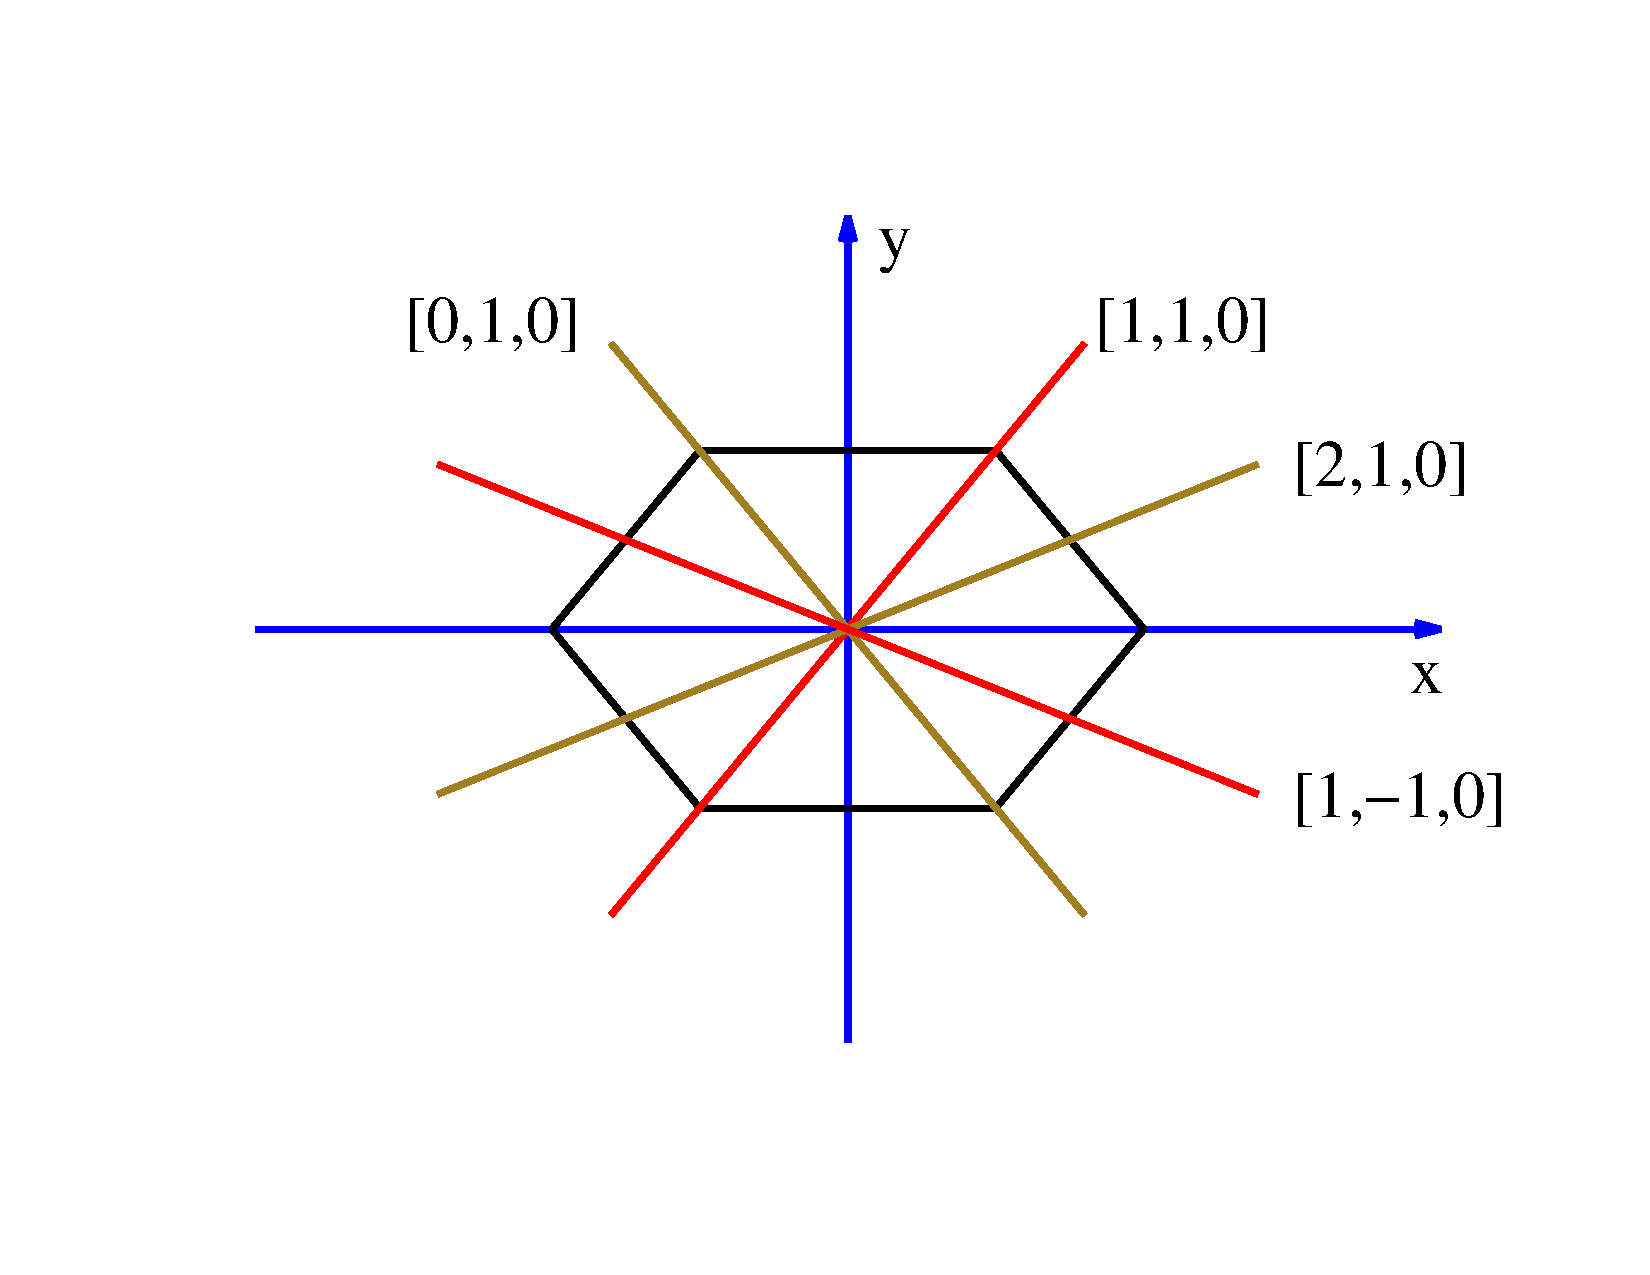
\includegraphics[width=15cm]{figure_hex.pdf} 
\end{center}
$[n_1,n_2,n_3]$ indicates a direction parallel
to the Bravais lattice $n_1 {\bf a}_1 + n_2 {\bf a}_2 + n_3 {\bf a}_3$
where ${\bf a}_1$ is along $x$, ${\bf a}_2$ is rotated 
of $120^\circ$ in the $xy$ plane and ${\bf a}_3$ is parallel to the $z$
axis.

\subsection{\color{web-blue}SU(2)}
The application of the rotation operator to a two-component spinor 
wavefunction requires the $2\times2$ matrices of the $SU(2)$ group.
The operation of $SU(2)$ in spin space can be defined by the Cayley-Klein
parameters ($a$ and $b$):
\begin{equation}
U=\left( \begin{array}{cc}
a, & b
\\
-b^*, & a^*
\end{array}
\right).
\nonumber
\end{equation}
There are two matrices of the double point group (differing by a global
sign) that correspond to the same rotation when the difference of $2\pi$ in
the rotation angle is neglected. In order to define the
matrices of the point group it is necessary to choose one $SU(2)$ matrix
for each rotation. The choice is not obvious for $180^\circ$ rotations.
Ref.[11] suggests the following choice of the Cayley-Klein parameters: 
\begin{verbatim}
     1   E       
             a=  1.00  0.00    b=  0.00  0.00   
     2   2z      
             a=  0.00 -1.00    b=  0.00  0.00    
     3   2y      
             a=  0.00  0.00    b= -1.00  0.00    
     4   2x      
             a=  0.00  0.00    b=  0.00 -1.00   
     5   2xy     
             a=  0.00  0.00    b= -0.71 -0.71    
     6   2x-y    
             a=  0.00  0.00    b=  0.71 -0.71     
     7   4-z     
             a=  0.71  0.71    b=  0.00  0.00  
     8   4z      
             a=  0.71 -0.71    b=  0.00  0.00   
     9   2xz     
             a=  0.00 -0.71    b=  0.00 -0.71  
    10   2x-z    
             a=  0.00 -0.71    b=  0.00  0.71     
    11   4y      
             a=  0.71  0.00    b= -0.71  0.00   
    12   4-y     
             a=  0.71  0.00    b=  0.71  0.00   
    13   2yz     
             a=  0.00 -0.71    b= -0.71  0.00  
    14   2y-z    
             a=  0.00 -0.71    b=  0.71  0.00  
    15   4-x     
             a=  0.71  0.00    b=  0.00  0.71  
    16   4x      
             a=  0.71  0.00    b=  0.00 -0.71   
    17   3-x-y-z 
             a=  0.50  0.50    b=  0.50  0.50    
    18   3-xyz   
             a=  0.50 -0.50    b= -0.50  0.50   
    19   3xy-z   
             a=  0.50  0.50    b= -0.50 -0.50   
    20   3x-yz   
             a=  0.50 -0.50    b=  0.50 -0.50  
    21   3xyz    
             a=  0.50 -0.50    b= -0.50 -0.50  
    22   3-xy-z  
             a=  0.50  0.50    b= -0.50  0.50    
    23   3x-y-z  
             a=  0.50  0.50    b=  0.50 -0.50    
    24   3-x-yz  
             a=  0.50 -0.50    b=  0.50  0.50    
    25   6z      
             a=  0.87 -0.50    b=  0.00  0.00    
    26   6-z     
             a=  0.87  0.50    b=  0.00  0.00    
    27   3z      
             a=  0.50 -0.87    b=  0.00  0.00    
    28   3-z     
             a=  0.50  0.87    b=  0.00  0.00    
    29   21-10   
             a=  0.00  0.00    b=  0.50 -0.87      
    30   2210    
             a=  0.00  0.00    b= -0.50 -0.87    
    31   2010    
             a=  0.00  0.00    b=  0.87 -0.50     
    32   2110    
             a=  0.00  0.00    b= -0.87 -0.50    
\end{verbatim}
for almost all groups except $D_3$, $C_{3v}$, and $D_{3d}$ for which
a different sign choice is necessary to keep in the same class the three
$C_2$ or $\sigma_v$ operations. \qe\ uses 
Ref.[11] conventions for all groups, without any sign change for
$D_3$, $C_{3v}$, and $D_{3d}$ operations. For these groups we use the
matrices written above changing the character table of the double point 
groups accordingly. 

\newpage
\section{\color{coral}Bibliography}
\begin{enumerate}

\item
P.W. Atkins, M.S. Child, and C.S.G. Phillips, ``Tables for group theory'',
Oxford University Press (1970). (Reference for character tables).

\item
G.F. Koster, J.O. Dimmok, R.G. Wheeler, and H. Statz, ``Properties
of the thirty-two point groups'', M.I.T Press, Cambridge (1963). 
(Reference for character tables of double groups).

\item
D.M. Bishop `Group theory and chemistry', Dover Publication, New York, (1973).
(An introduction to group theory).

\item
G. Burns and M. Glazer, `Space groups for solid state scientists', Academic Press
(2013). (Crystallographic symmetry concepts explained in detail). 

\item
M. Tinkham, `Group theory and quantum mechanics', Dover Publications, New York,
(1992). (More advanced treatment of group theory applied to atoms, molecules,
and solids).

\item
V. Heine, `Group theory in quantum mechanics', Pergamon Press, New York (1990).
(At the same level of the previous one, advanced treatment).

\item
M. Hamermesh, `Group theory and its application to physical problems',
Addison-Wesley, Massachussetts (1962). 
(Advanced and complete, contains more material than necessary to
understand the present notes).

\item
G.F. Koster, ``Space group and their representations'', Academic Press (1957).
(A concise explanation of the space group representations. Point
group representation tables as in Ref. 2).

\item
M. Lax, ``Symmetry principles in solid state and molecular physics'',
J. Wiley \& Sons, New York (1974).
(Advanced, more than the previous one for space group representations).

\item
O.V. Kovalev, ``Irreducible representations of the space groups'',
Academy of Science, USSR Press, Kiev (1961); in English
Gordon and Breach Science Publishers, New York (1965).
(A compilation of Tables of Irreducible representations of the space groups).

\item
S. K. Kim, `Group Theoretical methods and applications to molecules and 
crystal',
Cambridge University Press, Cambridge (1999). 
(A compact presentation of many concepts relevant to molecules and solids.
Advanced).

\item
M. I. Aroyo, A. Kirov, C. Capillas, J. M. Perez-Mato, and H. Wondratschek,
``Bilbao Crystallographic Server II: Representations of crystallographic 
point groups and space groups'', Acta Cryst. A62, 115-128 (2006).
(Detailed information on group-subgroups relationships).

\end{enumerate}

\end{document}
